\documentclass[12pt]{article}
\usepackage[utf8]{inputenc}
\usepackage[T1]{fontenc}
\usepackage{geometry}
\geometry{margin=1in}
\usepackage{setspace}
\linespread{1.1}
\setlength{\parindent}{0pt}
\setlength{\parskip}{0.5ex plus 0.2ex minus 0.1ex}
\usepackage{lmodern}
\usepackage{amsmath,amssymb}
\DeclareMathSizes{10.95}{10}{7}{5}
\DeclareMathSizes{10}{9}{6.5}{5}
\DeclareMathSizes{9}{8}{6}{5}
\DeclareMathSizes{8}{7}{5}{5}
\DeclareMathSizes{7}{6}{5}{5}
\usepackage{booktabs}
\usepackage{array}
\usepackage{graphicx}
\usepackage{float}
\usepackage{hyperref}
\usepackage{xcolor}
\usepackage{etoolbox}
\usepackage{caption}
\captionsetup{justification=centering,singlelinecheck=false}
\captionsetup[figure]{font=footnotesize,skip=4pt}
\captionsetup[table]{font=footnotesize,skip=4pt}
\AtBeginEnvironment{table}{\scriptsize}

\newenvironment{algorithm}[1][]{\begin{figure}[H]\small}{\end{figure}}
\newenvironment{algorithmic}[1][]{\begin{quote}\small}{\end{quote}}
\newcommand{\Require}{\par\noindent\textbf{Input:} }
\newcommand{\Ensure}{\par\noindent\textbf{Output:} }
\newcommand{\State}{\par\noindent}
\newcommand{\For}[1]{\par\noindent\textbf{for} #1 \textbf{do}}
\newcommand{\EndFor}{\par\noindent\textbf{end for}}
\newcommand{\If}[1]{\par\noindent\textbf{if} #1 \textbf{then}}
\newcommand{\EndIf}{\par\noindent\textbf{end if}}
\newcommand{\Comment}[1]{\hfill{\(\triangleright\) #1}}
\renewenvironment{abstract}{%
  \begin{center}
  \bfseries\abstractname
  \end{center}
  \small\noindent\ignorespaces
}{\par\normalsize}

\hypersetup{
  colorlinks=true,
  linkcolor=black,
  citecolor=black,
  urlcolor=blue
}

\title{\vspace{-1.8cm}\textbf{Reboosting the Power of Kernel Two-Sample Tests: Reveiew and Extensions based on MMMD Strategy}}
\author{\footnotesize Dechao Huang 23300660009\quad Ruijie Li 24300720157\quad Ziheng Zheng 23307110079\quad Yao Yu 23300660008}
\date{June 2026}

\begin{document}
\maketitle

\begingroup
\setstretch{0.98}
\setlength{\parskip}{0pt}
\setlength{\abovedisplayskip}{3pt}
\setlength{\belowdisplayskip}{3pt}
\setlength{\textfloatsep}{5pt}
\vspace{-1.0em}
\begin{abstract}
We review Mahalanobis aggregated maximum mean discrepancy (MMMD), a kernel two-sample test that combines correlated MMD statistics rather than selecting one bandwidth. The group reproduced the original testing framework and studied extensions involving covariance stabilization, alternative kernel constructions, and image representations. Across MNIST and biomedical image datasets, power depended on both the testing statistic and the feature space; the later sections therefore report power together with matched-null calibration and numerical diagnostics. Member contributions are Ruijie Li (Section~3, Appendix~A), Ziheng Zheng (Section~4, Appendix~B), Dechao Huang (Section~5, Appendix~C), and Yao Yu (Section~6, Appendix~D).
\end{abstract}
\small
\section{Background and motivation}
Given independent samples $X_1,\ldots,X_m\sim P$ and $Y_1,\ldots,Y_n\sim Q$, the two-sample problem tests $H_0:P=Q$ against $H_1:P\neq Q$. Biomedical alternatives need not be mean shifts: they may involve mixture proportions, covariance, rare subpopulations, morphology, or acquisition effects. Maximum mean discrepancy (MMD) compares the kernel mean embeddings of $P$ and $Q$ and is an omnibus test when a characteristic kernel is used \cite{gretton2012}. Its finite-sample power, however, can depend strongly on kernel bandwidth and, for images, on the representation supplied to the kernel. Kernel learning and aggregation address the first issue \cite{liu2020,schrab2023}; our experiments also examine the second by comparing raw measurements with learned features.

\section{MMMD in the reviewed paper}
For kernels $k_1,\ldots,k_R$, let $\widehat{\boldsymbol m}=(\widehat{\mathrm{MMD}}^2_{k_1},\ldots,\widehat{\mathrm{MMD}}^2_{k_R})^\top$ and let $\widehat\Sigma$ estimate their joint covariance. MMMD uses the Mahalanobis statistic
\[
T_{\mathrm{MMMD}}=\widehat{\boldsymbol m}^{\top}(\widehat\Sigma+\lambda I)^{-1}\widehat{\boldsymbol m},
\]
with a multiplier bootstrap to estimate the null cutoff \cite{chatterjee2025}. The covariance weighting discounts redundant kernel components and combines discrepancies that are informative at different scales. The same mechanism also creates the principal practical limitation: with many highly correlated components and small samples, $\widehat\Sigma$ may be ill-conditioned and calibration may become unstable. The subsequent experiments retain this testing framework while studying covariance stabilization and alternative data representations.
\normalsize
\endgroup
\clearpage

\section{NEW-MMMD: stabilizing and accelerating the covariance}
\label{sec:newmmmd}

This section presents our own methodological extension to the reviewed paper, rather than part of the original MMMD method. NEW-MMMD first prunes the candidate kernel grid by lazy pivoted Cholesky. At each step, the algorithm selects the kernel with the largest unexplained residual and stops when the largest relative residual falls below $\varepsilon$. The selected set $S$ has $q<R$ numerically independent kernels, and both the statistic and bootstrap cut-off are recomputed on $\widehat{\Sigma}_{S,S}$. Thus pruning becomes part of the calibrated test rather than a post-hoc diagnostic; Appendix~\ref{app:newmmmd-algorithm} gives the full pseudocode.

NEW-MMMD also exploits Gaussian and Laplace multiplicative closure. After reparameterization, both families can be written as $K_t(x,y)=\exp\{-t d(x,y)\}$, with $t=1/\sigma^2$ for Gaussian kernels and $t=1/\sigma$ for Laplace kernels. The covariance and product identities are
\[
  \widehat{\Sigma}_{ab}\propto \langle C K_{t_a} C, C K_{t_b} C\rangle_F,
  \qquad K_{t_a}\circ K_{t_b}=K_{t_a+t_b}.
\]
Thus an arithmetic $t$-grid needs only $2R-1$ cached product kernels instead of $R^2$ repeated sample scans. After Cholesky selection, the multiplier bootstrap uses only the $q$ retained kernels. Table~\ref{tab:newmmmd-main-complexity} summarizes the resulting change in computational order; the derivation and implementation details are in Appendix~\ref{app:newmmmd-complexity}.

\begin{table}[H]
\centering
\caption{Main computational effect of NEW-MMMD. Here $R$ is the candidate kernel count, $q$ is the number selected by pivoted Cholesky, $m$ is the sample size, and $B$ is the number of bootstrap draws.}
\label{tab:newmmmd-main-complexity}
\scriptsize
\begin{tabular}{lcc}
\toprule
Stage & Paper/naive MMMD & NEW-MMMD \\
\midrule
Covariance build & $O(R^2m^3)$ & $O(Rm^2)$ \\
Kernel selection & --- & $O(Rq^2)$ \\
Bootstrap & $O(BRm^2)$ & $O(Bqm^2)$ \\
Matrix inverted & $R\times R$ & $q\times q$, usually $q<R$ \\
\bottomrule
\end{tabular}
\end{table}

Table~\ref{tab:newmmmd-main-evidence} collects the headline checks. The fast covariance matches the naive estimator to about $8.3\times10^{-16}$, but at matched $R=13$ it builds the covariance about $16\times$ faster and is $4.8\times$ faster end to end. On the raw-pixel PathMNIST null, GEXP-5 rejects at about twice the nominal level, while NEW-MMMD stays near $0.05$ after pruning to a well-conditioned $4\times4$ or $5\times5$ block; size-corrected power is then essentially tied.

\begin{table}[H]
\centering
\caption{Representative empirical evidence for NEW-MMMD. Timing uses the synthetic $n=700$ experiment; calibration and conditioning use the raw-pixel PathMNIST matched null at $n=120$.}
\label{tab:newmmmd-main-evidence}
\scriptsize
\setlength{\tabcolsep}{5pt}
\begin{tabular}{lcc}
\toprule
Quantity & Paper/naive benchmark & NEW-MMMD \\
\midrule
Covariance-build time & 16.37 s (GEXP-rich-13) & 1.04 s (NEW-13) \\
End-to-end time & 28.49 s (GEXP-rich-13) & 5.90 s (NEW-13) \\
Matched-null Type-I & 0.106 (GEXP-5) & 0.040 \\
Condition number inverted & $2.47\times10^5$ (GEXP-5) & $4.19\times10^4$ \\
Size-corrected power & 0.304 (GEXP-5) & 0.286 \\
\bottomrule
\end{tabular}
\end{table}

In short, NEW-MMMD makes the covariance layer faster and more stable while keeping the same MMMD testing principle. Its power gains depend on the kernel grid, but its scalability and Type-I calibration are the main advantages over the original implementation.

\section{Numerical extensions to the MMMD framework}

\subsection{Experimental setup}

The original paper evaluates MMMD mainly under Gaussian mean- and variance-shift alternatives. We extend the numerical study to heavy-tailed contamination, small covariance changes, non-Euclidean sample geometry, and partial-population mixtures. Unless stated otherwise, experiments use synthetic data with $d=30$, AR(1) covariance ($\rho=0.5$), $n=100$, multiplier bootstrap with $B=500$, and $N=150$--$200$ Monte Carlo trials. We compare GEXP, LAP, and MIXED kernel families; detailed grids are in Appendix~\ref{app:numext}.

For contamination, we set $P=\mathcal{N}(0,\Sigma)$ and $Q=(1-\varepsilon)\mathcal{N}(0,\Sigma)+\varepsilon t_{10}(0,\Sigma)$. With GEXP and $r=5$, the minimum contamination fraction reaching power 0.80 is $\varepsilon_{\min}=0.625$.

For variance scaling, $P=\mathcal{N}(0,\Sigma_0)$ and $Q=\mathcal{N}(0,k\Sigma_0)$. All three MMMD variants reach power $\geq0.80$ at $k_{\min}=1.25$, whereas single-kernel Gaussian MMD requires $k_{\min}=1.40$ (Figure~\ref{fig:var-sensitivity}, Table~\ref{tab:var-sensitivity}).

\subsection{Type-I error calibration and ROC analysis}

Type-I error is near the nominal 0.05 level for all families at $r=3$ and $r=5$. At $r=10$, GEXP inflates to 0.120, MIXED rises to 0.070, and LAP remains at 0.050, suggesting that GEXP should be kept to $r\leq5$ while LAP is more tolerant of larger kernel banks. ROC analysis at $k=1.25$ gives false-positive rates near 0.05 and true-positive rates of 0.435--0.500, with only small power differences across families (Figure~\ref{fig:roc}, Table~\ref{tab:type1}).

\subsection{Graph-MMMD: construction, calibration, and skewness robustness}

We also form a $k$-nearest-neighbor graph on the pooled sample $\mathcal{X}_m\cup\mathcal{Y}_n$, build the graph Laplacian $L$, and use heat kernels $K_t=\exp(-tL)$ over a diffusion-time grid. Under Gaussian AR(1), scaled Gaussian, skew-normal, and multivariate Laplace nulls, empirical Type-I errors are 0.027, 0.020, 0.020, and 0.033. A skewness sweep over standardized skewness 0.00--0.90 gives Type-I errors of 0.020--0.053 with no monotone drift, indicating that Graph-MMMD remains conservative under asymmetric nulls (Figures~\ref{fig:graph-type1}--\ref{fig:skew-type1}).

\subsection{Mixture reproduction and summary}

We reproduce the original normal-$t$ mixture experiment with $P=(1-p)\mathcal{N}(0,\Sigma_0)+pt_{10}(0,\Sigma_0)$ and $Q=(1-p)\mathcal{N}(0,1.25\Sigma_0)+pt_{10}(0,1.25\Sigma_0)$. Mixed MMMD achieves power 0.96, 0.80, and 0.58 at $p=0,0.4,1.0$, respectively, compared with 0.46, 0.31, and 0.35 for single-kernel MMD. Thus MMMD keeps a 2--5 fold power advantage across mixture proportions (Figure~\ref{fig:mixture}, Table~\ref{tab:mixture}).

Overall, multi-kernel MMMD outperforms single-kernel MMD for contamination, variance scaling, mixture, and graph-based alternatives. The main guidelines are to limit GEXP to $r\leq5$ or use LAP for larger banks, expect the largest relative gains under subtle distributional differences, and use graph kernels when non-Euclidean geometry is important without sacrificing calibration.

\section{CNN representation-assisted MMMD for image two-sample testing}
\label{sec:cnn-mmmd}

\begingroup
\setlength{\textfloatsep}{7pt plus 2pt minus 2pt}
\setlength{\intextsep}{6pt plus 2pt minus 2pt}
\setlength{\abovedisplayskip}{5pt}
\setlength{\belowdisplayskip}{5pt}
\captionsetup{font=small,skip=3pt}

Kernel two-sample tests depend on both the kernel and the representation supplied to it. We therefore compared raw pixels with features from a small CNN trained once on an independent labelled split and then frozen. Tests used cached features only. The first representation was the 128-dimensional penultimate layer (FC-128). The second aggregated a shallow layer, an intermediate layer, and FC-128, using either one Gaussian kernel per layer (three MMD components) or five bandwidths per layer (15 components). MMMD combined the resulting layer--kernel discrepancies through its usual Mahalanobis statistic.

MNIST additive-noise experiments provided an implementation check; PathMNIST then tested the same construction on colorectal histology images. In the class-mixture alternative, \texttt{mix635} and \texttt{mix835} shared labels 3 and 5 and differed by replacing label 6 with label 8. Formal PathMNIST runs used 10 outer repetitions, 500 independent tests per repetition, and 500 multiplier-bootstrap draws. Full power and null curves are reported in Appendix~\ref{app:dechao-cnn-mmmd}.

\begin{figure}[H]
\centering
\begin{minipage}[t]{0.48\textwidth}
\centering
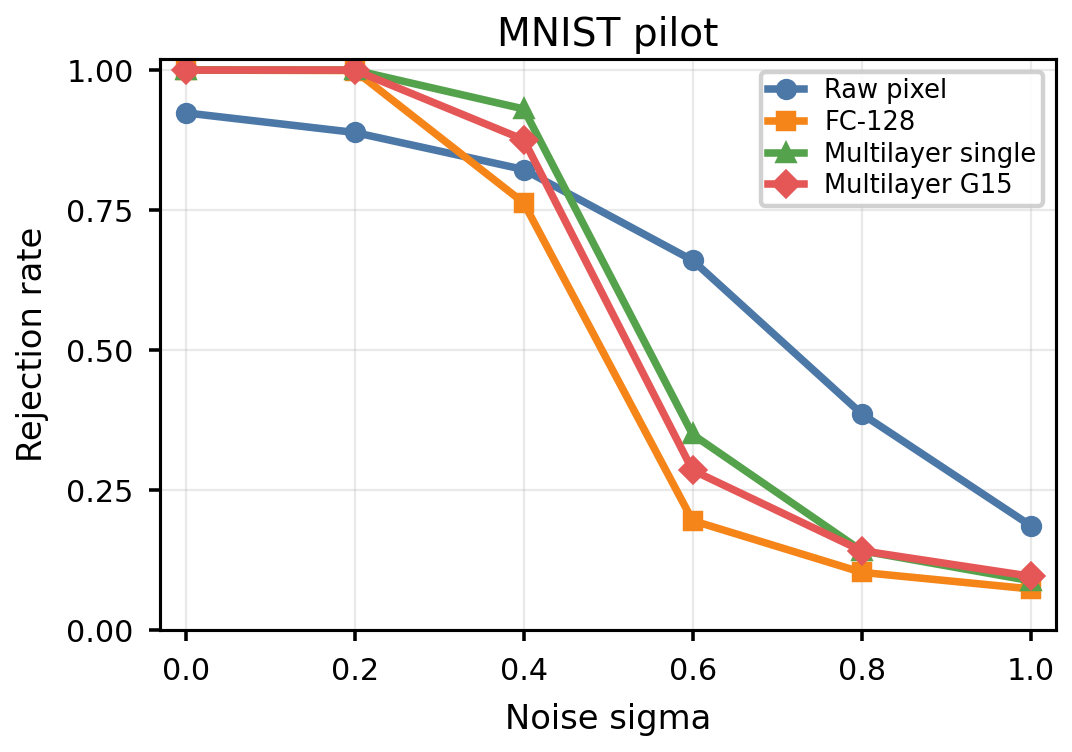
\includegraphics[width=\linewidth]{figures/dechao_mnist_pilot_power_simple.png}
\end{minipage}\hfill
\begin{minipage}[t]{0.48\textwidth}
\centering
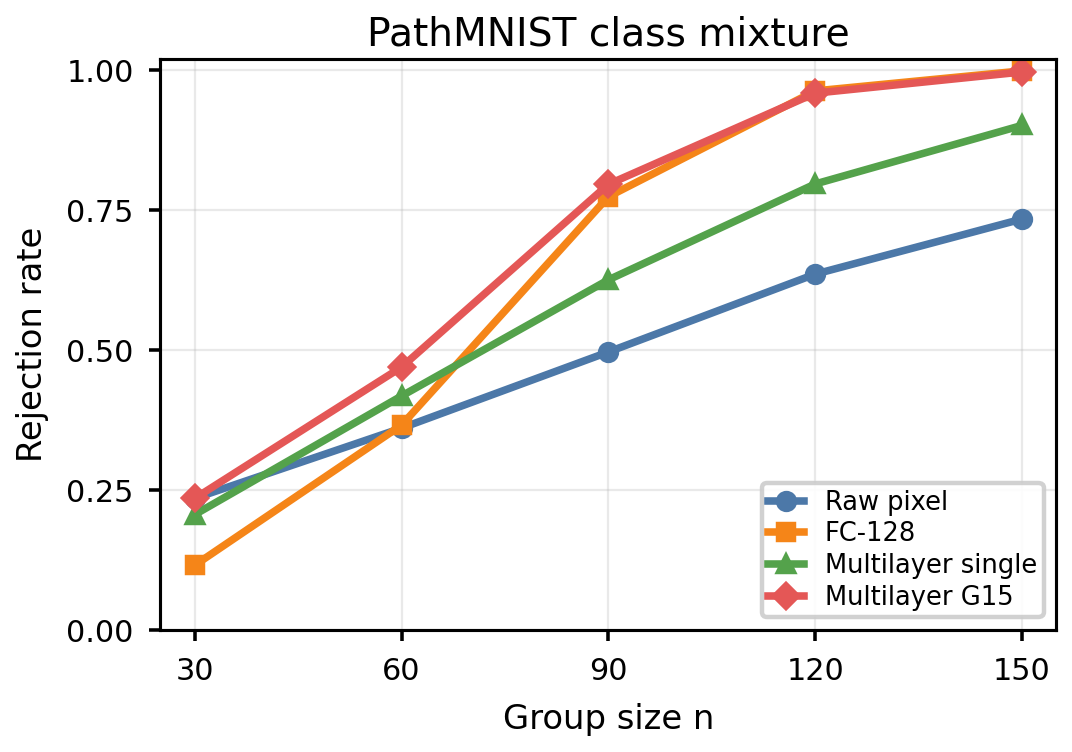
\includegraphics[width=\linewidth]{figures/dechao_pathmnist_class_power_simple.png}
\end{minipage}
\caption{Power comparisons on the MNIST pilot (left) and PathMNIST class-mixture alternative (right).}
\label{fig:dechao-main-pilot-class-power}
\end{figure}

\begin{table}[H]
\centering
\caption{Selected PathMNIST rejection rates. The matched null compares \texttt{mix635} with itself; center-shift alternatives compare source-holdout and external images within one label.}
\label{tab:dechao-main-rejection}
\scriptsize
\setlength{\tabcolsep}{3.6pt}
\begin{tabular}{llrrrr}
\toprule
Task & Setting & Raw & FC-128 & Multi-3 & Multi-15 \\
\midrule
Class mixture, $n=120$ & H1 & 0.636 & 0.963 & 0.797 & 0.959 \\
Class mixture, $n=120$ & H0 & 0.033 & 0.010 & 0.014 & 0.017 \\
Label 6 center shift, $n=50$ & H1 & 0.782 & 0.763 & 0.991 & 0.989 \\
Label 8 center shift, $n=50$ & H1 & 0.960 & 0.957 & 0.985 & 0.975 \\
\bottomrule
\end{tabular}
\end{table}

For the class-mixture alternative, FC-128 and the 15-component multilayer test were substantially more powerful than raw pixels, while the matched-null rates were below 0.05. The same-label source-vs-external experiment fixed the tissue class and therefore targeted center-associated variation rather than class composition. Multilayer features were especially sensitive for label 6, whereas raw pixels and FC-128 were already highly sensitive for label 8. Small-$n$ internal-null checks for the 15-component test were mildly liberal; the complete source-internal and external-internal checks appear in Appendix~\ref{app:dechao-cnn-mmmd}.

To locate the signal within FC-128, let $h(x)\in\mathbb{R}^{128}$ and let the frozen classifier logits be $Wh(x)+b$. Since softmax is invariant to a common logit shift, we used centered weights $W_c=(I_C-C^{-1}\mathbf 1\mathbf 1^\top)W$ and defined
\[
h_{\mathrm{sem}}=P_{\operatorname{row}(W_c)}h,
\qquad
h_{\mathrm{res}}=h-h_{\mathrm{sem}}.
\]
The first component affects class-relative logits; the second satisfies $W_ch_{\mathrm{res}}=0$ and is ignored by the final linear head. At representative sample sizes, the class mixture gave rejection rates 0.980, 0.958, and 0.955 for logits, semantic, and residual features, respectively. Label 6 center shift gave 0.858, 0.825, and 0.750, whereas label 8 gave 0.820, 0.840, and 0.958. Thus the label-8 difference was strongest in residual coordinates.

We checked whether this residual result was a dimensional artifact. The centered semantic subspace had rank at most eight; at $n=50$, the leading eight residual PCs, a random 8D residual projection, and the full residual representation gave rejection rates 0.965, 0.890, and 0.975. A label-8 PCA sweep reached 0.925 with two PCs and 0.960 with four PCs. We then assessed color/stain association using 15 RGB summaries (channel means, standard deviations, and 10th, 50th, and 90th percentiles). On held-out images these summaries explained 72.8\% of the top-eight residual source--external score, and score residualization reduced its AUC from 0.778 to 0.622. Color-only MMMD reached power 0.960 at $n=50$; after color-propensity matching, residual MMMD fell to 0.455, compared with a maximum matched-null rate of 0.110. Corresponding plots and matching diagnostics are provided in Appendix~\ref{app:dechao-cnn-mmmd}.

Overall, CNN features improved power for the PathMNIST class-mixture alternative, while the same-label label-8 comparison revealed a low-dimensional residual shift that was strongly associated with color/staining rather than uniquely with morphology.

\endgroup

\section{Beyond task-trained CNNs: frozen visual encoders and stabilized testing}

This section studies whether the feature space used before testing changes the behavior of MMMD-style two-sample tests. Most comparisons keep the testing layer fixed, so differences in power mainly reflect differences in representation rather than changes in the statistic itself.

\subsection{From CNN features to foundation encoders}

The starting point is the CNN-MMMD pipeline: train a small CNN, extract feature vectors, and run MMMD on the resulting feature matrices. This works well when labels are available, but it also makes the test depend on a dataset-specific training step. We therefore ask whether frozen foundation encoders can provide a useful representation layer without retraining. Raw pixels serve as the direct image-space baseline, task-trained CNN features serve as the supervised baseline, and CLIP and DINOv2 represent two frozen encoder families.

\subsection{Experimental protocol}

We report empirical power under mixture alternatives and empirical Type-I error under matched null settings. The experiments use three biomedical image benchmarks and four focused comparisons, summarized in Table~\ref{tab:foundation-exp-summary}. Dataset descriptions, mixture definitions, implementation paths, and the BloodMNIST/PathMNIST figure are given in Appendix~\ref{app:repr}.

\begin{table}[H]
\centering
\caption{Summary of the four representation experiments.}
\label{tab:foundation-exp-summary}
\scriptsize
\setlength{\tabcolsep}{3pt}
\begin{tabular}{>{\raggedright\arraybackslash}p{0.18\textwidth}
                >{\raggedright\arraybackslash}p{0.15\textwidth}
                >{\raggedright\arraybackslash}p{0.30\textwidth}
                >{\raggedright\arraybackslash}p{0.30\textwidth}}
\toprule
Experiment & Dataset & Comparison & Main readout \\
\midrule
Noise robustness & BloodMNIST-224 & Raw pixels, CLIP, DINOv2, CNN under additive noise & CNN remains strongest at heavy noise; frozen encoders degrade faster. \\
Small-patch alignment & PathMNIST-28 & Frozen encoders versus task-trained CNN baselines & DINOv2 catches up at larger \(n\), while small samples still favor CNN features. \\
Sample-size scaling & NCT-CRC & Raw pixels, CLIP, CNN, and DINOv2 across \(n\) & DINOv2 becomes strongest at large \(n\); raw pixels remain sample inefficient. \\
Testing-layer stabilization & NCT-CRC & GEXP-5 versus NEW-MMMD with fixed representations & NEW-MMMD improves calibration and conditioning more consistently than power. \\
\bottomrule
\end{tabular}
\end{table}

\begin{figure}[H]
\centering
\begin{minipage}[t]{0.49\textwidth}
\centering
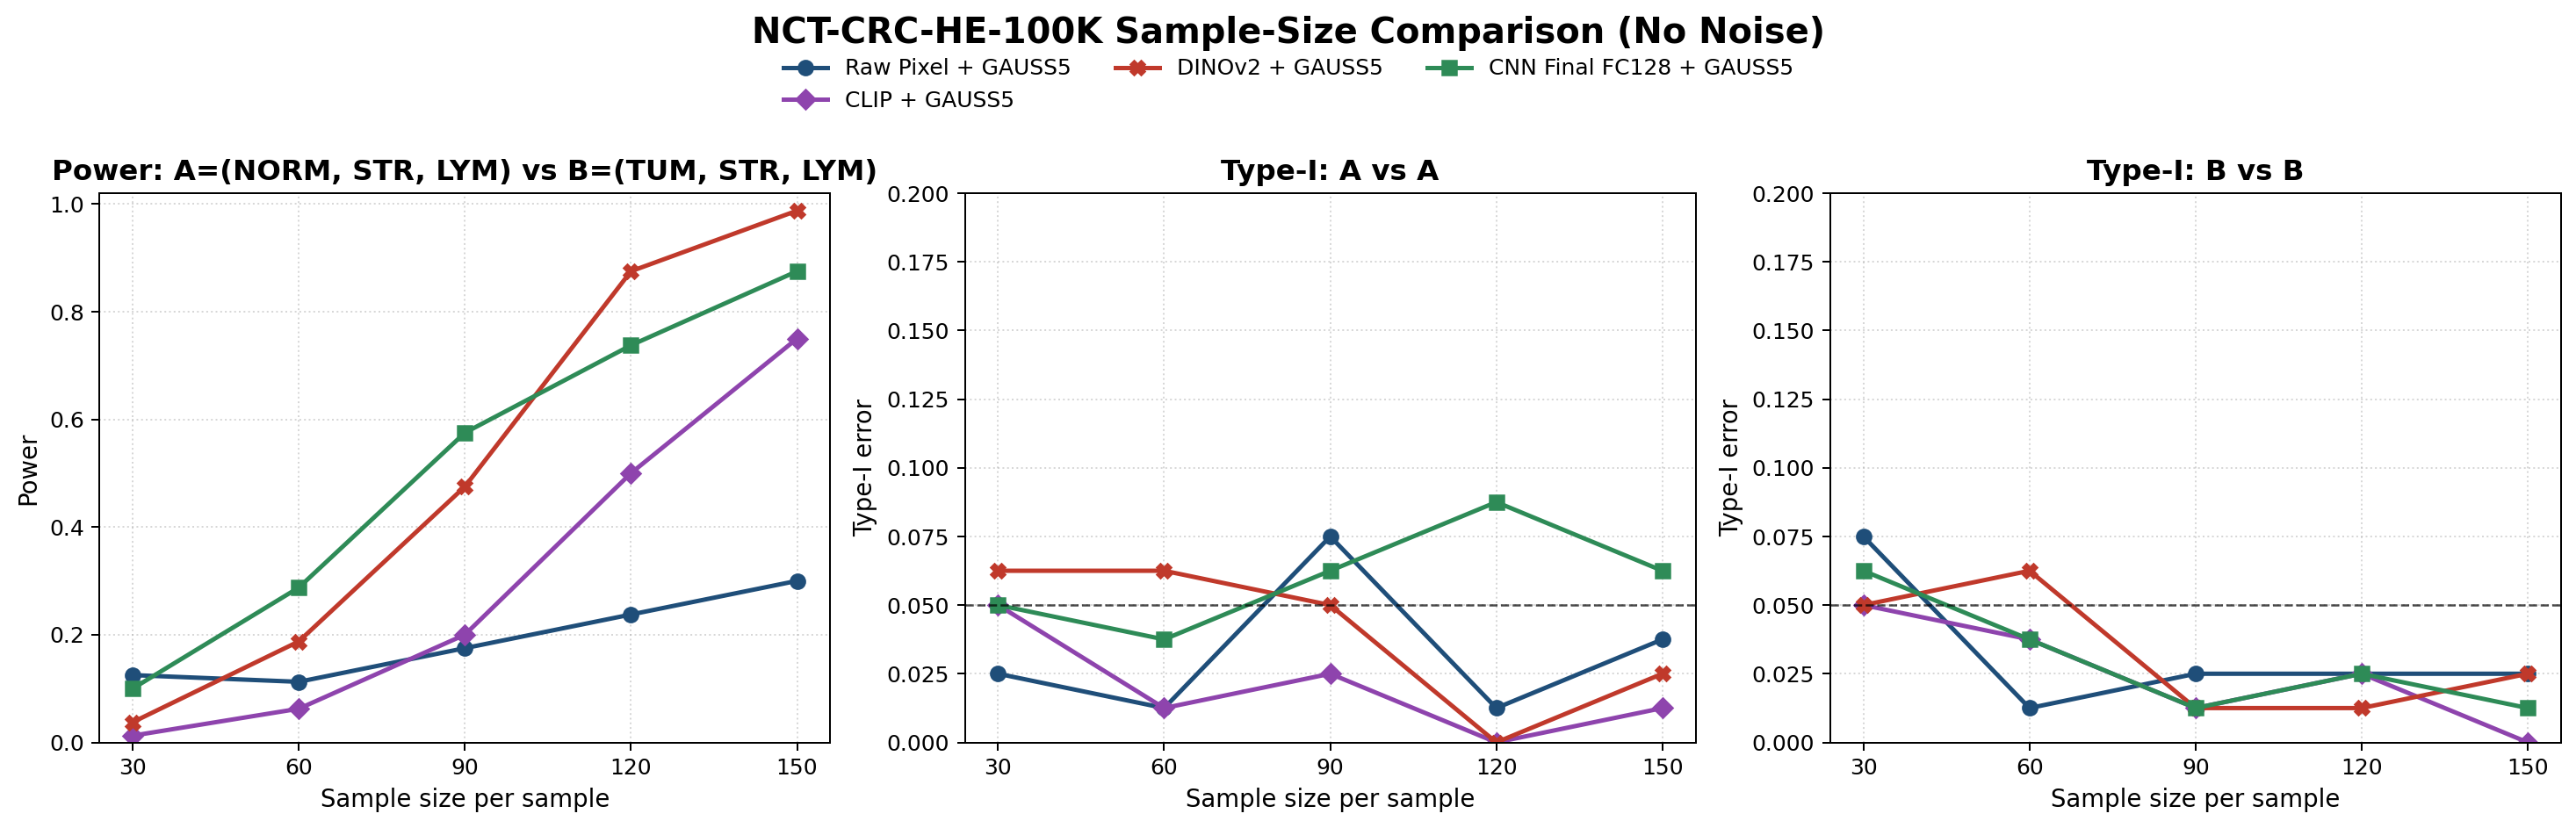
\includegraphics[width=\linewidth]{figures/nctcrc_sample_size_comparison.png}
\end{minipage}\hfill
\begin{minipage}[t]{0.49\textwidth}
\centering
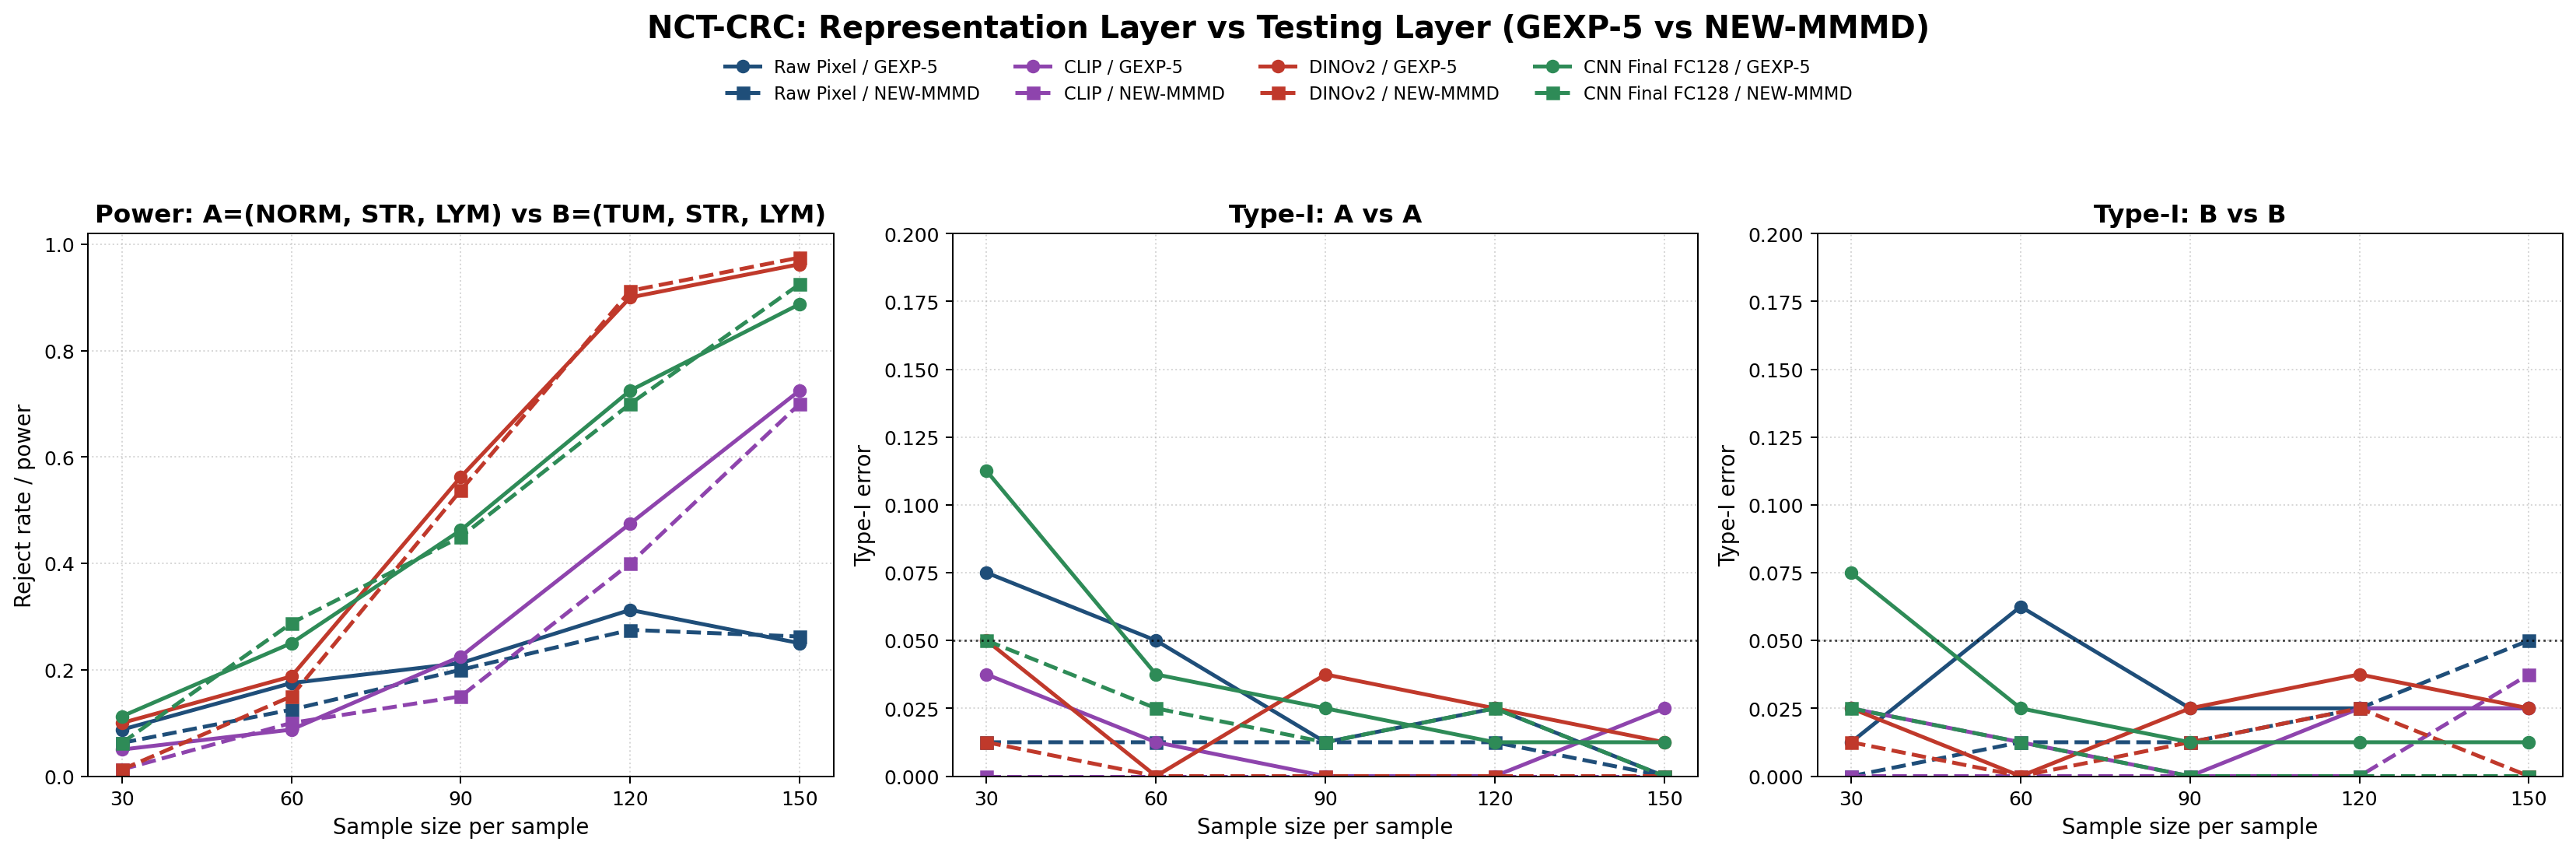
\includegraphics[width=\linewidth]{figures/nctcrc_lrj_all_representations.png}
\end{minipage}
\caption{NCT-CRC representation and testing-layer experiments.}
\label{fig:nct-newmmmd-main}
\end{figure}

\subsection{Insights and limitations}

\textbf{Noise robustness.} BloodMNIST shows that supervised CNN features can be more robust than frozen foundation embeddings under strong additive noise, so generic pretraining is not automatically best.

\textbf{Small-patch pathology.} PathMNIST shows that DINOv2 can approach task-trained CNN baselines as sample size increases, but very small pathology patches still benefit from dataset-specific supervision.

\textbf{Sample-size scaling.} NCT-CRC shows that representation rankings change with sample size: DINOv2 is strongest at large \(n\), while raw pixels are consistently inefficient.

\textbf{Testing-layer stabilization.} The NEW-MMMD comparison shows that improving the testing layer mainly helps calibration and covariance conditioning; power gains still depend on the representation and sample size.

\textbf{Limitations.} These experiments are limited by computational resources and time, so they focus on representative feature spaces rather than an exhaustive benchmark. Future work could test more foundation models, more medical datasets, richer class combinations, noise and domain-shift settings, and fine-tuned or domain-adapted encoders.

\clearpage
\appendix
\section{NEW-MMMD: detailed numerical experiments}
\label{app:newmmmd}

This appendix details the experiments behind Section~\ref{sec:newmmmd}. Three settings are used: a reproduction of the paper's Figure~1(b) on synthetic Gaussian scale shifts that checks power parity, a time-complexity study that isolates the covariance speed-up, and a high-dimensional PathMNIST two-sample test that exposes the ill-conditioning the method targets.

\subsection{Algorithm and cost details}
\label{app:newmmmd-algorithm}
\label{app:newmmmd-complexity}

This subsection gives the details suppressed from the main text. Write $\widetilde{K}_a=C_m\widehat{K}_aC_m$ for the centered Gram matrix of kernel $a$ on the $X$ sample. Up to the constant factor in the paper's covariance estimator,
\[
  \widehat{\Sigma}_{ab}\propto \langle \widetilde{K}_a,\widetilde{K}_b\rangle_F.
\]
Thus $\widehat{\Sigma}$ is a Gram matrix whose ``observations'' are themselves vectorized centered Gram matrices. If two bandwidths produce nearly identical similarity matrices, then $\operatorname{vec}(\widetilde{K}_a)$ and $\operatorname{vec}(\widetilde{K}_b)$ are nearly collinear, and the covariance matrix becomes ill-conditioned. NEW-MMMD removes these redundant directions before inversion.

For a generic kernel family, define a covariance-column oracle
\[
  \mathcal{C}(p)=\widehat{\Sigma}_{\cdot,p}\in\mathbb{R}^{R}.
\]
The lazy pivoted-Cholesky selection uses this oracle rather than forming the whole $R\times R$ covariance matrix in advance. Its inputs are the candidate kernels $K_1,\ldots,K_R$, the diagonal entries $\widehat{\Sigma}_{jj}$, a relative tolerance $\varepsilon$, and optionally a maximum selected size $q_{\max}$. It returns a selected index set $S=\{p_1,\ldots,p_q\}$, a low-rank factor $L\in\mathbb{R}^{R\times q}$ describing the explained covariance geometry, and the selected covariance block $\widehat{\Sigma}_{S,S}$ used by the final MMMD statistic.

Algorithm~\ref{alg:lazy-pchol} gives the selection step in pseudocode.

\begin{algorithm}[H]
\caption{Lazy pivoted-Cholesky kernel selection}
\label{alg:lazy-pchol}
\begin{algorithmic}[1]
\Require Candidate kernels $K_1,\ldots,K_R$; diagonal entries $\widehat{\Sigma}_{jj}$; covariance-column oracle $\mathcal{C}(p)=\widehat{\Sigma}_{\cdot,p}$; tolerance $\varepsilon$; optional cap $q_{\max}$.
\Ensure Selected kernel set $S$ and selected covariance block $\widehat{\Sigma}_{S,S}$.
\State $S\gets\varnothing$, $L\gets$ empty matrix, $d_{\max}\gets\max_j\widehat{\Sigma}_{jj}$
\For{$j=1,\ldots,R$}
  \State $r_j\gets\widehat{\Sigma}_{jj}$
\EndFor
\For{$t=1,\ldots,q_{\max}$}
  \State $p\gets\arg\max_{j\notin S} r_j$
  \If{$r_p\le\varepsilon d_{\max}$}
    \State \textbf{break}
  \EndIf
  \State $c\gets\mathcal{C}(p)$ \Comment{compute only the pivot column when needed}
  \State append $p$ to $S$
  \For{$j=1,\ldots,R$}
    \State $L_{j,t}\gets\big(c_j-\sum_{s<t}L_{j,s}L_{p,s}\big)/\sqrt{r_p}$
  \EndFor
  \For{$j=1,\ldots,R$}
    \State $r_j\gets r_j-L_{j,t}^2$
  \EndFor
\EndFor
\State Form or recompute $\widehat{\Sigma}_{S,S}$ from the selected columns.
\State Recompute the MMMD statistic and multiplier-bootstrap cut-off using only kernels in $S$.
\end{algorithmic}
\end{algorithm}
The residual $r_j^{(t)}$ is the Schur-complement variance left after projecting kernel $j$ onto the span of the selected kernels. A small residual means that the corresponding centered Gram matrix contributes almost no new covariance direction, so removing it improves conditioning without discarding an independent scale. Selection is not followed by using the old critical value: both $T_{m,n}$ and the multiplier-bootstrap cut-off are recomputed on the selected kernel bank.

For Gaussian and Laplace kernels the column oracle can be made much faster. Use the common parameterization
\[
  K_t(x,y)=\exp(-t d(x,y)),
\]
where $d(x,y)=\lVert x-y\rVert_2^2$ and $t=1/\sigma^2$ for Gaussian kernels, while $d(x,y)=\lVert x-y\rVert_2$ and $t=1/\sigma$ for Laplace kernels. Then
\[
  K_{t_a}(x,y)K_{t_b}(x,y)=K_{t_a+t_b}(x,y).
\]
This closure is useful because the centered Frobenius product can be expanded as
\[
  \langle C_mK_aC_m,C_mK_bC_m\rangle_F
  =H(t_a+t_b)-\frac{2}{m}s_a^{\top}s_b+\frac{1}{m^2}S_aS_b,
\]
where
\[
  H(u)=\sum_{i,j=1}^{m}\exp(-uD_{ij}),\qquad
  s_a=K_a\mathbf{1},\qquad
  S_a=\mathbf{1}^{\top}K_a\mathbf{1}.
\]
Here $D_{ij}=d(X_i,X_j)$. On an arithmetic $t$-grid, $t_a+t_b$ has only $2R-1$ distinct values, so all needed $H(u)$ values can be cached with $O(Rm^2)$ sample-pair scans instead of recomputing a separate scan for each of the $R^2$ covariance pairs. The row-sum terms $s_a$ and $S_a$ are also cached; a lazy query for column $p$ then combines the stored $H(t_j+t_p)$ values with $s_j^{\top}s_p$ and $S_jS_p$ for all $j$. Algorithm~\ref{alg:closure-cov} records the full covariance construction; in the lazy version, the last loop is evaluated only for queried pivot columns.

\begin{algorithm}[H]
\caption{Closure-based covariance construction for Gaussian/Laplace kernels}
\label{alg:closure-cov}
\begin{algorithmic}[1]
\Require Sample $X_1,\ldots,X_m$; parameters $t_1,\ldots,t_R$; distance $d(\cdot,\cdot)$; sample ratio $\widehat{\rho}$.
\Ensure Covariance matrix $\widehat{\Sigma}$, or a column oracle $\mathcal{C}(p)$ for Algorithm~\ref{alg:lazy-pchol}.
\State Compute $D_{ij}\gets d(X_i,X_j)$ for all $1\le i,j\le m$.
\For{$a=1,\ldots,R$}
  \State $K_a\gets[\exp(-t_aD_{ij})]_{i,j=1}^m$
  \State $s_a\gets K_a\mathbf{1}$ and $S_a\gets\mathbf{1}^{\top}K_a\mathbf{1}$
\EndFor
\State $\mathcal{U}\gets\{t_a+t_b:1\le a\le b\le R\}$
\For{$u\in\mathcal{U}$}
  \State $H(u)\gets\sum_{i,j=1}^{m}\exp(-uD_{ij})$
\EndFor
\For{$a=1,\ldots,R$ and $b=1,\ldots,R$}
  \State $I_{ab}\gets H(t_a+t_b)-2s_a^{\top}s_b/m+S_aS_b/m^2$
  \State $\widehat{\Sigma}_{ab}\gets 2I_{ab}/\{\widehat{\rho}^{2}(1-\widehat{\rho})^{2}m^2\}$
\EndFor
\State Symmetrize $\widehat{\Sigma}\gets(\widehat{\Sigma}+\widehat{\Sigma}^{\top})/2$.
\end{algorithmic}
\end{algorithm}

The resulting cost is summarized in Table~\ref{tab:app-newmmmd-complexity}. The generic lazy Cholesky part costs $O(Rq^2)$ in algebra after the covariance columns are available. With closure-based caching, the dominant covariance construction is $O(Rm^2)$ on an arithmetic grid, and the bootstrap stage uses only $q$ kernels. Keeping lower-order terms, the combined Gaussian/Laplace route is approximately
\[
  O(dm^2+Rm^2+qmR+Rq^2+Bqm^2+B\log B),
\]
where $d$ is the data dimension and $B$ is the number of bootstrap draws. The simplified message is that the expensive sample-pair work scales with $R$ during covariance construction and with $q$ during bootstrap, rather than with all $R^2$ covariance pairs and all $R$ kernels.

\begin{table}[H]
\centering
\caption{Per-iteration cost of building the covariance and running the bootstrap, for $R$ candidate kernels, $q$ selected kernels, $m$ samples, and $B$ bootstrap draws.}
\label{tab:app-newmmmd-complexity}
\scriptsize
\begin{tabular}{lcc}
\toprule
Stage & Paper (naive) & NEW-MMMD \\
\midrule
Covariance build & $O(R^2 m^3)$ & $O(R m^2)$ \\
Kernel selection  & ---          & $O(R q^2)$ \\
Bootstrap         & $O(B R m^2)$ & $O(B q m^2)$ \\
\bottomrule
\end{tabular}
\end{table}
\begin{figure}[H]
\centering
\begin{minipage}[t]{0.49\textwidth}
  \centering
  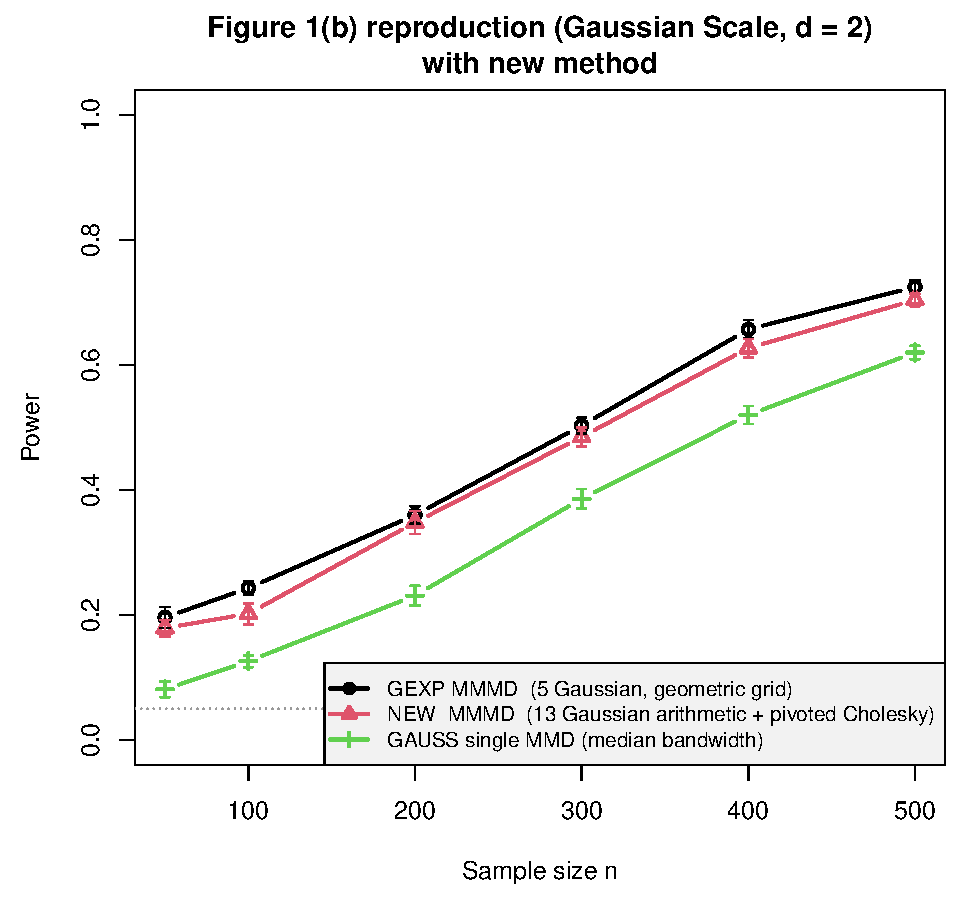
\includegraphics[width=\linewidth,height=0.30\textheight,keepaspectratio]{figures/Figure1b_with_NewMethod.pdf}
\end{minipage}\hfill
\begin{minipage}[t]{0.49\textwidth}
  \centering
  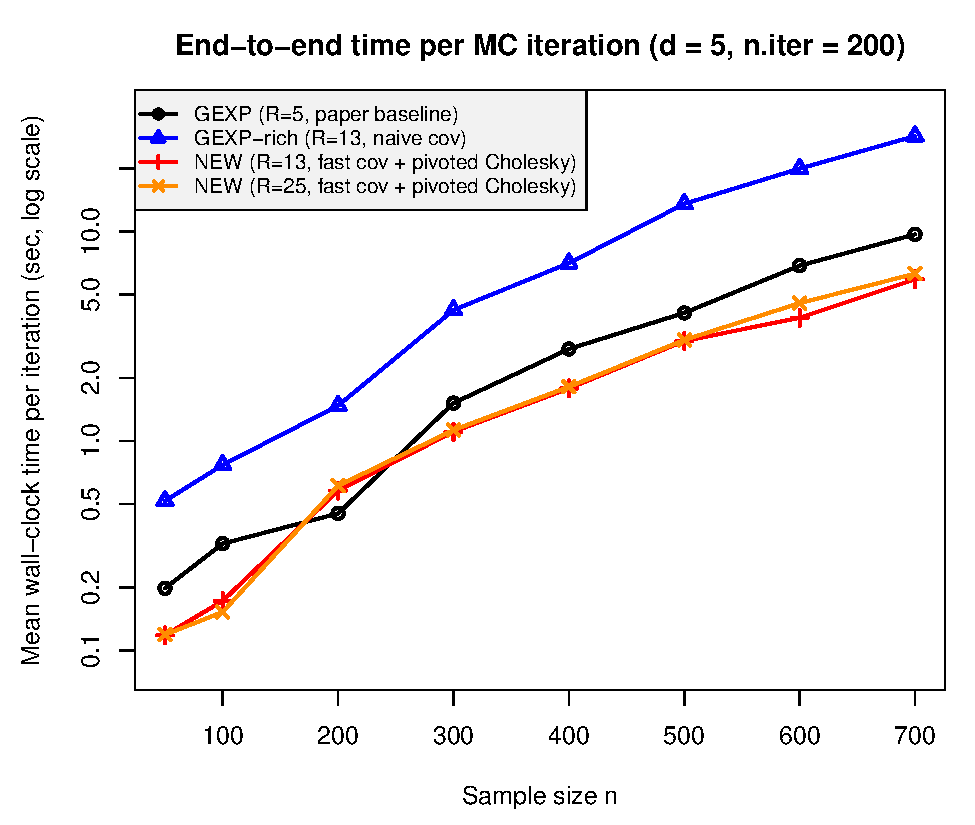
\includegraphics[width=\linewidth,height=0.30\textheight,keepaspectratio]{figures/TimeComparison_total.pdf}
\end{minipage}
\caption{NEW-MMMD on synthetic Gaussian scale shifts. Left: power versus sample size ($d=2$), matching the paper's multi-kernel test and beating single-kernel MMD. Right: time per iteration versus sample size ($d=5$), showing the covariance and end-to-end speed-ups at matched kernel count.}
\label{fig:newmmmd-app}
\end{figure}

\subsection{Setup and implementation}

The fast covariance of Fix~2 is implemented as a function \texttt{fast.cov.gaussian.t} and is compared against the paper's \texttt{est.cov}; pivoted-Cholesky selection (Fix~1) uses a relative tolerance $\varepsilon=10^{-4}$. Three methods are compared throughout the synthetic study: \textbf{GAUSS single}, a single Gaussian kernel with the median-heuristic squared bandwidth; \textbf{GEXP MMMD}, the paper's method with five Gaussian kernels on a geometric grid $\sigma^2=2^{l}\,t_{\mathrm{med}}$, $l\in\{-2,\dots,2\}$; and \textbf{NEW MMMD}, with $R=13$ Gaussian kernels on an arithmetic $t$-grid spanning $[0.25,4]\,t_{\mathrm{med}}$, the closure-based covariance, and pivoted-Cholesky selection. Unless noted, the ridge is $\lambda=10^{-5}\cdot\min_i\widehat{\Sigma}_{ii}$, matching the project R code.

\subsection{Numerical correctness of the fast covariance}

On Gaussian kernels the closure-based construction agrees with the naive estimator to machine precision,
\[
  \max_{a,b}\big|\widehat{\Sigma}^{\text{naive}}_{ab}-\widehat{\Sigma}^{\text{fast}}_{ab}\big|\approx 8.3\times 10^{-16},
\]
confirming that Fix~2 changes only the computational path, not the estimated matrix.

\subsection{Stability of pivoted-Cholesky selection}

At $n=200$ over 50 independent samples, selection kept $q=5$ kernels in 49 runs and $q=4$ once, out of $R=13$ candidates. On the arithmetic grid the procedure therefore compresses stably to about five numerically independent kernels, the same dimension as the paper's octave-spaced GEXP grid, so $\varepsilon=10^{-4}$ neither over-prunes nor leaves redundancy in this regime.

\subsection{Power parity and the grid-centering effect}

Table~\ref{tab:app-newmmmd-power} reports power against sample size (10 replicate power curves, $\alpha=0.05$); the corresponding curves are the left panel of Figure~\ref{fig:newmmmd-app}. Both MMMD methods clearly exceed the single-kernel baseline, and NEW MMMD stays within four percentage points of GEXP at every $n$, with overlapping $\pm 1$ standard-error bars.

\begin{table}[H]
\centering
\caption{Mean power on the synthetic Gaussian scale shift ($d=2$, $\sigma_{\mathrm{mult}}=1.25$, $\alpha=0.05$, 10 replicates).}
\label{tab:app-newmmmd-power}
\scriptsize
\begin{tabular}{rccc}
\toprule
$n$ & GAUSS single & GEXP MMMD & NEW MMMD \\
\midrule
50  & 0.081 & 0.196 & 0.179 \\
100 & 0.126 & 0.243 & 0.202 \\
200 & 0.231 & 0.360 & 0.348 \\
300 & 0.386 & 0.503 & 0.485 \\
400 & 0.520 & 0.657 & 0.627 \\
500 & 0.620 & 0.725 & 0.704 \\
\bottomrule
\end{tabular}
\end{table}

NEW MMMD sits one to four points below GEXP systematically. The cause is grid design rather than the algorithm. GEXP's geometric grid is symmetric in log-scale about $t_{\mathrm{med}}$, whereas the arithmetic grid $[0.25,4]\,t_{\mathrm{med}}$ has arithmetic center $2.125\,t_{\mathrm{med}}$, already off the median bandwidth; pivoted Cholesky optimizes numerical independence, not sensitivity to the current alternative, so the selected kernels cover a wider range but sit slightly off the optimal bandwidth for a pure scale shift. Three simple remedies recover the gap: center the arithmetic grid on $t_{\mathrm{med}}$, switch to a geometric grid (the closure still applies, only the sharing of $H$ values is lost), or force $q_{\max}\ge 5$.

\subsection{Time-complexity study}

Here $d=5$, $X\sim\mathcal{N}(0,I_5)$, $Y\sim\mathcal{N}(0,1.2\,I_5)$, $n\in\{50,\dots,700\}$, with $n_{\mathrm{iter}}=200$ and $n_{\mathrm{rep}}=5$. Four methods are timed: GEXP-5, GEXP-rich-13 (the naive \texttt{est.cov} at $R=13$), NEW-13, and NEW-25. The corresponding plot is the right panel of Figure~\ref{fig:newmmmd-app}. Tables~\ref{tab:app-cov-time} and~\ref{tab:app-total-time} give the per-iteration covariance-build and end-to-end times at $n=700$.

\begin{table}[H]
\centering
\begin{minipage}[t]{0.48\textwidth}
\centering
\caption{Covariance-build time per iteration at $n=700$.}
\label{tab:app-cov-time}
\scriptsize
\begin{tabular}{lcc}
\toprule
Method & $t_{\mathrm{cov}}$ (s) & Relative \\
\midrule
GEXP-5       & 2.92  & $0.18\times$ \\
GEXP-rich-13 & 16.37 & $1.00\times$ \\
NEW-13       & 1.04  & $0.064\times$ \\
NEW-25       & 1.86  & $0.114\times$ \\
\bottomrule
\end{tabular}
\end{minipage}\hfill
\begin{minipage}[t]{0.48\textwidth}
\centering
\caption{End-to-end time per iteration at $n=700$.}
\label{tab:app-total-time}
\scriptsize
\begin{tabular}{lcc}
\toprule
Method & $t_{\mathrm{total}}$ (s) & Relative \\
\midrule
GEXP-5       & 9.67  & $0.34\times$ \\
GEXP-rich-13 & 28.49 & $1.00\times$ \\
NEW-13       & 5.90  & $0.21\times$ \\
NEW-25       & 6.28  & $0.22\times$ \\
\bottomrule
\end{tabular}
\end{minipage}
\end{table}

At matched $R=13$, NEW-13 builds the covariance about $16\times$ faster than the naive estimator. Doubling the candidate count from 13 to 25 ($1.92\times$) raises $t_{\mathrm{cov}}$ from 1.04 to 1.86~s ($1.79\times$), confirming the near-linear dependence on $R$ predicted by Table~\ref{tab:app-newmmmd-complexity}, in contrast to the $R^2$ growth of the naive build. End to end, NEW-13 is $4.8\times$ faster than GEXP-rich-13 and $1.6\times$ faster than GEXP-5; even NEW-25, with five times the paper's kernel count, remains faster than GEXP-5. Power (Table~\ref{tab:app-time-power}) is within Monte Carlo noise of GEXP for $n\ge 300$; for $n\le 200$ it is five to eleven points lower, from the same grid-centering effect. At $n=50,100$ NEW is in fact slightly slower, because the fixed pre-computation (the pairwise distance matrix and row sums) is not yet amortized by the saved $O(R^2)$ matrix products; the cross-over is at $n\approx 200$ to $300$.

\begin{table}[H]
\centering
\caption{Power in the time-complexity study ($d=5$, variance shift $1.2$, $\alpha=0.05$).}
\label{tab:app-time-power}
\scriptsize
\begin{tabular}{rcccc}
\toprule
$n$ & GEXP-5 & GEXP-rich-13 & NEW-13 & NEW-25 \\
\midrule
50  & 0.268 & 0.314 & 0.181 & 0.169 \\
100 & 0.347 & 0.359 & 0.260 & 0.213 \\
200 & 0.571 & 0.570 & 0.496 & 0.460 \\
300 & 0.759 & 0.758 & 0.731 & 0.665 \\
400 & 0.865 & 0.863 & 0.851 & 0.818 \\
500 & 0.950 & 0.931 & 0.931 & 0.901 \\
600 & 0.974 & 0.969 & 0.959 & 0.946 \\
700 & 0.986 & 0.989 & 0.984 & 0.982 \\
\bottomrule
\end{tabular}
\end{table}

\subsection{High-dimensional real data: PathMNIST}

This setting is the main test of the stability claim. The data are raw-pixel PathMNIST images flattened to $d=2352$, with two highly overlapping mixtures. Under the alternative (\texttt{mix635} vs \texttt{mix835}) the $X$ group draws classes $\{6,3,5\}$ and the $Y$ group draws $\{8,3,5\}$, with the shared classes sampled from disjoint pools. The matched null (\texttt{mix635} vs \texttt{mix635}) draws $\{6,3,5\}$ on both sides from disjoint pools, so the two samples are independent draws from the same structured mixture; its background ill-conditioning, median bandwidth, and dimension match the alternative, which makes its Type-I error directly comparable to the alternative power. We use $n\in\{60,120\}$, $n_{\mathrm{iter}}=500$, $n_{\mathrm{boot}}=200$, and $\alpha=0.05$, comparing GEXP-5 and NEW-MMMD under the $\lambda=10^{-5}\cdot\min$ ridge. Table~\ref{tab:app-pathmnist} collects the results.

\begin{table}[H]
\centering
\caption{PathMNIST raw-pixel two-sample test. For NEW-MMMD, condition numbers are for the $q\times q$ submatrix actually inverted. The ridge is $\lambda=10^{-5}\cdot\min_i\widehat{\Sigma}_{ii}$ (median $\lambda\approx 2\times 10^{-7}$).}
\label{tab:app-pathmnist}
\scriptsize
\setlength{\tabcolsep}{4.5pt}
\resizebox{\textwidth}{!}{%
\begin{tabular}{llrrrrrr}
\toprule
Setting & Method & $n$ & power / Type-I & med.\ $q$ & med.\ cond($\widehat{\Sigma}$) & med.\ cond($\widehat{\Sigma}+\lambda I$) & runtime (s) \\
\midrule
H1: \texttt{mix635} vs \texttt{mix835} & GEXP-5   & 60  & 0.268 & 5 & $5.92\times10^{5}$ & $4.29\times10^{5}$ & 21.2 \\
H1: \texttt{mix635} vs \texttt{mix835} & NEW-MMMD & 60  & 0.210 & 4 & $1.15\times10^{4}$ & $1.14\times10^{4}$ & 16.3 \\
H1: \texttt{mix635} vs \texttt{mix835} & GEXP-5   & 120 & 0.410 & 5 & $2.60\times10^{5}$ & $2.13\times10^{5}$ & 61.3 \\
H1: \texttt{mix635} vs \texttt{mix835} & NEW-MMMD & 120 & 0.326 & 5 & $4.85\times10^{4}$ & $4.65\times10^{4}$ & 57.8 \\
\addlinespace[0.15em]
H0: \texttt{mix635} vs \texttt{mix635} & GEXP-5   & 60  & 0.102 & 5 & $1.04\times10^{6}$ & $6.28\times10^{5}$ & 13.3 \\
H0: \texttt{mix635} vs \texttt{mix635} & NEW-MMMD & 60  & 0.062 & 4 & $1.08\times10^{4}$ & $1.07\times10^{4}$ & 16.8 \\
H0: \texttt{mix635} vs \texttt{mix635} & GEXP-5   & 120 & 0.106 & 5 & $3.03\times10^{5}$ & $2.47\times10^{5}$ & 60.3 \\
H0: \texttt{mix635} vs \texttt{mix635} & NEW-MMMD & 120 & 0.040 & 5 & $4.33\times10^{4}$ & $4.19\times10^{4}$ & 54.6 \\
\bottomrule
\end{tabular}}
\end{table}

The matched null is decisive. GEXP-5 has a Type-I error near $0.10$, twice the nominal level, and it does not improve from $n=60$ to $n=120$; the apparent power of $0.268$ and $0.410$ under the alternative therefore carries a constant inflation of about ten percent. NEW-MMMD has a Type-I error of $0.04$ to $0.06$. After pivoted Cholesky prunes the $13\times 13$ covariance to a $4\times 4$ or $5\times 5$ submatrix, the condition number of the inverted block falls to the $10^{4}$ range, one to two orders of magnitude below GEXP-5, so $\widehat{\Sigma}^{-1}$ no longer amplifies estimation noise along ill-conditioned directions and the null distribution returns to its intended shape. Subtracting the matched-null Type-I from the alternative power gives a size-corrected comparison (Table~\ref{tab:app-pathmnist-sizecorr}) in which the two methods are equal to within Monte Carlo error (about $0.02$); GEXP-5's nominal power advantage is borrowed from its inflated Type-I.

\begin{table}[H]
\centering
\caption{Size-corrected power (alternative power minus matched-null Type-I error).}
\label{tab:app-pathmnist-sizecorr}
\scriptsize
\begin{tabular}{rcc}
\toprule
$n$ & GEXP-5 & NEW-MMMD \\
\midrule
60  & $0.268-0.102=0.166$ & $0.210-0.062=0.148$ \\
120 & $0.410-0.106=0.304$ & $0.326-0.040=0.286$ \\
\bottomrule
\end{tabular}
\end{table}

The fixed ridge cannot rescue GEXP-5 here: with $\lambda\approx 2.5\times10^{-7}$, far below the nonzero eigenvalues of $\widehat{\Sigma}$, the conditioned and unconditioned matrices differ by only 30 to 40 percent (Table~\ref{tab:app-pathmnist}). A larger ridge would lower the condition number but scale all directions equally, collapsing the Mahalanobis statistic toward a single-kernel average and discarding the variance normalization that motivates it. The redundancy is in the kernel-grid geometry, so it is removed at the construction layer by pruning rather than at the solve layer by a uniform ridge.

\subsection{Sensitivity to the ridge rule}

Repeating the PathMNIST study under a more aggressive rule, $\lambda=10^{-4}\cdot\operatorname{mean}_i\widehat{\Sigma}_{ii}$ (about $50\times$ larger), clarifies how the two stabilization mechanisms interact (Table~\ref{tab:app-ridge}). The larger ridge by itself repairs GEXP-5's Type-I error (to $0.06$ to $0.07$) but also lowers its raw power, because pushing $\widehat{\Sigma}+\lambda I$ toward $\lambda I$ degrades the Mahalanobis distance to an equally weighted norm. It also makes pivoted Cholesky stop pruning ($q=R=13$): adding $\lambda I$ lifts every diagonal residual above the relative threshold $\varepsilon$, so under this rule NEW-MMMD's calibration comes from the ridge rather than from selection.

\begin{table}[H]
\centering
\caption{Effect of the ridge rule on the PathMNIST study. Type-I entries are at $n=60\,/\,120$; size-corrected power likewise.}
\label{tab:app-ridge}
\scriptsize
\begin{tabular}{lcc}
\toprule
Quantity & $\lambda=10^{-5}\cdot\min$ & $\lambda=10^{-4}\cdot\operatorname{mean}$ \\
\midrule
Median $\lambda$ magnitude        & ${\sim}2\times10^{-7}$ & ${\sim}10^{-5}$ \\
GEXP-5 H0 Type-I                   & 0.10 / 0.11 & 0.06 / 0.07 \\
NEW-MMMD median $q$                & 4--5 & 13 \\
NEW-MMMD H0 Type-I                 & 0.06 / 0.04 & 0.06 / 0.05 \\
Size-corrected power, GEXP-5       & 0.17 / 0.30 & 0.14 / 0.25 \\
Size-corrected power, NEW-MMMD     & 0.15 / 0.29 & 0.17 / 0.31 \\
\bottomrule
\end{tabular}
\end{table}

The two mechanisms are complementary. With a small ridge, pivoted Cholesky carries the calibration ($q=4$ to $5$, submatrix condition number ${\sim}10^{4}$); with a large ridge, the ridge carries it ($q=13$, condition number pushed from ${\sim}10^{10}$ to ${\sim}10^{5}$). NEW-MMMD is calibrated under either rule, whereas GEXP-5 has only the ridge path and is therefore sensitive to the choice of $\lambda$. In practice, to keep the interpretability of kernel selection one uses a small ridge and lets pivoted Cholesky prune; to align with an external baseline that fixes $\lambda=10^{-4}\cdot\operatorname{mean}$, NEW-MMMD still controls the level, but its selection step is then inactive.

\clearpage
\section{MMMD numerical extension: detailed figures and tables}
\label{app:numext}

All experiments in this section use synthetic data with dimension $d=30$, AR(1) covariance structure ($\rho=0.5$), and sample size $n=100$ unless noted otherwise. The testing layer uses the paper's multiplier bootstrap with $B=500$ draws per test and $N=150$--$200$ independent Monte Carlo trials per experimental condition. Three kernel families are examined: GEXP (Gaussian kernel with an exponential bandwidth grid), LAP (Laplace kernel with the same grid structure), and MIXED (concatenated Gaussian and Laplace kernels). The R implementation is organized as a modular library with a parallel backend for Monte Carlo replication.

\subsection{Contamination sensitivity}

Figure~\ref{fig:eps-sensitivity} shows how MMMD power varies with the heavy-tailed contamination fraction $\varepsilon$ under $P=\mathcal{N}(0,\Sigma)$ and $Q=(1-\varepsilon)\mathcal{N}(0,\Sigma)+\varepsilon\cdot t_{10}(0,\Sigma)$. When $\varepsilon=0$, the two populations are identical and rejection rates stay near the nominal level. As $\varepsilon$ increases from 0 to 1, the proportion of $t_{10}$ draws in $Q$ grows, and the distributional discrepancy becomes easier to detect. The power curve exhibits a clear sigmoidal shape, rising steeply between $\varepsilon=0.45$ (power 0.57) and $\varepsilon=0.65$ (power above 0.80). The minimum contamination detectable at power 0.80 is $\varepsilon_{\min}=0.625$.

From an applied perspective, this result means that MMMD can reliably flag a difference when roughly three-fifths or more of the second sample is drawn from a heavy-tailed distribution, even though both populations share the same mean and covariance structure. When contamination is below 40\%, the kernel-based statistic cannot reliably separate the null from the alternative at this sample size. This is consistent with the known difficulty of distinguishing Gaussian and $t_{10}$ distributions in moderate dimensions without large samples.

\begin{figure}[H]
\centering
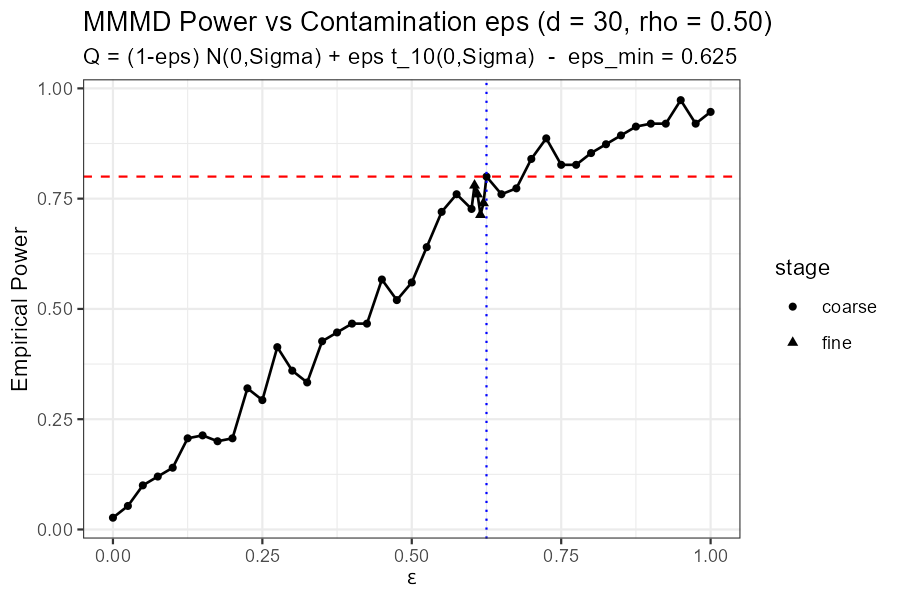
\includegraphics[width=0.78\textwidth]{figures/mmmd_epsilon_sensitivity.png}
\caption{$\varepsilon$-contamination sensitivity. $P=\mathcal{N}(0,\Sigma)$, $Q=(1-\varepsilon)\mathcal{N}(0,\Sigma)+\varepsilon\cdot t_{10}(0,\Sigma)$. GEXP kernel, $r=5$, $n=100$. Power reaches 0.80 at $\varepsilon=0.625$.}
\label{fig:eps-sensitivity}
\end{figure}

\subsection{Variance-scale sensitivity}

Figure~\ref{fig:var-sensitivity} and Table~\ref{tab:var-sensitivity} examine the minimum detectable covariance scaling. Under $P=\mathcal{N}(0,\Sigma_0)$ and $Q=\mathcal{N}(0,k\cdot\Sigma_0)$, the parameter $k>1$ controls the magnitude of the covariance inflation in the second population. All three MMMD kernel families (Mixed, Gauss, and LAP) detect $k_{\min}=1.25$ at power $\geq 0.80$, meaning a 25\% inflation in the overall covariance scale is sufficient for reliable detection. In contrast, the single-kernel Gaussian MMD requires $k_{\min}=1.40$, a 40\% inflation, to reach the same power threshold.

The gap is most striking at small effect sizes. At $k=1.20$ (a 20\% covariance increase), the multi-kernel methods achieve power 0.71--0.79, while the single-kernel baseline remains at 0.18. This roughly four-fold difference illustrates the practical value of multi-kernel aggregation: when the distributional shift is subtle relative to sampling variability, combining several bandwidths provides a more sensitive aggregate statistic than any single bandwidth can offer alone. The three MMMD variants perform similarly in this setting, suggesting that the aggregation mechanism (Mahalanobis weighting), rather than the specific kernel family, drives the gain over the single-kernel test.

\begin{figure}[H]
\centering
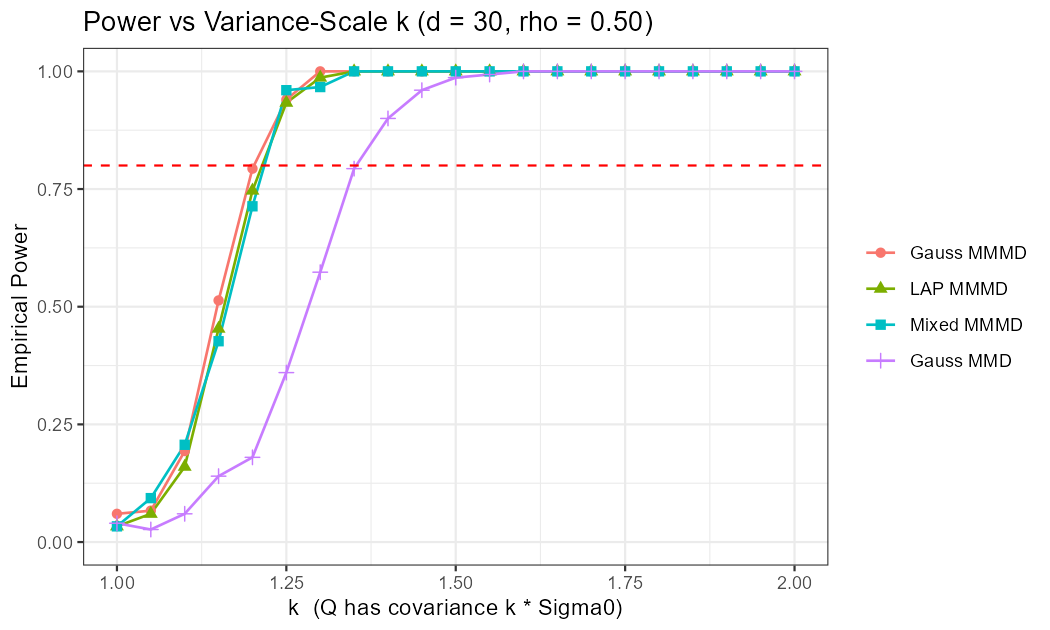
\includegraphics[width=0.78\textwidth]{figures/mmmd_variance_sensitivity.png}
\caption{Variance-scale sensitivity. $P=\mathcal{N}(0,\Sigma_0)$, $Q=\mathcal{N}(0,k\cdot\Sigma_0)$. Mixed MMMD detects $k_{\min}=1.25$; single-kernel Gauss MMD requires $k_{\min}=1.40$.}
\label{fig:var-sensitivity}
\end{figure}

\begin{table}[H]
\centering
\caption{Variance-scale sensitivity: endpoint power and detection thresholds.}
\label{tab:var-sensitivity}
\begin{tabular}{lcc}
\toprule
Method & $k_{\min}$ (power $\geq 0.80$) & Power at $k=1.20$ \\
\midrule
Mixed MMMD  & 1.25 & 0.71 \\
Gauss MMMD  & 1.25 & 0.79 \\
LAP MMMD    & 1.25 & 0.75 \\
Gauss MMD (single) & 1.40 & 0.18 \\
\bottomrule
\end{tabular}
\end{table}

\subsection{Type-I error calibration and ROC analysis}

Table~\ref{tab:type1} reports empirical Type-I error rates for the three kernel families at bandwidth counts $r\in\{3,5,10\}$. At moderate bandwidth counts ($r=3$ and $r=5$), all families are well-calibrated near the nominal $\alpha=0.05$. At $r=10$, a divergence appears: GEXP inflates to 0.120, exceeding twice the nominal rate; MIXED rises to 0.070; while LAP remains stable at 0.050. This pattern is consistent with the geometry of the kernel families. Gaussian kernels with close bandwidths produce near-identical Gram matrices, making the empirical covariance $\hat{\Sigma}$ nearly singular even after the paper's ridge regularization. Laplace kernels, with their heavier tails in the feature space, maintain better separation between neighbouring bandwidths, so the covariance estimate remains better conditioned at larger $r$.

Figure~\ref{fig:roc} provides the ROC perspective at a fixed variance-shift alternative ($k=1.25$). All three families trace similar ROC curves with false-positive rates (FPR) near 0.05 and true-positive rates (TPR) between 0.435 and 0.500. The fact that TPR values are comparable despite the Type-I differences at large $r$ is informative: the calibration advantage of LAP at $r=10$ does not translate into a substantial power advantage when the alternative is strong enough to be detected by any of the families. The practical guidance is to keep GEXP at $r\leq 5$ for well-calibrated inference, and to prefer LAP when a larger bandwidth bank is desired.

\begin{figure}[H]
\centering
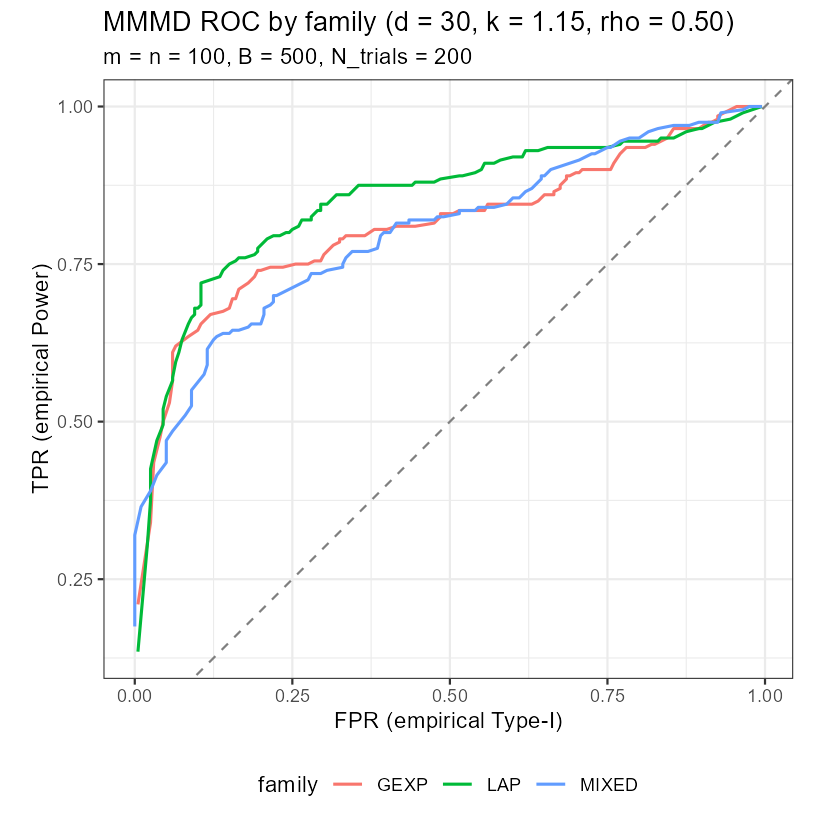
\includegraphics[width=0.78\textwidth]{figures/mmmd_roc_curves.png}
\caption{ROC curves for three kernel families at a fixed variance-shift alternative ($d=30$, $k=1.25$, $n=100$). All families maintain FPR $\approx 0.05$ with comparable TPR.}
\label{fig:roc}
\end{figure}

\begin{table}[H]
\centering
\caption{Type-I error across kernel families and bandwidth counts. Nominal level $\alpha=0.05$.}
\label{tab:type1}
\begin{tabular}{lccc}
\toprule
Kernel family & $r=3$ & $r=5$ & $r=10$ \\
\midrule
GEXP  & 0.020 & 0.055 & 0.120 \\
LAP   & 0.045 & 0.045 & 0.050 \\
MIXED & 0.050 & 0.050 & 0.070 \\
\bottomrule
\end{tabular}
\end{table}

\subsection{Graph-MMMD: construction, calibration, and skewness robustness}

The Graph-MMMD extension replaces the Euclidean kernel with a diffusion-based kernel constructed from the sample graph. A $k$-nearest-neighbor graph is built on the pooled sample $\mathcal{X}_m\cup\mathcal{Y}_n$, the normalized graph Laplacian $L$ is formed, and the heat kernel $K_t=\exp(-tL)$ generates a family of kernels indexed by the diffusion time $t$. This construction is appealing for biomedical applications where the natural geometry of the data may be non-Euclidean --- for instance, when samples lie on a low-dimensional manifold or exhibit cluster structure that Euclidean distances do not capture well.

Figure~\ref{fig:graph-type1} validates the Type-I error of Graph-MMMD under four null distributions that differ in their tail weight and asymmetry: Gaussian AR(1) ($\rho=0.5$), scaled Gaussian ($k=1.5$), skew-normal with shape $\alpha=5$, and multivariate Laplace. Empirical rejection rates are 0.027, 0.020, 0.020, and 0.033, respectively --- all well below the nominal 0.05 level. The method is not inflated by either heavy tails (Laplace) or asymmetry (skew-normal).

Figure~\ref{fig:skew-type1} provides a finer-grained skewness sweep. The skew-normal shape parameter $\alpha$ is mapped to standardized skewness via the known moment formulas, and $\alpha$ is solved numerically by \texttt{uniroot()} to hit six target skewness levels from 0.00 (symmetric) to 0.90 (strongly skewed). Across the full range, Type-I error stays between 0.020 and 0.053 with no systematic upward or downward trend. This stability is noteworthy because many parametric tests that assume symmetry can become liberal under skewed nulls; Graph-MMMD shows no such sensitivity. The absence of monotonic drift also suggests that the graph Laplacian eigenstructure is not systematically altered by skewness in a way that biases the kernel-based statistic under $H_0$.

\begin{figure}[H]
\centering
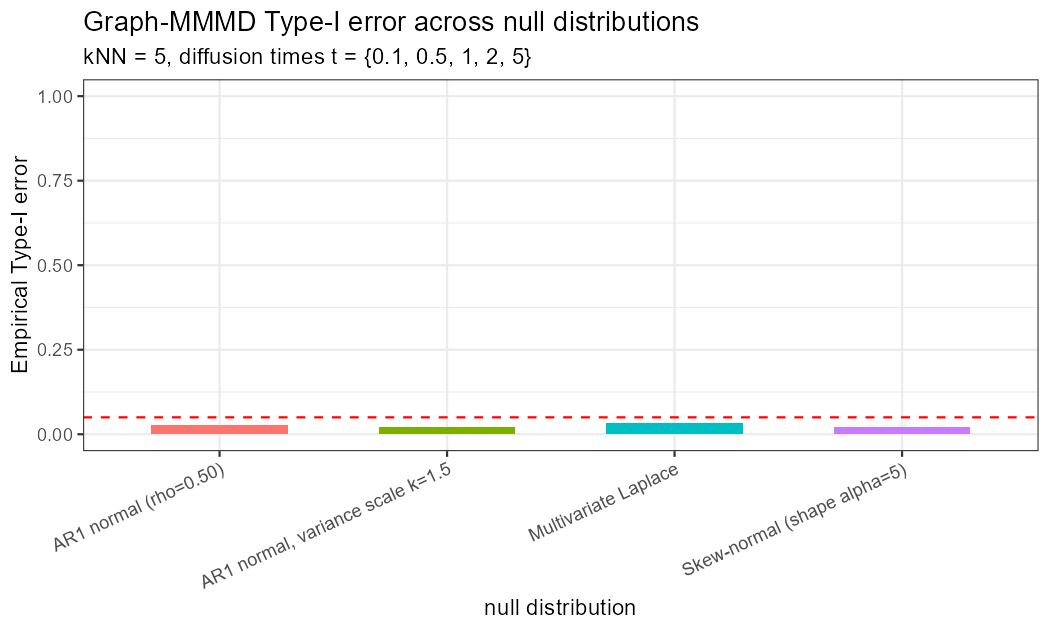
\includegraphics[width=0.78\textwidth]{figures/mmmd_graph_type1.png}
\caption{Graph-MMMD Type-I error under four null distributions. The graph-based kernel uses a $k$NN graph Laplacian with heat kernel $K_t=\exp(-tL)$. All rejection rates are at or below 0.053.}
\label{fig:graph-type1}
\end{figure}

\begin{figure}[H]
\centering
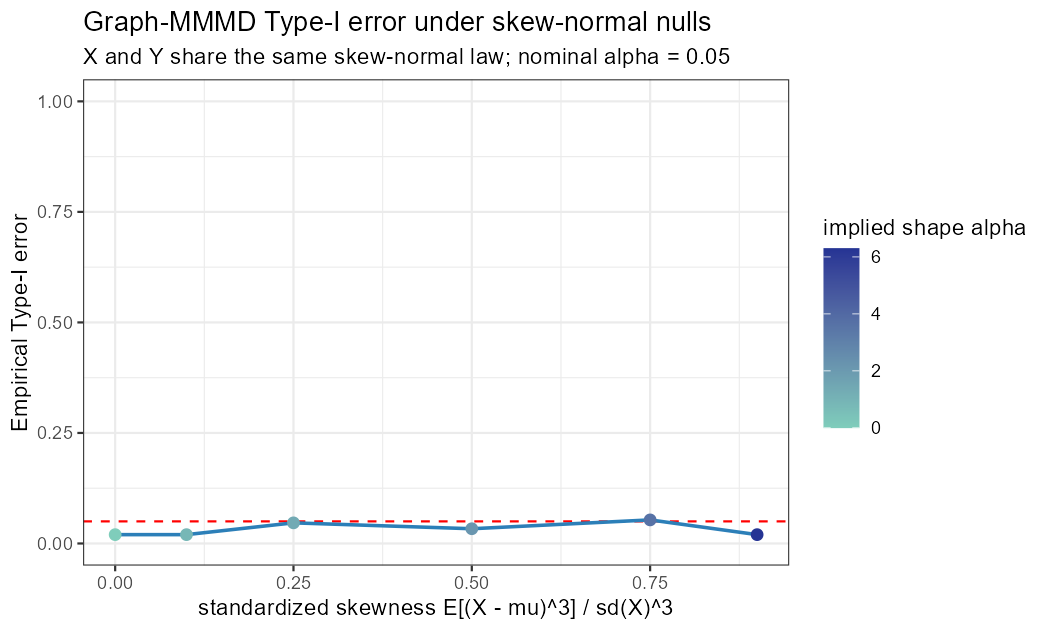
\includegraphics[width=0.78\textwidth]{figures/mmmd_skew_type1.png}
\caption{Graph-MMMD Type-I error across skewness levels (skew-normal distribution, shape parameter $\alpha$ mapped to standardized skewness). Type-I error remains $\leq 0.053$ up to standardized skewness 0.90.}
\label{fig:skew-type1}
\end{figure}

\subsection{Mixture distribution power reproduction}

Figure~\ref{fig:mixture} and Table~\ref{tab:mixture} reproduce the original paper's normal-$t$ mixture experiment (Fig.~2). The two populations are $P=(1-p)\mathcal{N}(0,\Sigma_0)+p\cdot t_{10}(0,\Sigma_0)$ and $Q=(1-p)\mathcal{N}(0,\Sigma_1)+p\cdot t_{10}(0,\Sigma_1)$ with $\Sigma_1=1.25\cdot\Sigma_0$, and the mixture proportion $p\in\{0,0.4,1.0\}$ controls how much of each sample is heavy-tailed. At $p=0$, the populations differ only through the 25\% covariance inflation, and Mixed MMMD achieves power 0.96 versus 0.46 for the single-kernel benchmark. At $p=0.4$, the gap narrows slightly to 0.80 versus 0.31. At $p=1.0$ (both populations are pure $t_{10}$), the power drops for all methods but the multi-kernel advantage persists: 0.58 versus 0.35.

Two patterns are worth noting. First, power decreases monotonically with $p$ for all methods, because the $t_{10}$ tails inject more variance into both samples and make the covariance difference harder to isolate. Second, the relative advantage of MMMD over the single-kernel test is roughly stable (2--5$\times$) across all three $p$ levels, confirming that the benefit of multi-kernel aggregation is not specific to a particular mixture proportion. This reproduction anchors our numerical extensions to the original paper's Figure~2 and confirms that our R implementation recovers the expected qualitative patterns.

\begin{figure}[H]
\centering
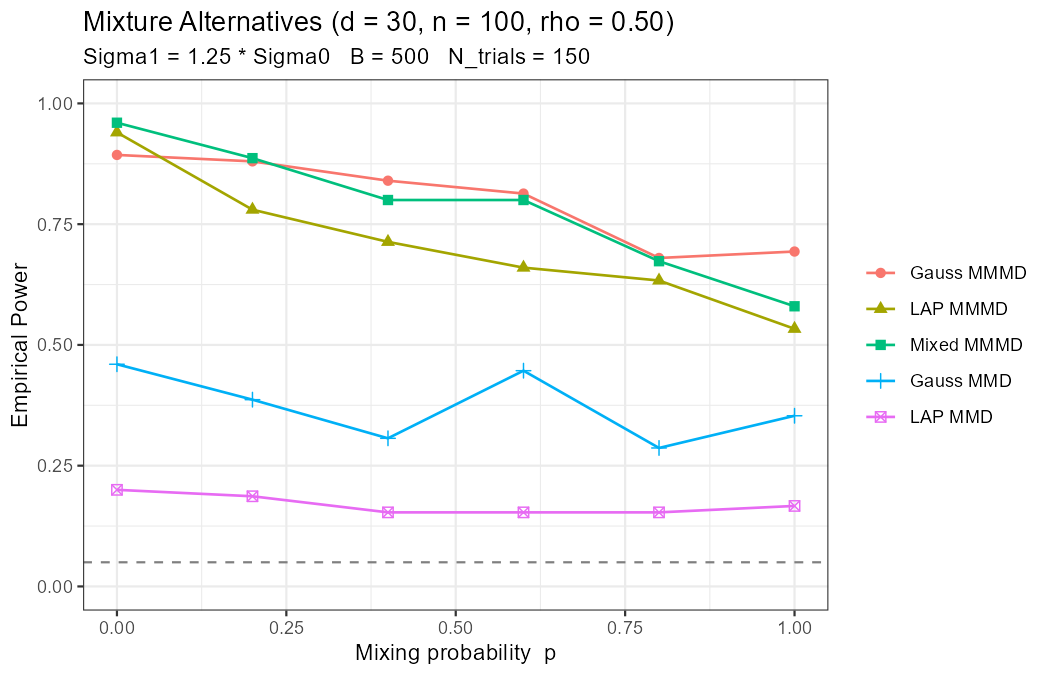
\includegraphics[width=0.78\textwidth]{figures/mmmd_fig2_mixture.png}
\caption{Reproduction of the original paper's Fig.~2: power under a normal-$t$ mixture alternative. $\Sigma_1=1.25\cdot\Sigma_0$, $\nu=10$. MMMD methods achieve 2--5$\times$ the power of single-kernel Gauss MMD.}
\label{fig:mixture}
\end{figure}

\begin{table}[H]
\centering
\caption{Mixture-distribution power: $P=(1-p)\mathcal{N}(0,\Sigma_0)+p\cdot t_{10}(0,\Sigma_0)$, $Q=(1-p)\mathcal{N}(0,\Sigma_1)+p\cdot t_{10}(0,\Sigma_1)$ with $\Sigma_1=1.25\cdot\Sigma_0$.}
\label{tab:mixture}
\begin{tabular}{lcccc}
\toprule
$p$ & MMMD-Mix & MMMD-Gauss & MMMD-LAP & MMD-Gauss \\
\midrule
0.0 & 0.96 & 0.89 & 0.94 & 0.46 \\
0.4 & 0.80 & 0.84 & 0.71 & 0.31 \\
1.0 & 0.58 & 0.69 & 0.53 & 0.35 \\
\bottomrule
\end{tabular}
\end{table}

Overall, these numerical extensions show that the Mahalanobis aggregation strategy generalizes well beyond the Gaussian mean-shift and variance-shift settings studied in the original paper. The multi-kernel advantage is most pronounced when the distributional difference is small relative to the noise, and the calibration properties are generally well-behaved provided the bandwidth count is kept moderate or the LAP family is used. The graph-based variant further demonstrates that the MMMD framework can accommodate non-Euclidean kernel constructions without compromising Type-I error control.

\clearpage
\section{Detailed CNN-MMMD methods and diagnostics}
\label{app:dechao-cnn-mmmd}
\captionsetup[figure]{font=small,skip=4pt}
\captionsetup[table]{font=small,skip=4pt}

This appendix documents the experimental design and calculations underlying Section~\ref{sec:cnn-mmmd}. It separates the main testing pipeline from the later diagnostic analyses so that the source of each reported number is explicit.

\subsection{Data separation, run sizes, and leakage control}

For MNIST, the CNN was trained on the training split and all MMMD evaluations used held-out images. For PathMNIST, the official training split (the source domain) was divided stratifiably into a CNN-training pool and a source-holdout pool. The CNN was trained on all nine tissue labels using only the CNN-training pool; the official validation split was used for checkpoint selection. The source-holdout pool and the official test split (the external domain) were reserved for two-sample testing. Thus neither group in the formal source-vs-external test was used to fit the CNN.

Formal PathMNIST power and internal-null analyses used 10 outer repetitions, 500 independent tests per outer repetition, and 500 multiplier-bootstrap draws per test, giving 5000 tests per method and sample-size cell. The semantic/residual robustness and label-8 dissection experiments used 10 outer repetitions, 20 inner tests, and 500 bootstrap draws; linear domain-axis analyses were repeated 20 times over train/holdout splits. Sampling was without replacement within a test, although different repeated tests could reuse observations.

\begin{table}[H]
\centering
\caption{Questions addressed by the CNN-MMMD experimental sequence.}
\label{tab:app-dechao-ledger}
\small
\setlength{\tabcolsep}{5pt}
\begin{tabular}{>{\raggedright\arraybackslash}p{0.22\textwidth}>{\raggedright\arraybackslash}p{0.69\textwidth}}
\toprule
Stage & Experimental role \\
\midrule
MNIST validation & Compare raw pixels and CNN representations under additive noise and check matched-null calibration. \\
PathMNIST class mixture & Test a controlled tissue-composition alternative, \texttt{mix635} versus \texttt{mix835}, with a matched \texttt{mix635} null. \\
Same-label center shift & Compare source-holdout and external images within labels 6 and 8, together with source-internal and external-internal nulls. \\
Semantic/residual analysis & Separate FC-128 directions used by the classifier from its orthogonal residual complement. \\
Residual robustness & Match effective dimension, vary residual PCA dimension, and check bootstrap sensitivity. \\
Color/stain analyses & Explain the residual domain score with RGB summaries, test color summaries directly, and rerun residual MMMD after color matching. \\
\bottomrule
\end{tabular}
\end{table}

\subsection{CNN features and MMMD variants}

The CNN feature hierarchy used in these image experiments came from two convolutional blocks followed by global average pooling, a 128-dimensional fully connected layer, and a final linear classifier. The extracted features were a 32-dimensional shallow pooled feature, a 64-dimensional intermediate pooled feature, and the 128-dimensional penultimate feature (FC-128). Raw 28-by-28 RGB images gave 2352 pixel coordinates in the PathMNIST experiments.

Four principal tests were compared. Raw-pixel Gaussian-5 and FC-128 Gaussian-5 each used five Gaussian bandwidths. The multilayer single-Gaussian test used one Gaussian kernel on each of the three CNN feature levels, producing three MMD components. Multilayer Gaussian-15 used five bandwidths at each feature level, producing 15 components. The same sampled image indices were used across representations within a repeated test. All component vectors were combined by the MMMD statistic in Section~2.

\begin{figure}[H]
\centering
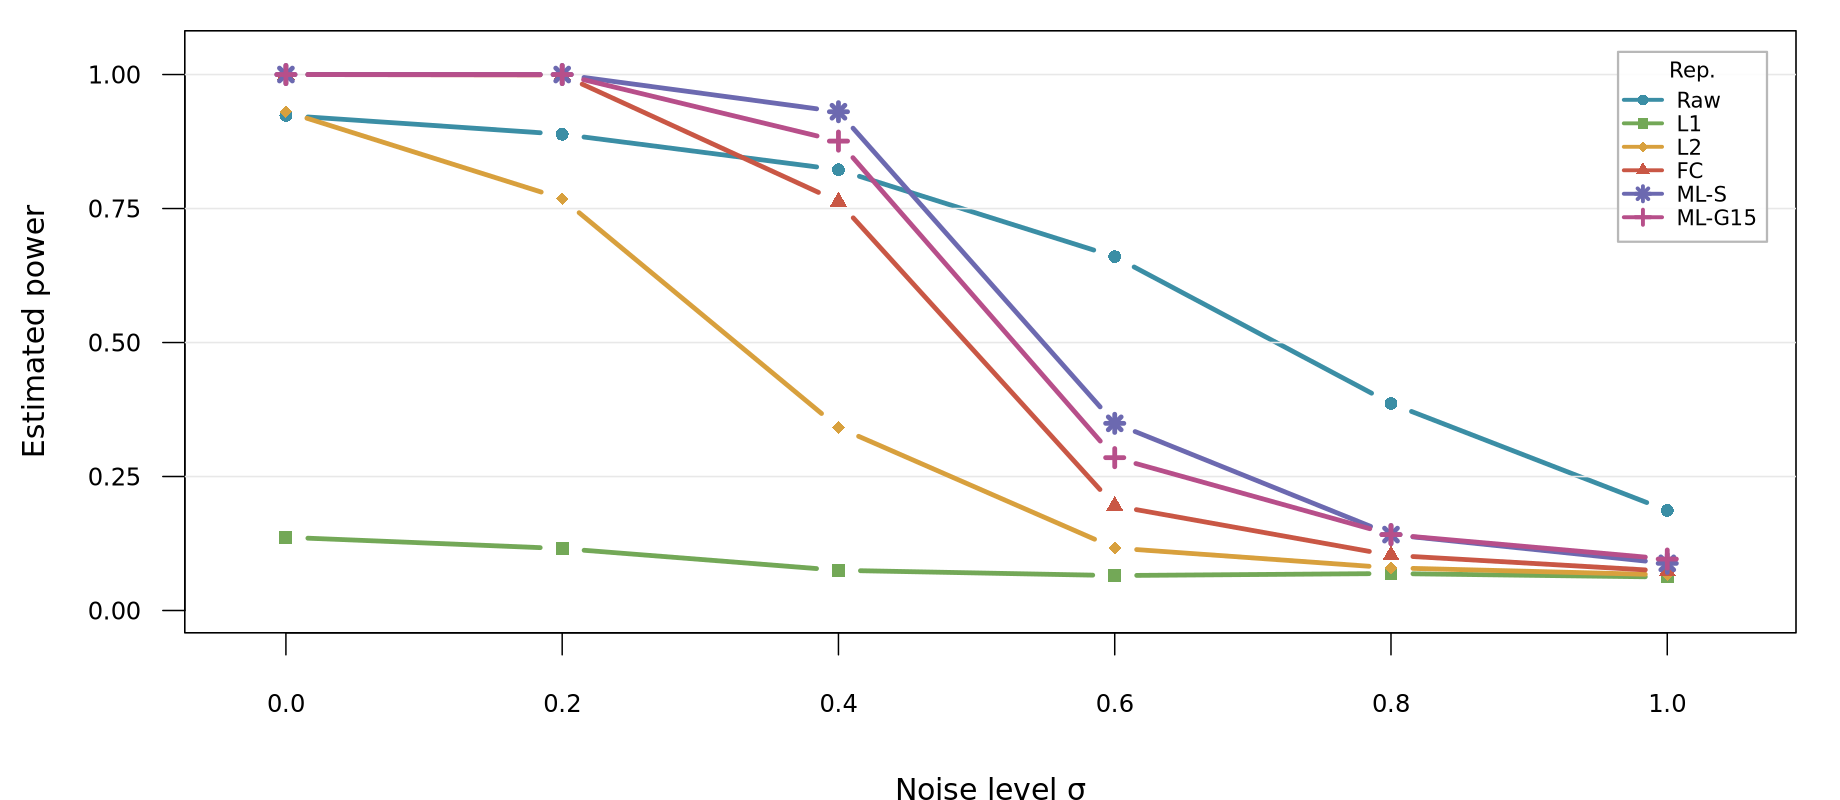
\includegraphics[width=0.82\textwidth]{figures/dechao_mnist_cnn_power}\\[-2pt]
\textbf{(a)} Power across additive-noise levels

\vspace{6pt}
\centering
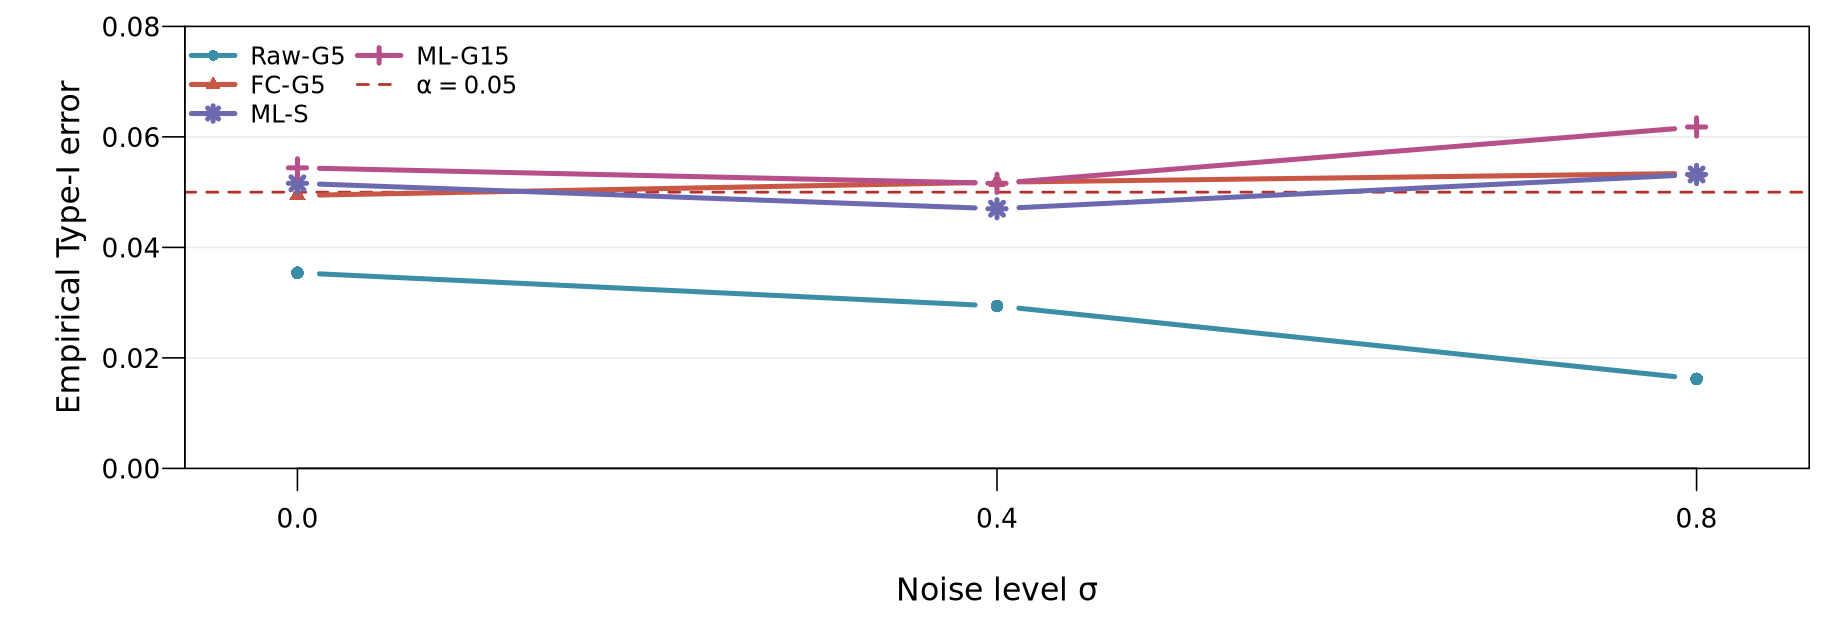
\includegraphics[width=0.82\textwidth]{figures/dechao_mnist_type1_all_methods.png}\\[-2pt]
\textbf{(b)} Matched-null Type-I error for \texttt{set123} vs \texttt{set123}
\caption{MNIST validation of the representation-assisted MMMD pipeline. In panel (a), L1 and L2 denote single-layer Gaussian-5 tests on the shallow and intermediate CNN features. In panel (b), Raw-G5 denotes raw-pixel Gaussian-5, FC-G5 denotes FC-128 Gaussian-5, ML-S denotes multilayer single-Gaussian, and ML-G15 denotes multilayer Gaussian-15. The dashed line marks the nominal $\alpha=0.05$ level.}
\label{fig:app-dechao-mnist-validation}
\end{figure}

\subsection{PathMNIST alternatives and internal-null checks}

The class-mixture alternative compared observations drawn from labels $\{6,3,5\}$ with observations drawn from labels $\{8,3,5\}$ using the project mixture sampler. The matched null compared two independently sampled \texttt{mix635} groups. The main sample-size grid was $n\in\{30,60,90,120,150\}$ per group.

For center shift and a fixed tissue label $c\in\{6,8\}$, the alternative was
\[
X\sim \text{source-holdout}(c),\qquad Y\sim \text{external}(c).
\]
Two internal nulls were evaluated separately: both groups sampled from source-holdout$(c)$, and both groups sampled from external$(c)$. The center-shift grid was $n\in\{20,30,50,80,100\}$ where feasible. When a single conservative null reference is displayed, ``max $H_0$'' denotes the larger of the source-internal and external-internal rejection rates.

\begin{figure}[H]
\centering
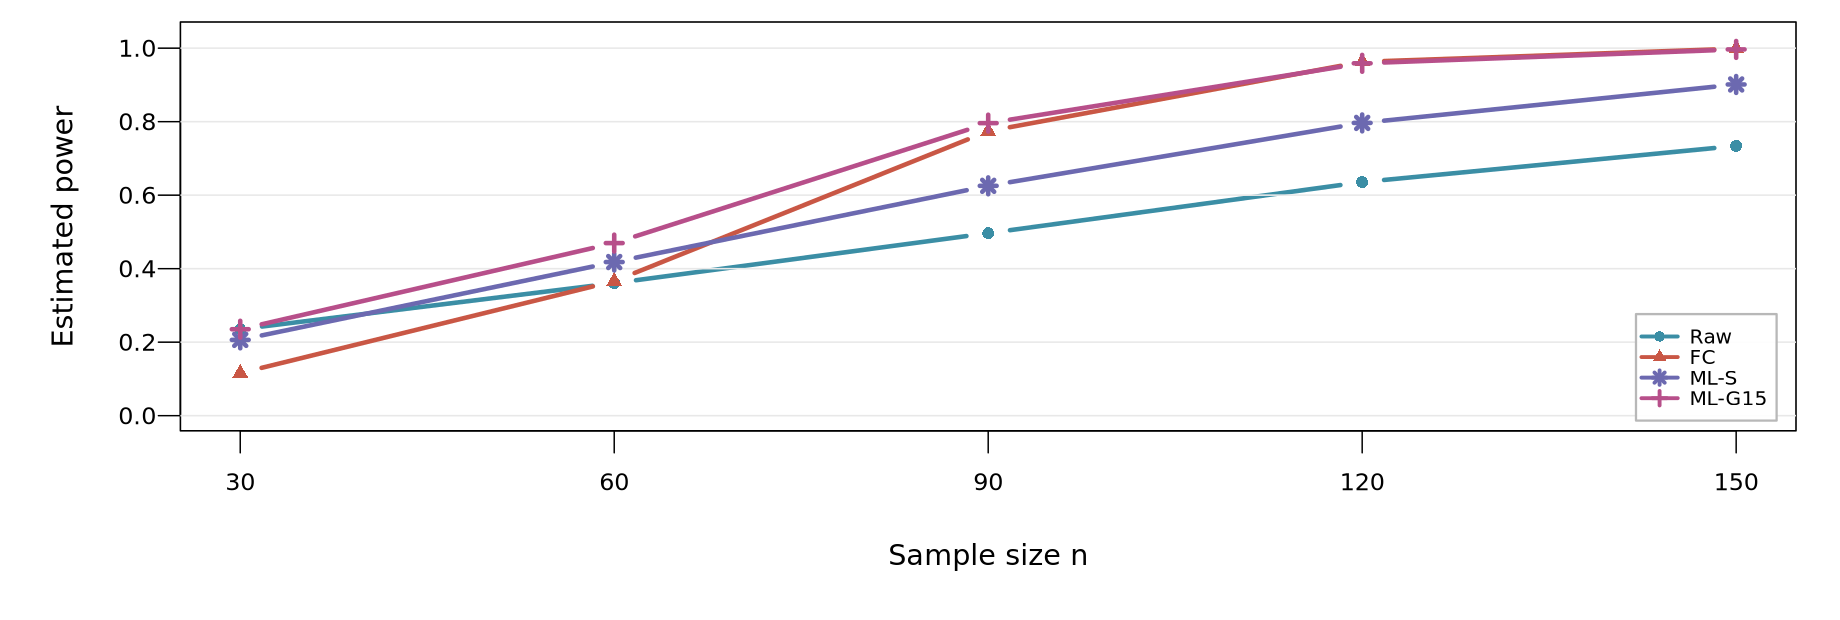
\includegraphics[width=0.82\textwidth]{figures/dechao_pathmnist_class_mixture_power.png}\\[-2pt]
\textbf{(a)} Class-mixture power

\vspace{7pt}
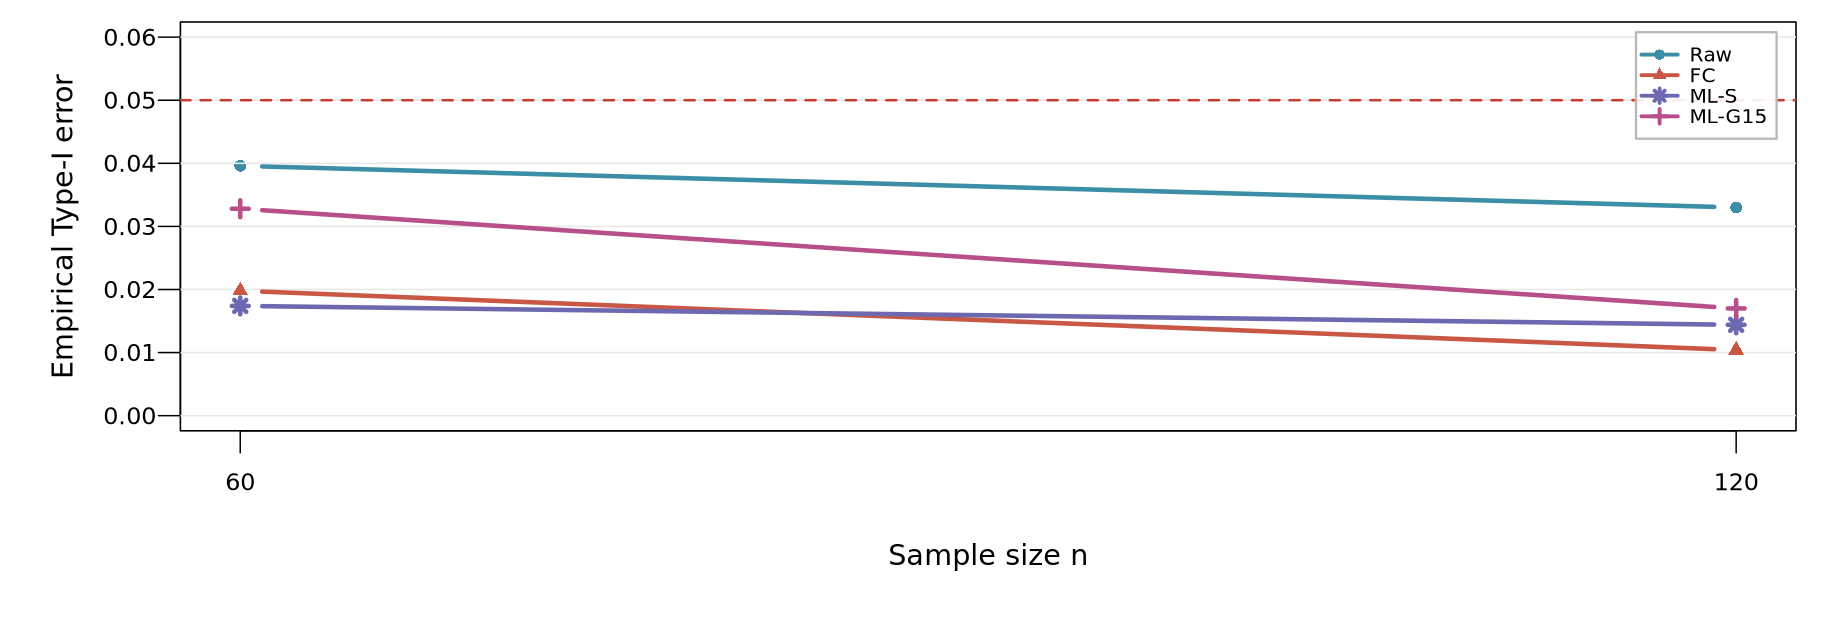
\includegraphics[width=0.82\textwidth]{figures/dechao_pathmnist_class_type1_zoom.png}\\[-2pt]
\textbf{(b)} Matched-null Type-I error
\caption{PathMNIST class-mixture alternative and matched-null calibration.}
\label{fig:app-dechao-path-class}
\end{figure}

\begin{figure}[H]
\centering
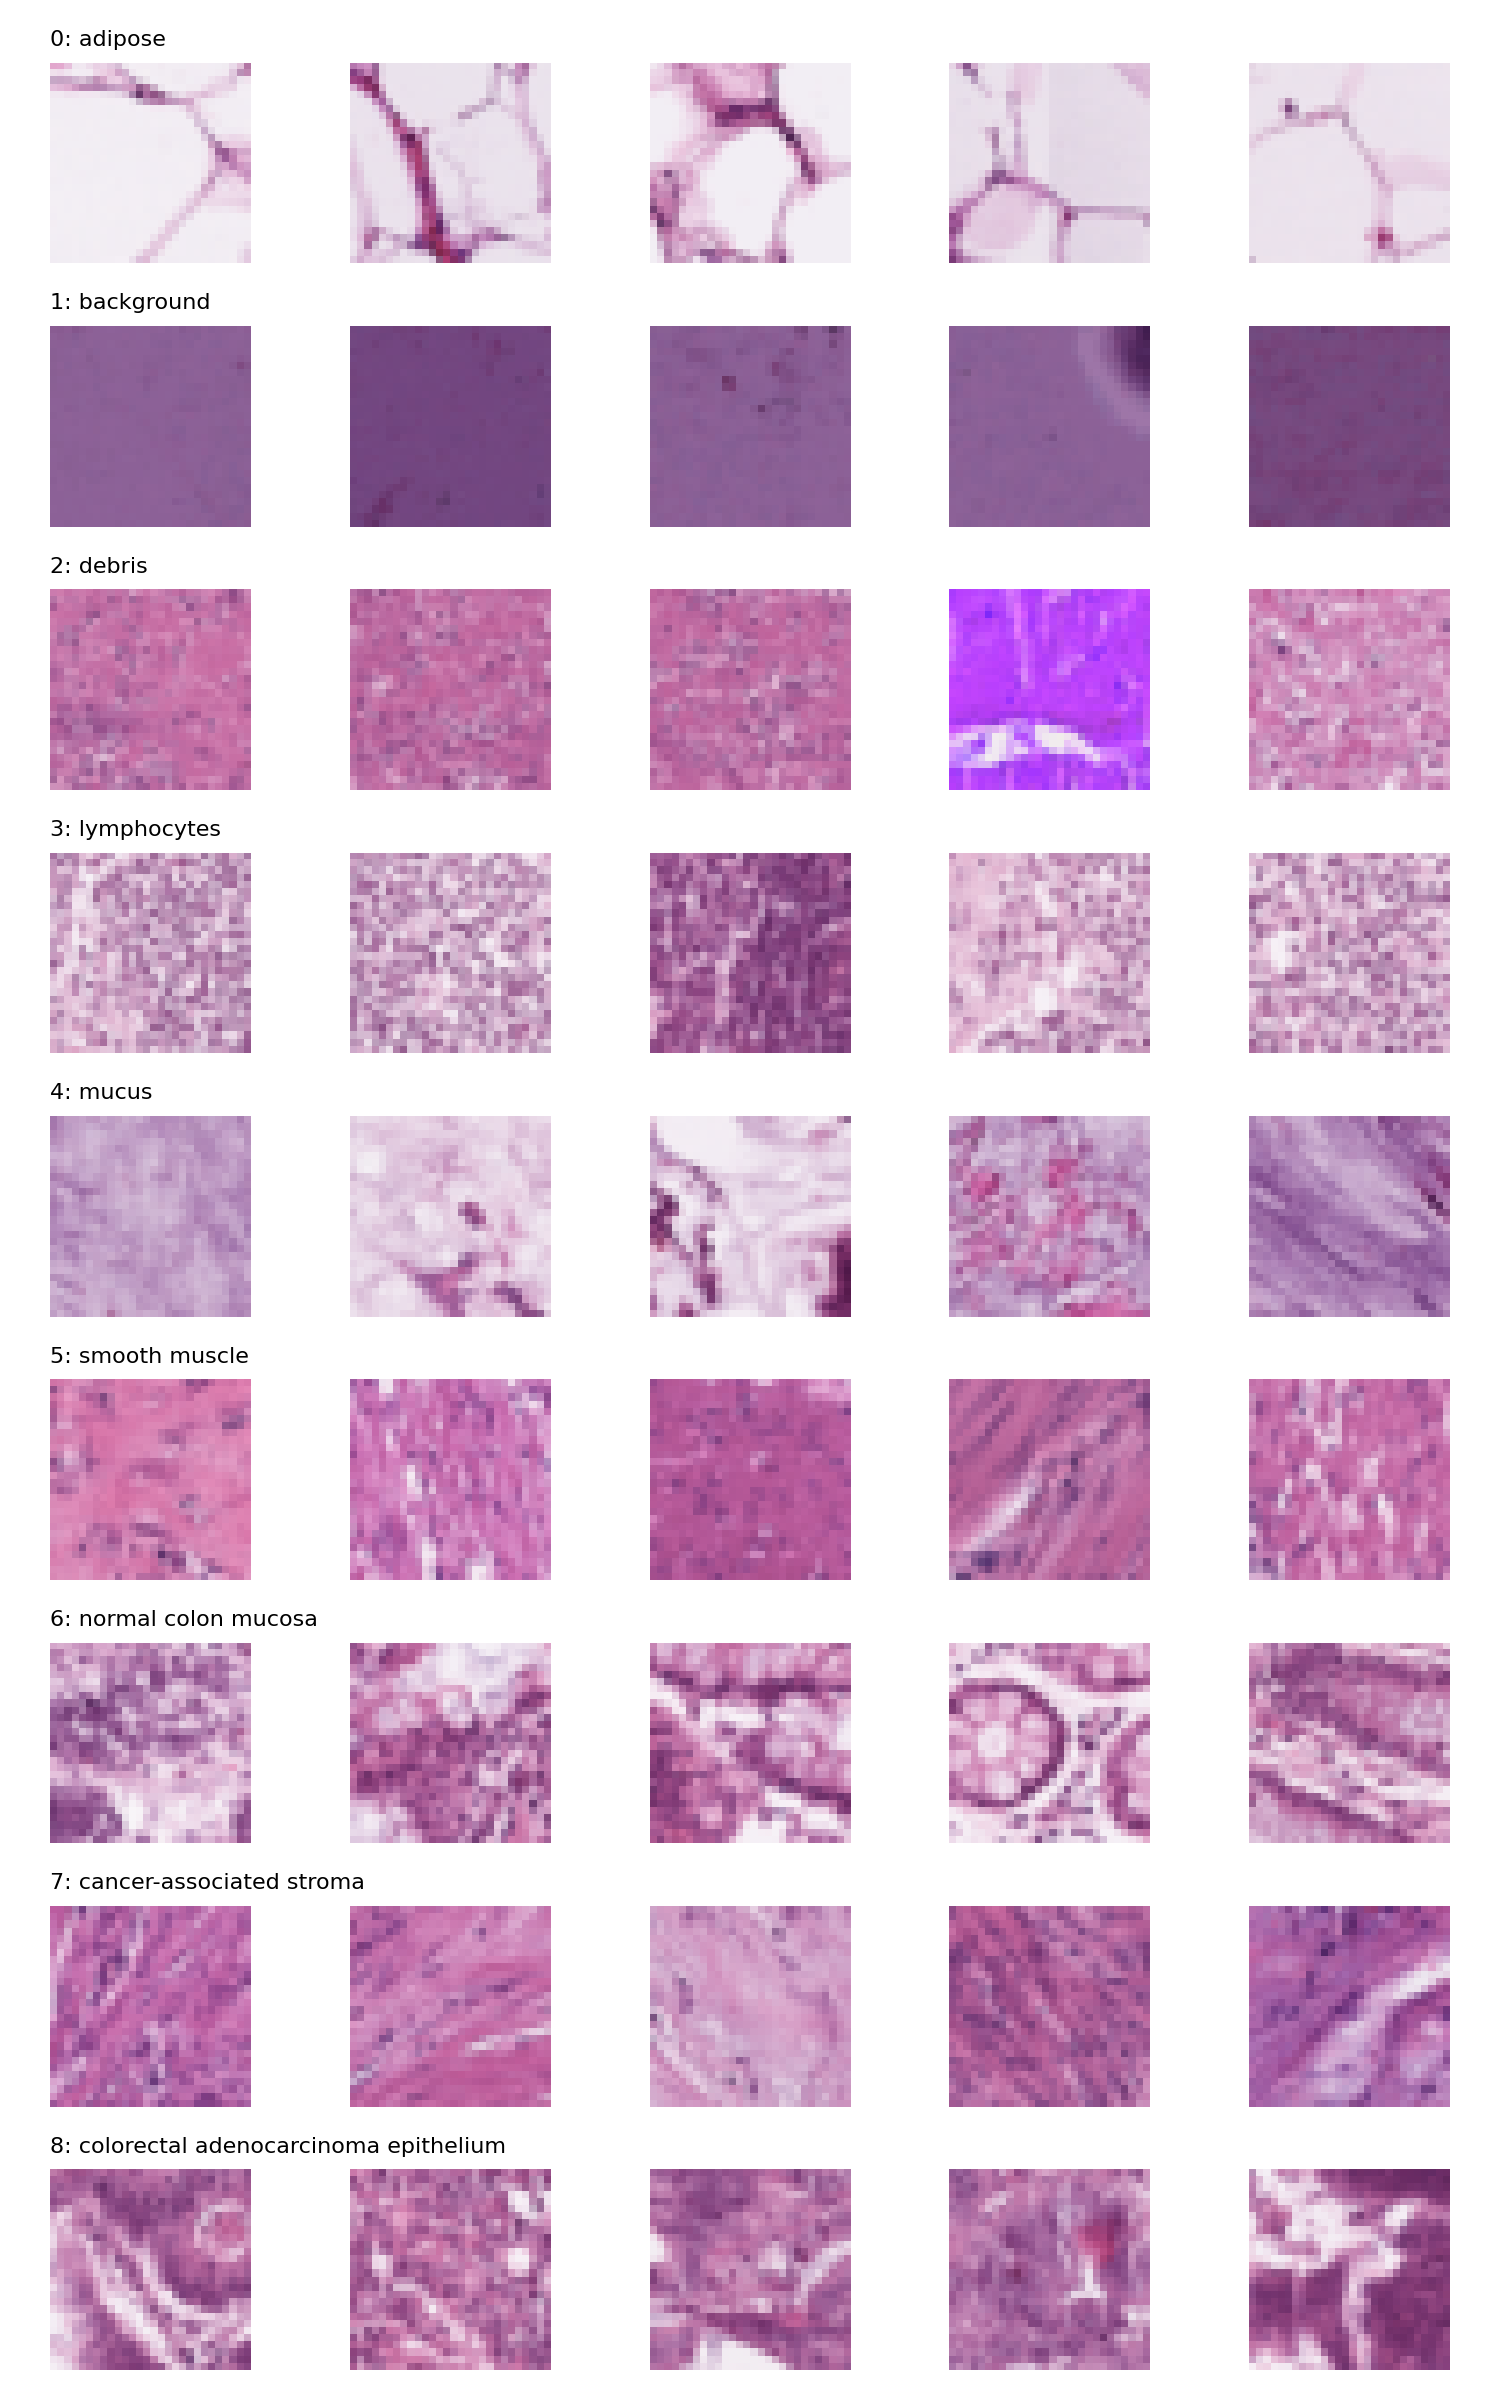
\includegraphics[width=0.95\textwidth,trim=0 0 0 380,clip]{figures/dechao_pathmnist_examples.png}
\caption{Representative tissue classes used in the center-shift analysis.}
\label{fig:app-dechao-examples}
\end{figure}

\begin{figure}[H]
\centering
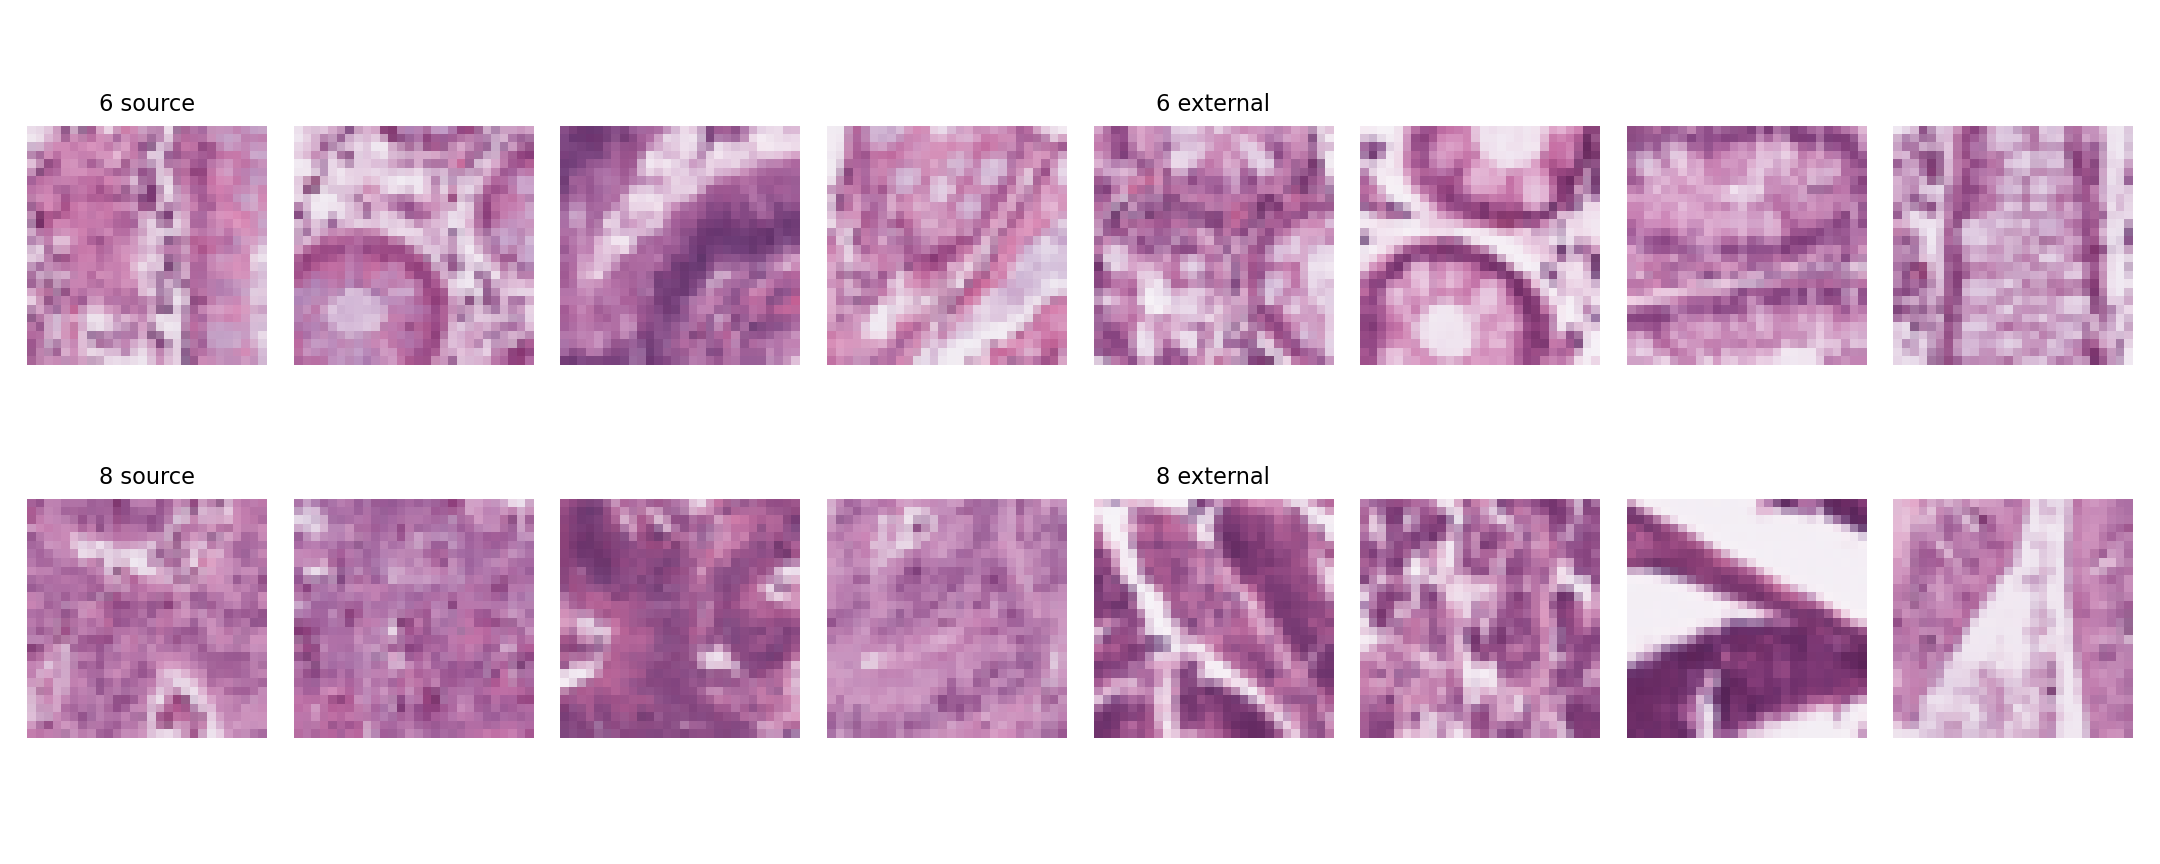
\includegraphics[width=0.95\textwidth]{figures/dechao_pathmnist_center_shift_examples.png}
\caption{Same-label source and external PathMNIST images for labels 6 and 8.}
\label{fig:app-dechao-center-examples}
\end{figure}

\begin{center}
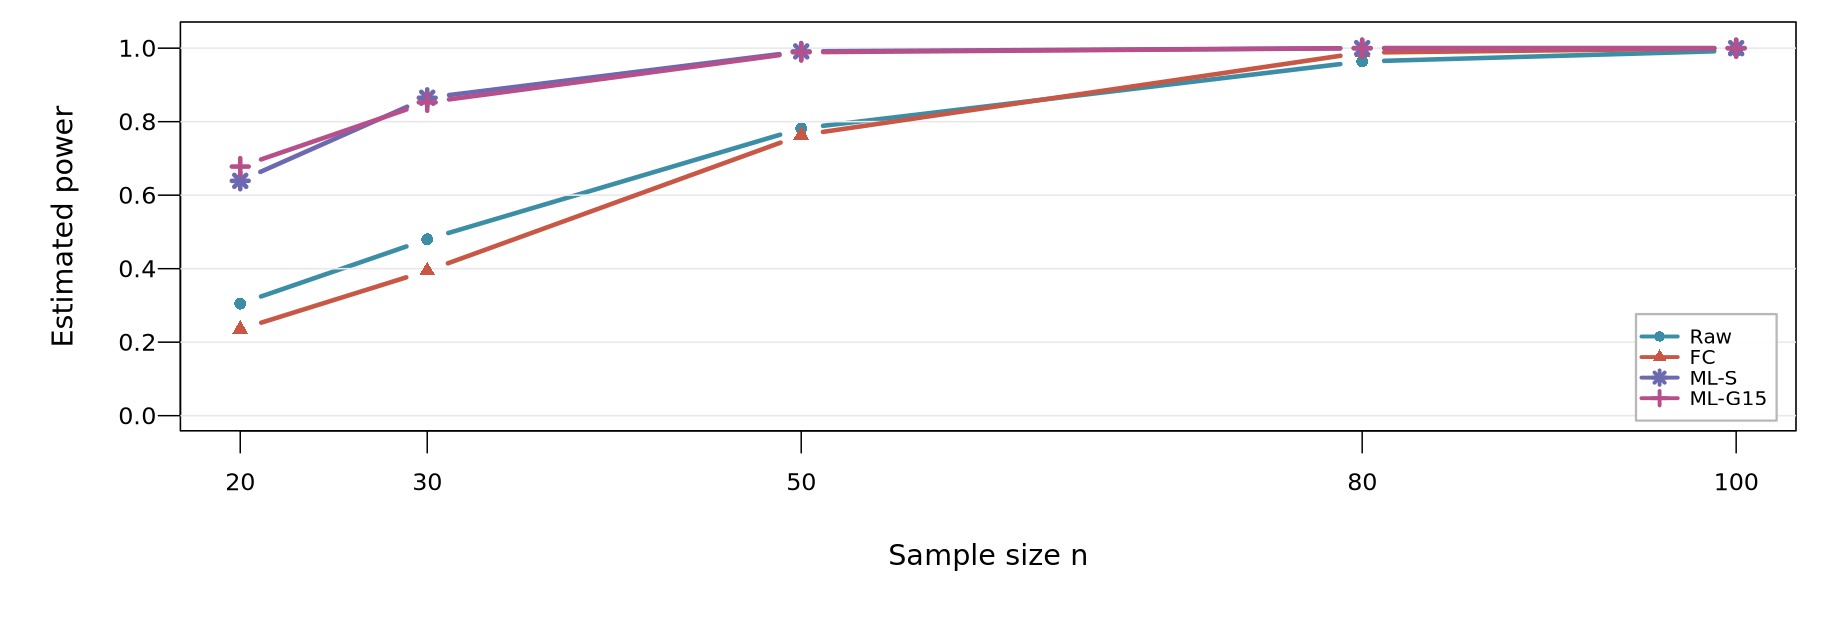
\includegraphics[width=0.95\textwidth]{figures/dechao_center_shift_power_label6.png}\\[-2pt]
\textbf{(a)} Label 6 power

\vspace{7pt}
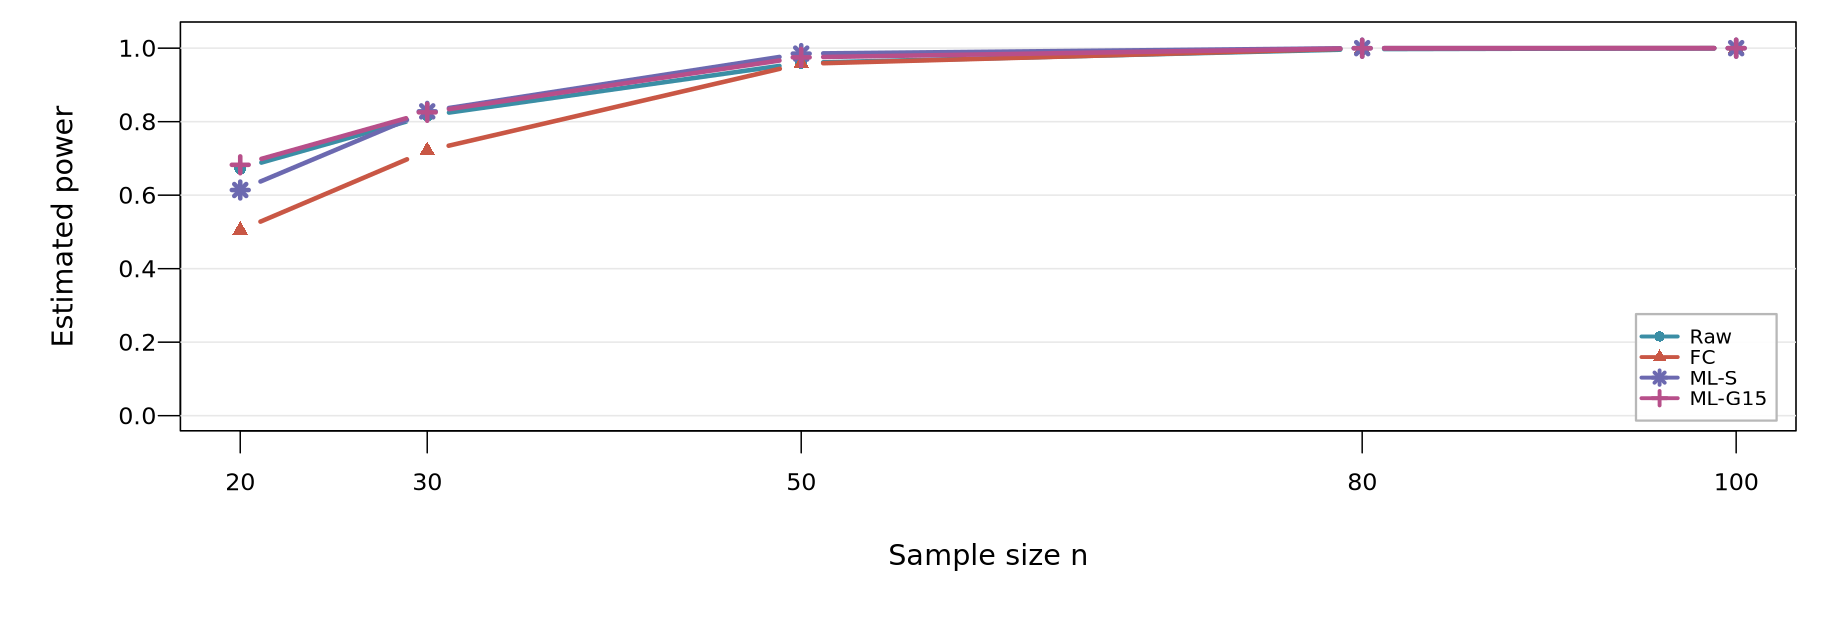
\includegraphics[width=0.95\textwidth]{figures/dechao_center_shift_power_label8.png}\\[-2pt]
\textbf{(b)} Label 8 power
\end{center}

\begin{figure}[H]
\centering
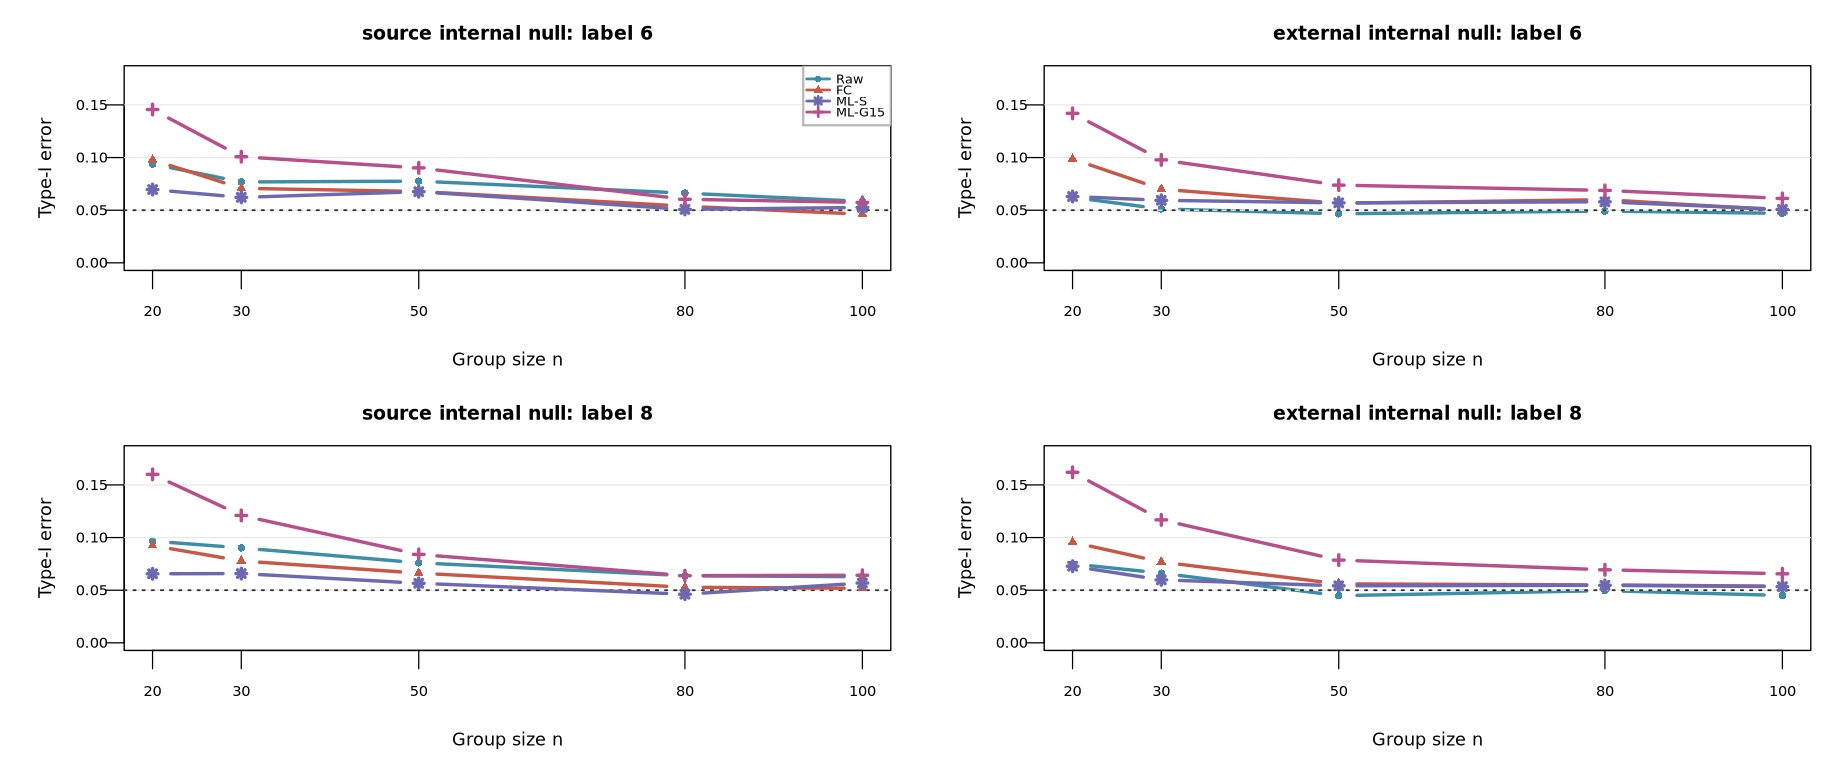
\includegraphics[width=0.95\textwidth]{figures/dechao_pathmnist_center_shift_type1.png}\\[-2pt]
\textbf{(c)} Source-internal and external-internal null checks
\caption{Same-label source-vs-external power and the corresponding internal-null references.}
\label{fig:app-dechao-center-results}
\end{figure}

\subsection{Centered semantic/residual decomposition}

Let $h_i\in\mathbb{R}^{128}$ be the FC-128 embedding and let the frozen classifier produce logits $Wh_i+b$, where $W\in\mathbb{R}^{9\times128}$. Softmax is invariant to adding the same constant to all nine logits, so the class-discriminative weight matrix was centered across classes:
\[
H_C=I_C-\frac{1}{C}\mathbf 1\mathbf 1^\top,\qquad W_c=H_CW=W-\mathbf 1\bar w^\top.
\]
The dimensions of $W$ and $W_c$ are both $9\times128$, but the rows of $W_c$ sum to zero and its rank is at most $C-1=8$. An orthonormal basis $V$ for $\operatorname{row}(W_c)$ was obtained by singular-value decomposition. The two components were
\[
h_{i,\mathrm{sem}}=VV^\top h_i,\qquad h_{i,\mathrm{res}}=h_i-h_{i,\mathrm{sem}}.
\]
Numerically, $W_ch_{i,\mathrm{res}}$ was zero up to floating-point tolerance. MMMD was then run separately on centered logits, $h_{\mathrm{sem}}$, $h_{\mathrm{res}}$, and the full embedding. No network parameters were changed during this analysis.

\begin{figure}[H]
\centering
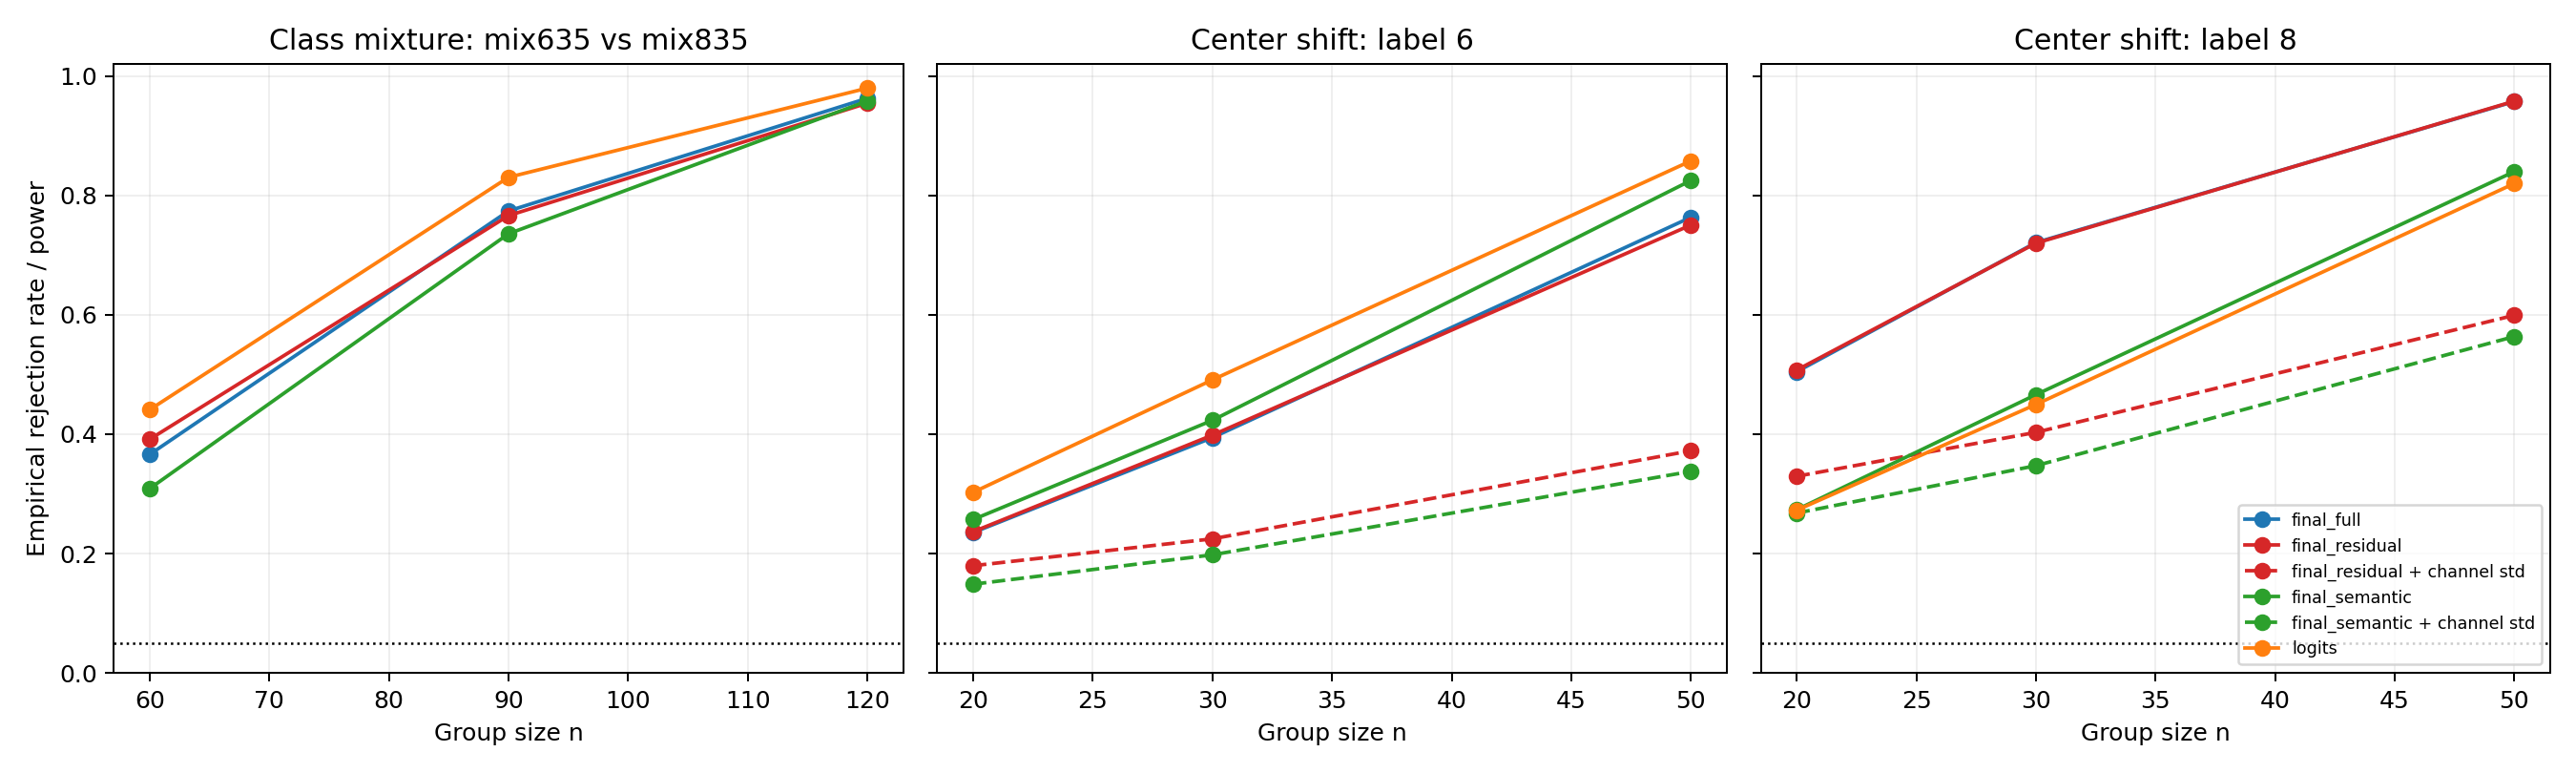
\includegraphics[width=0.88\textwidth]{figures/dechao_semantic_vs_residual_power.png}
\caption{MMMD rejection rates for classifier logits, centered semantic features, and residual features.}
\label{fig:app-dechao-semres-power}
\end{figure}

\subsection{Dimension matching, residual PCA, and calibration sensitivity}

Although $h_{\mathrm{sem}}$ and $h_{\mathrm{res}}$ are both stored as 128-dimensional vectors, their effective dimensions differ: $h_{\mathrm{sem}}$ lies in a rank-8 subspace, whereas the residual complement can contain roughly 120 directions. The dimension-matched control therefore projected residual features to eight dimensions in two ways. First, PCA was fitted on the pooled residual feature pool without using source/external labels and the leading eight scores were retained. Second, random orthonormal 8D projections were generated repeatedly; the reported random-8 result averages over 20 projections.

A separate intrinsic-dimension analysis used a label-8-specific PCA basis and retained $k\in\{1,2,4,8,16,32\}$ components. Consequently, the 8D value in the dimension-matched control (0.965) and the $k=8$ value in the intrinsic-dimension curve (0.970) use different PCA bases and independent repeated tests. The difference of 0.005 corresponds to one rejection among 200 tests. Multiplier bootstrap remained the primary calibration; permutation cutoffs were computed only as a sensitivity check in selected cells.

\begin{figure}[H]
\centering
\begin{minipage}[t]{0.49\textwidth}
\centering
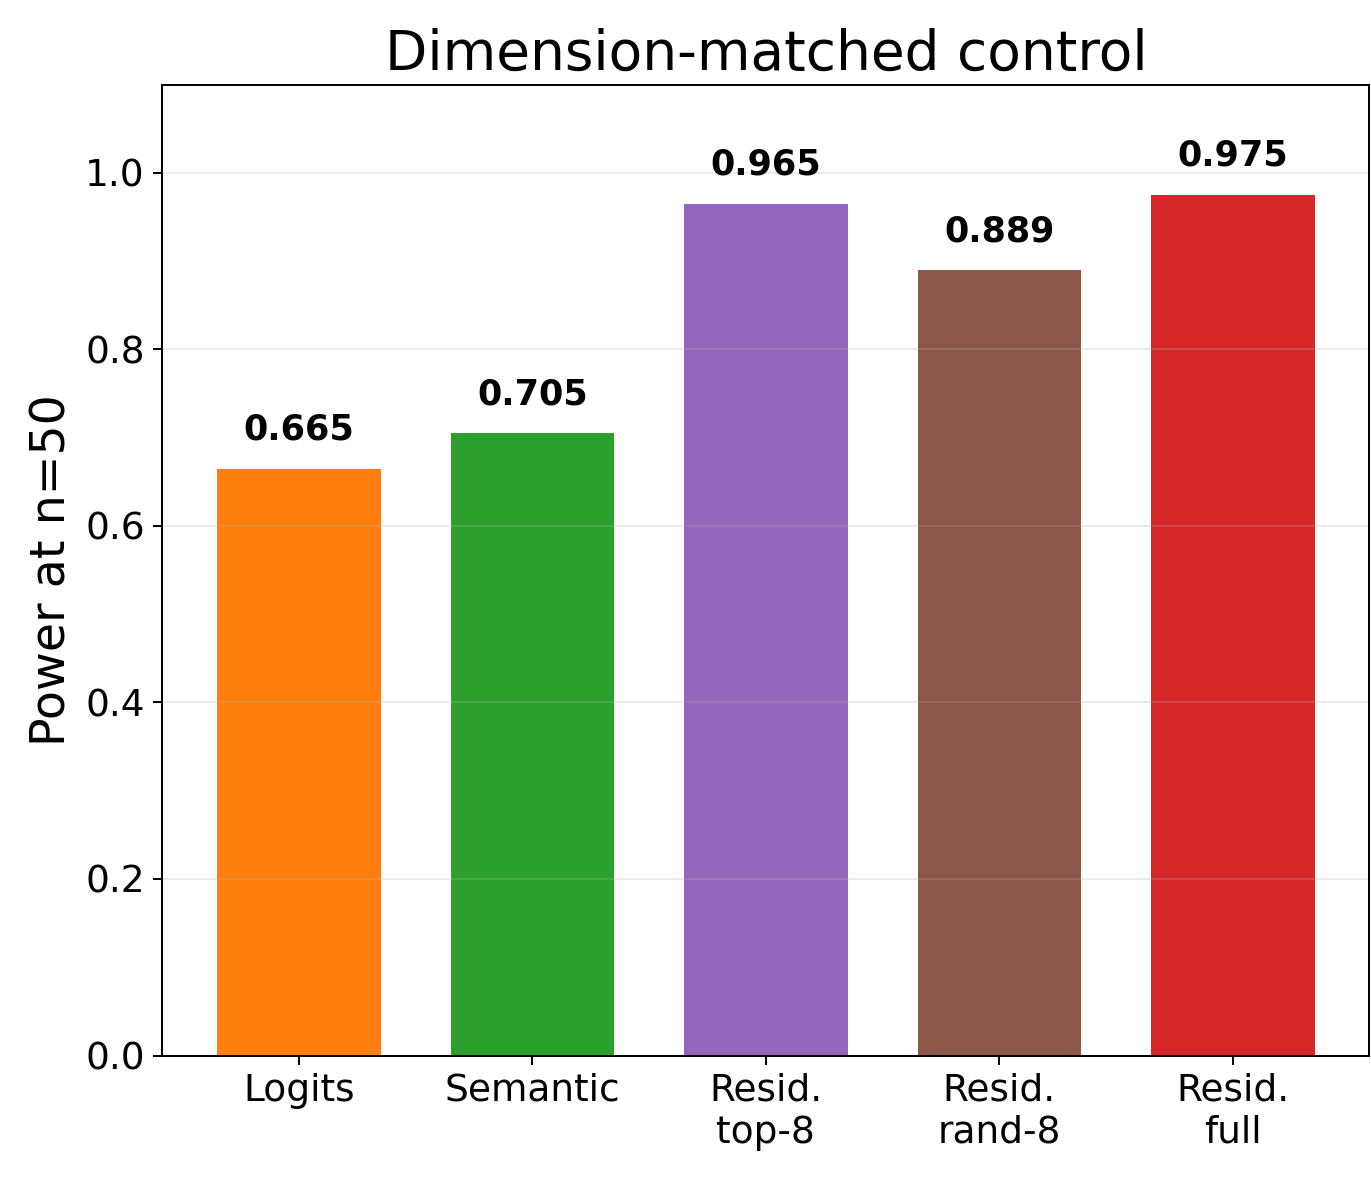
\includegraphics[width=\linewidth]{figures/dechao_label8_residual_dimension_matched.png}\\[-2pt]
\textbf{(a)} Dimension-matched comparison at $n=50$
\end{minipage}\hfill
\begin{minipage}[t]{0.49\textwidth}
\centering
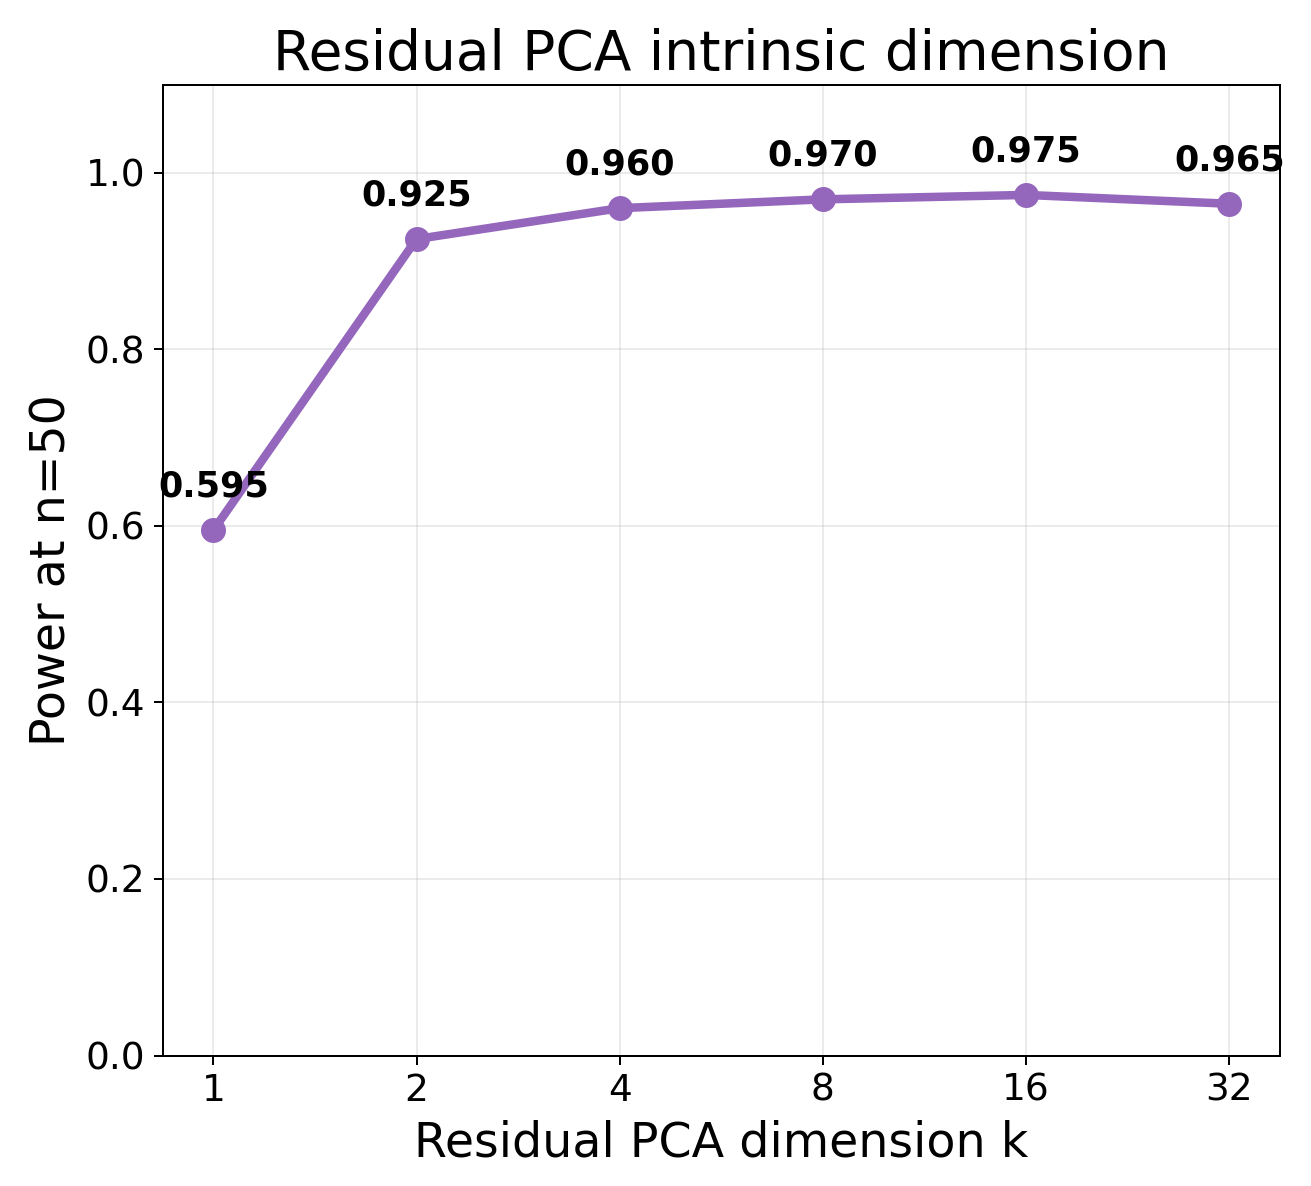
\includegraphics[width=\linewidth]{figures/dechao_label8_residual_pca_dimension.png}\\[-2pt]
\textbf{(b)} Label-8-specific residual PCA sweep
\end{minipage}
\caption{Residual dimension controls. The residual signal persists at eight dimensions and is largely captured by the first two to four label-8-specific PCs.}
\label{fig:app-dechao-residual-dimension}
\end{figure}

\begin{figure}[H]
\centering
\begin{minipage}[t]{0.49\textwidth}
\centering
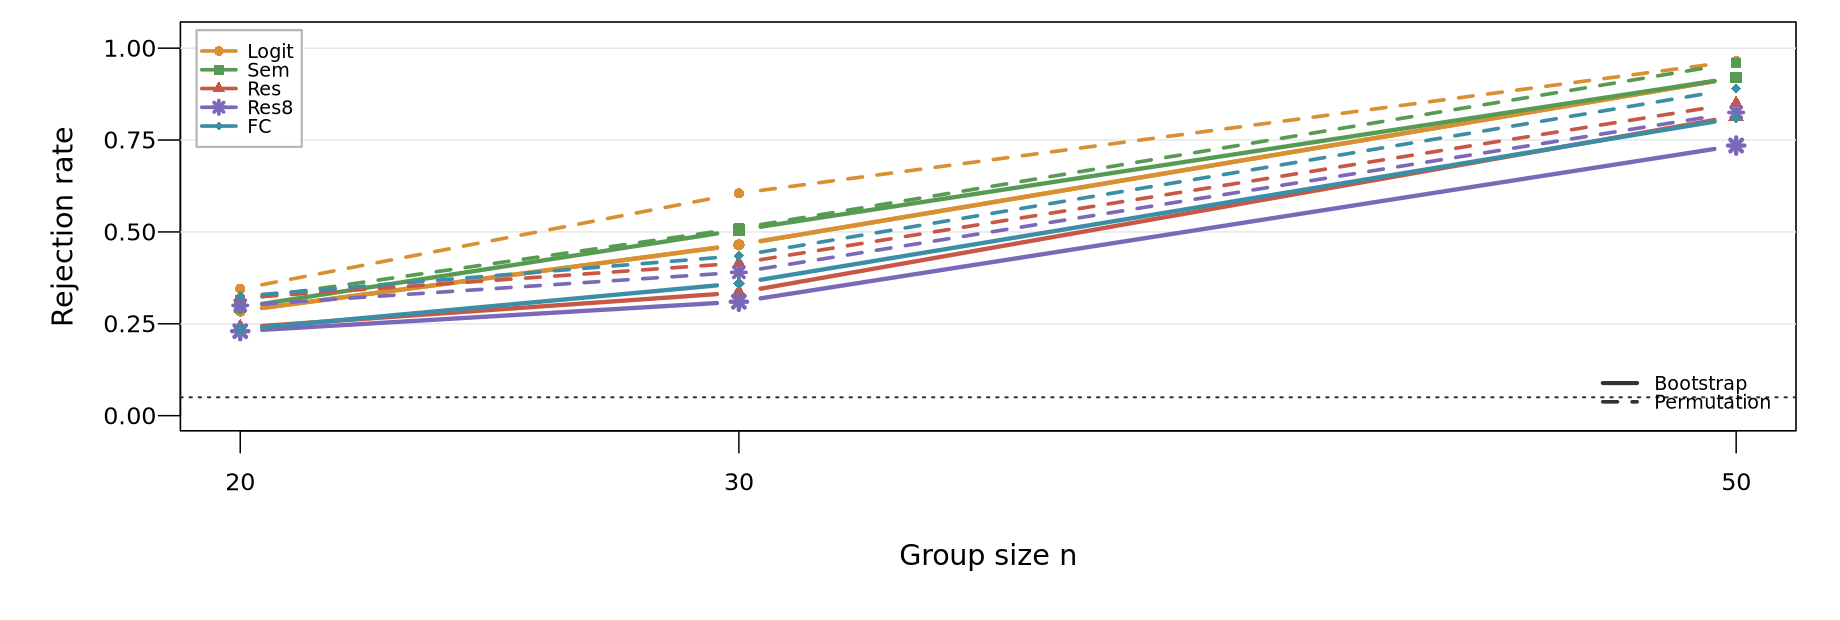
\includegraphics[width=\linewidth]{figures/dechao_permutation_bootstrap_label6.png}\\[-2pt]
\textbf{(a)} Label 6
\end{minipage}\hfill
\begin{minipage}[t]{0.49\textwidth}
\centering
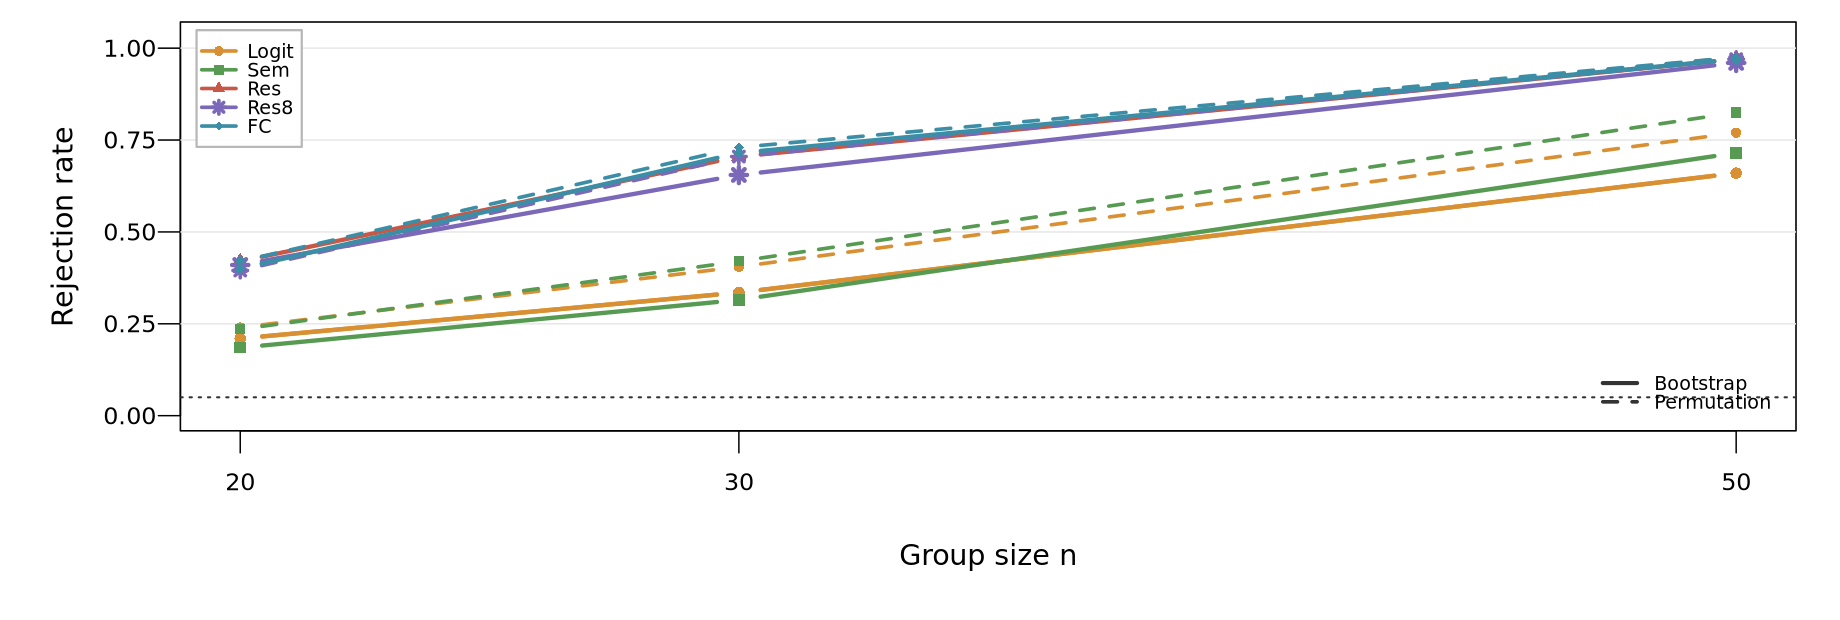
\includegraphics[width=\linewidth]{figures/dechao_permutation_bootstrap_label8.png}\\[-2pt]
\textbf{(b)} Label 8
\end{minipage}
\caption{Sensitivity comparison between multiplier-bootstrap and permutation calibration.}
\label{fig:app-dechao-permutation-check}
\end{figure}

\subsection{Two-stage explanation of the residual domain score}
\label{app:dechao-color-score-method}

This analysis used a train/holdout split and two fitted models. It was performed separately for the full residual feature and the top-eight residual PCA feature.

\paragraph{Stage 1: residual features to a domain score.}
On the training split, a logistic regression classified source ($D_i=0$) versus external ($D_i=1$) from residual feature $r_i$:
\[
\Pr(D_i=1\mid r_i)=\operatorname{logit}^{-1}(\beta_0+\beta^\top r_i).
\]
The continuous pre-sigmoid decision value
\[
s_i=\beta_0+\beta^\top r_i
\]
was called the residual source--external score. The fitted logistic model was then applied unchanged to holdout residual features to obtain out-of-sample scores. This score is not a tissue-class logit and is not treated as a biological outcome; it is a one-dimensional summary of the domain-separating direction learned from residual features.

\paragraph{Stage 2: color summaries to the residual score.}
For each image, a 15-dimensional color vector $c_i$ was extracted. For each of the red, green, and blue channels, the features were the pixel mean, pixel standard deviation, and the 10th, 50th, and 90th percentiles. Thus
\[
c_i=(\mu_R,\mu_G,\mu_B,\sigma_R,\sigma_G,\sigma_B,
q_{R,.1},q_{R,.5},q_{R,.9},q_{G,.1},q_{G,.5},q_{G,.9},q_{B,.1},q_{B,.5},q_{B,.9}).
\]
A linear regression was fitted on the training split,
\[
s_i=\alpha_0+\alpha^\top c_i+\varepsilon_i,
\]
and then applied unchanged to holdout color features. Holdout $R^2$ measured how much out-of-sample variation in the residual domain score could be predicted from color summaries.

\begin{figure}[H]
\centering
\begin{minipage}[t]{0.49\textwidth}
\centering
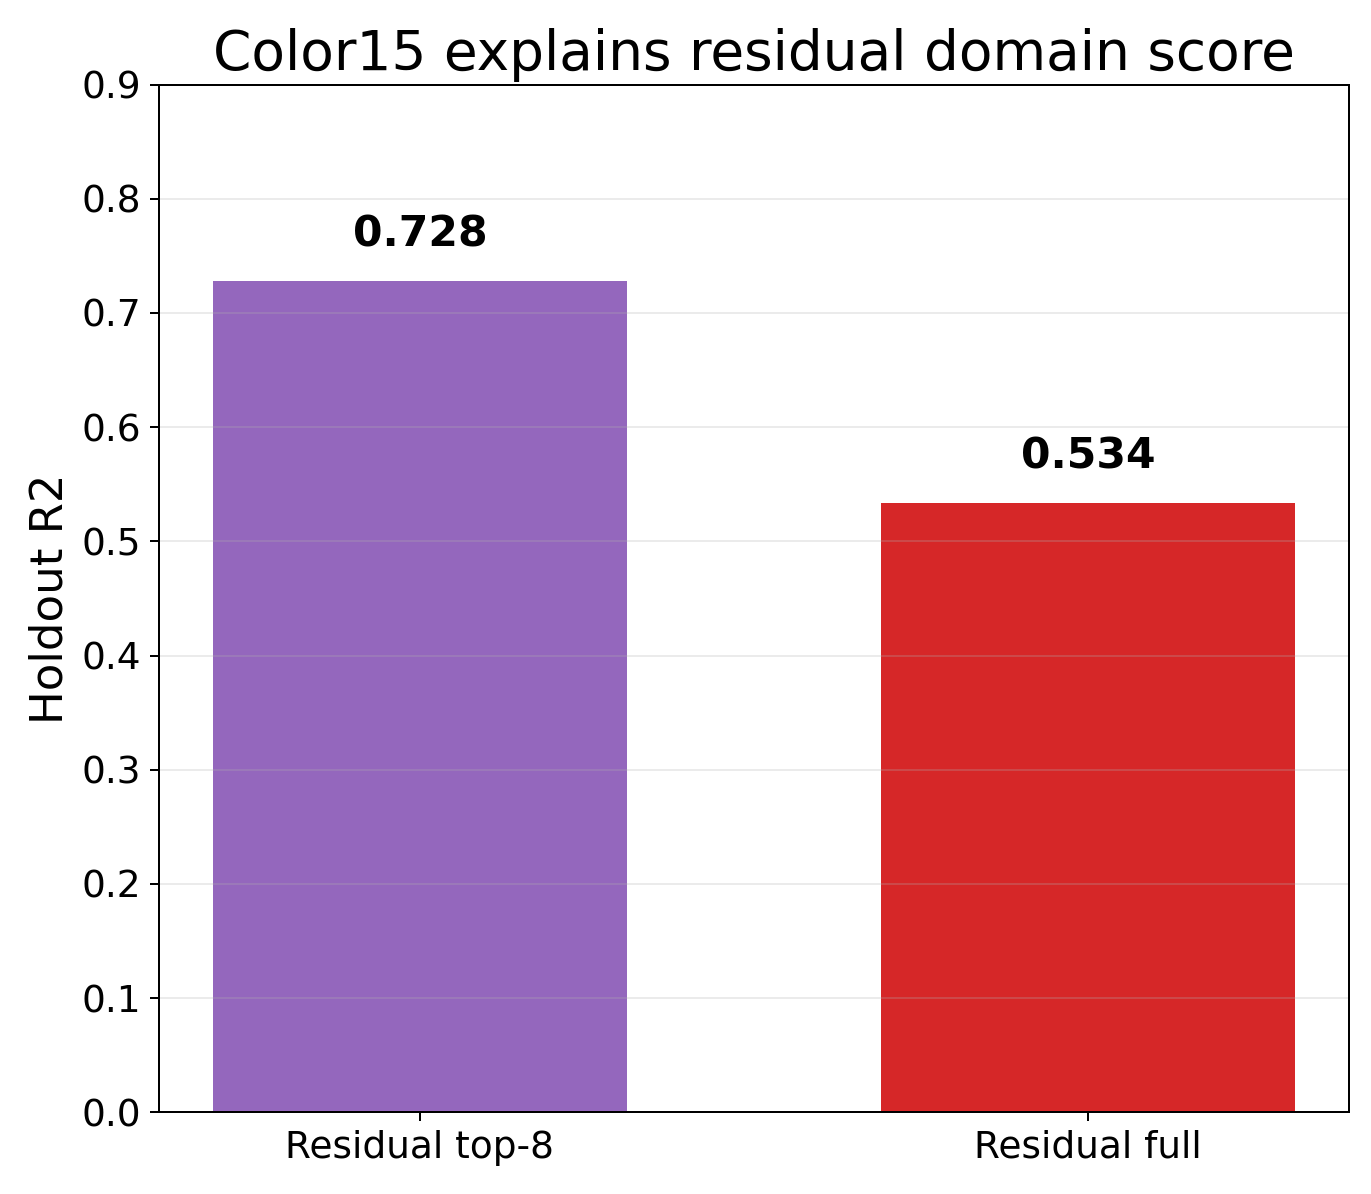
\includegraphics[width=\linewidth]{figures/dechao_color_score_r2.png}\\[-2pt]
\textbf{(a)} Holdout $R^2$ for the residual score
\end{minipage}\hfill
\begin{minipage}[t]{0.49\textwidth}
\centering
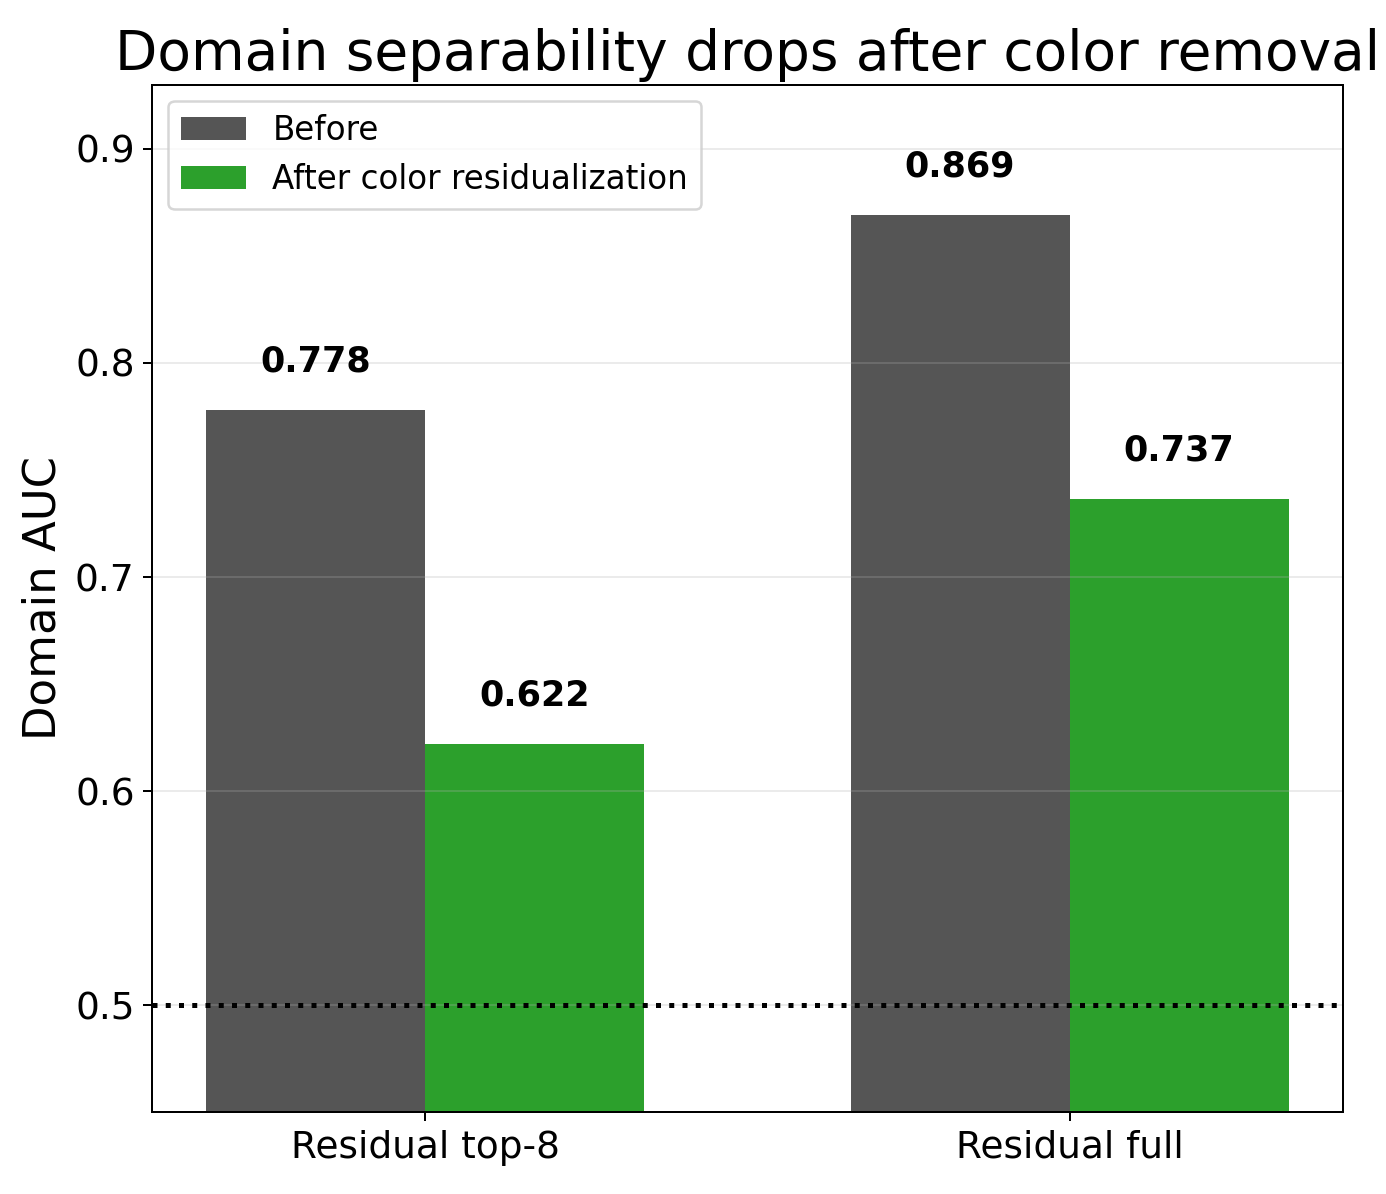
\includegraphics[width=\linewidth]{figures/dechao_color_score_auc_drop.png}\\[-2pt]
\textbf{(b)} AUROC before and after color-score residualization
\end{minipage}
\caption{Two-stage color explanation. Color summaries predict a substantial fraction of the residual source--external score, and removing that predicted component reduces held-out domain separability.}
\label{fig:app-dechao-color-score}
\end{figure}


For score residualization, the holdout color prediction $\widehat s_{i,\mathrm{color}}$ was subtracted from the holdout residual score:
\[
s_{i,\mathrm{adj}}=s_i-\widehat s_{i,\mathrm{color}}.
\]
AUROC was calculated against the source/external labels using $s_i$ before adjustment and $s_{i,\mathrm{adj}}$ after adjustment. AUC depends on the ranking of scores, not their absolute magnitude; subtracting a common constant would leave AUC unchanged. The observed AUC reduction therefore reflects removal of a sample-specific color-associated component. Both the logistic and linear models were fitted only on the training split, and all reported $R^2$ and AUC values were computed on holdout images.

\subsection{Color-only MMMD and color-propensity matching}
\label{app:dechao-color-matching-method}

The color-only analysis used the 15-dimensional vectors $c_i$ directly as MMMD inputs. The alternative compared label-8 source and external color vectors; source-internal and external-internal tests provided null references. Thus this experiment asked whether simple RGB summaries alone were sufficient to detect the domain difference.

For matching, a separate logistic propensity model was fitted using color summaries:
\[
p_i=\Pr(D_i=1\mid c_i),\qquad \eta_i=\log\frac{p_i}{1-p_i}.
\]
Source and external images were paired by nearest propensity logit $\eta_i$ under the implementation's caliper. The procedure retained 846 source--external pairs, with mean absolute within-pair logit gap 0.009. Pairing was used only to select color-balanced cohorts: after matching, all selected source observations were pooled into one group and all selected external observations into the other, and residual MMMD was applied to these two groups. It was not a paired-sample MMMD statistic.

The matched alternative sampled one group from the matched source cohort and one from the matched external cohort. Matched $H_0$-source and $H_0$-external were formed by drawing both groups from the same matched cohort. The displayed ``max matched $H_0$'' is the larger of these two internal-null rejection rates. Matching targets between-group color balance; it does not force either matched cohort to become internally homogeneous. The matched color-only AUC was 0.632, so residual color imbalance remained and the matched analysis should not be interpreted as perfect color randomization.

\begin{figure}[H]
\centering
\begin{minipage}[t]{0.49\textwidth}
\centering
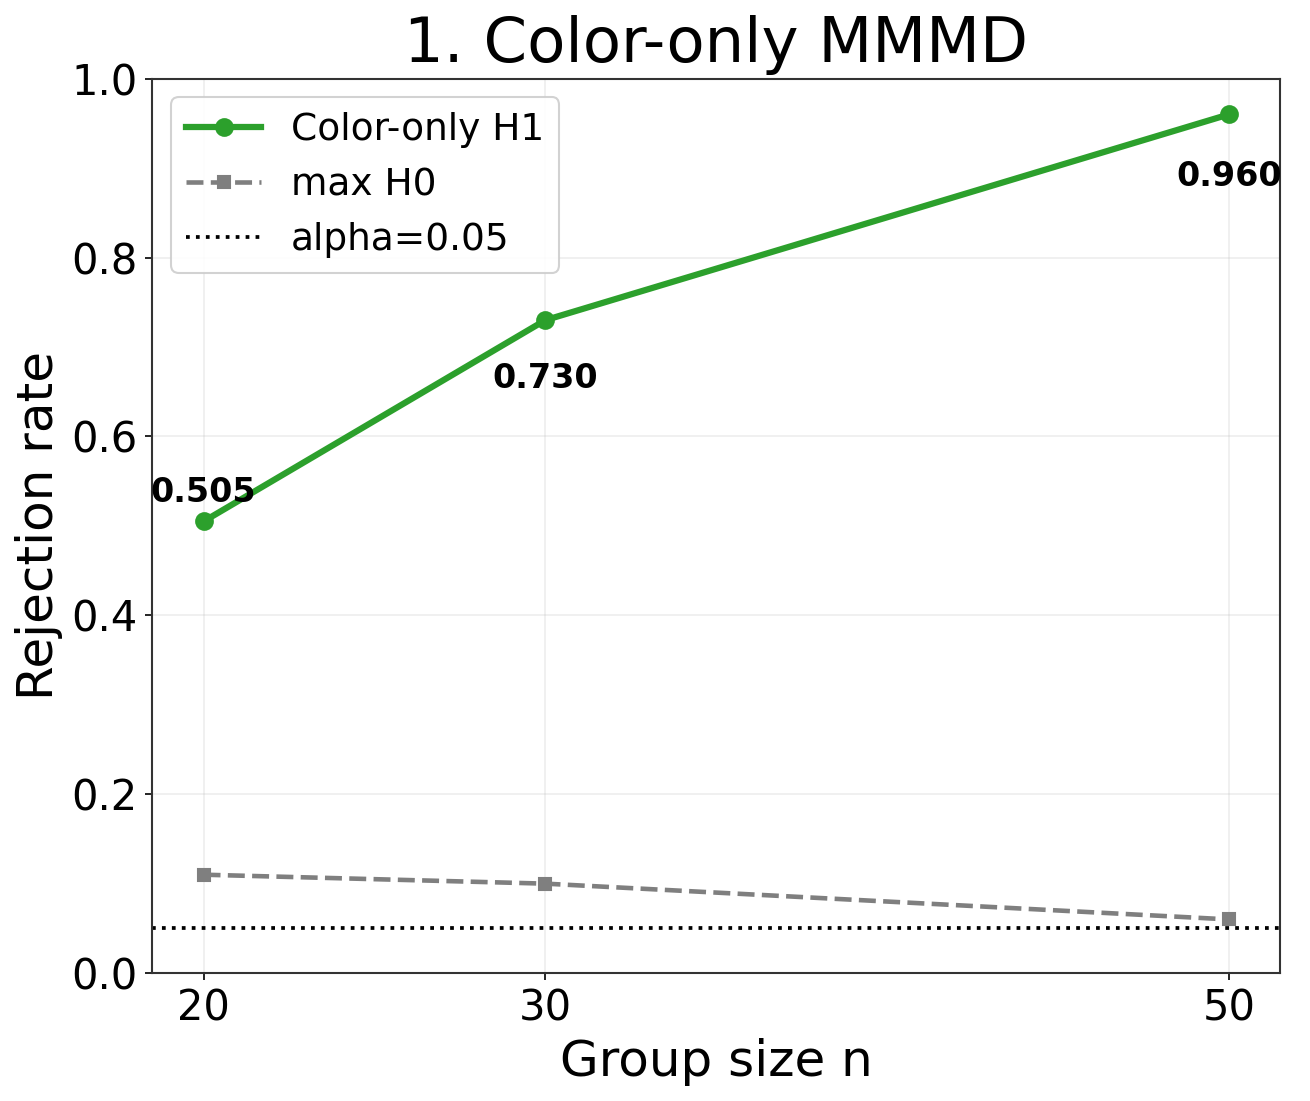
\includegraphics[width=\linewidth]{figures/dechao_color_only_mmmd.png}\\[-2pt]
\textbf{(a)} MMMD using only the 15 color summaries
\end{minipage}\hfill
\begin{minipage}[t]{0.49\textwidth}
\centering
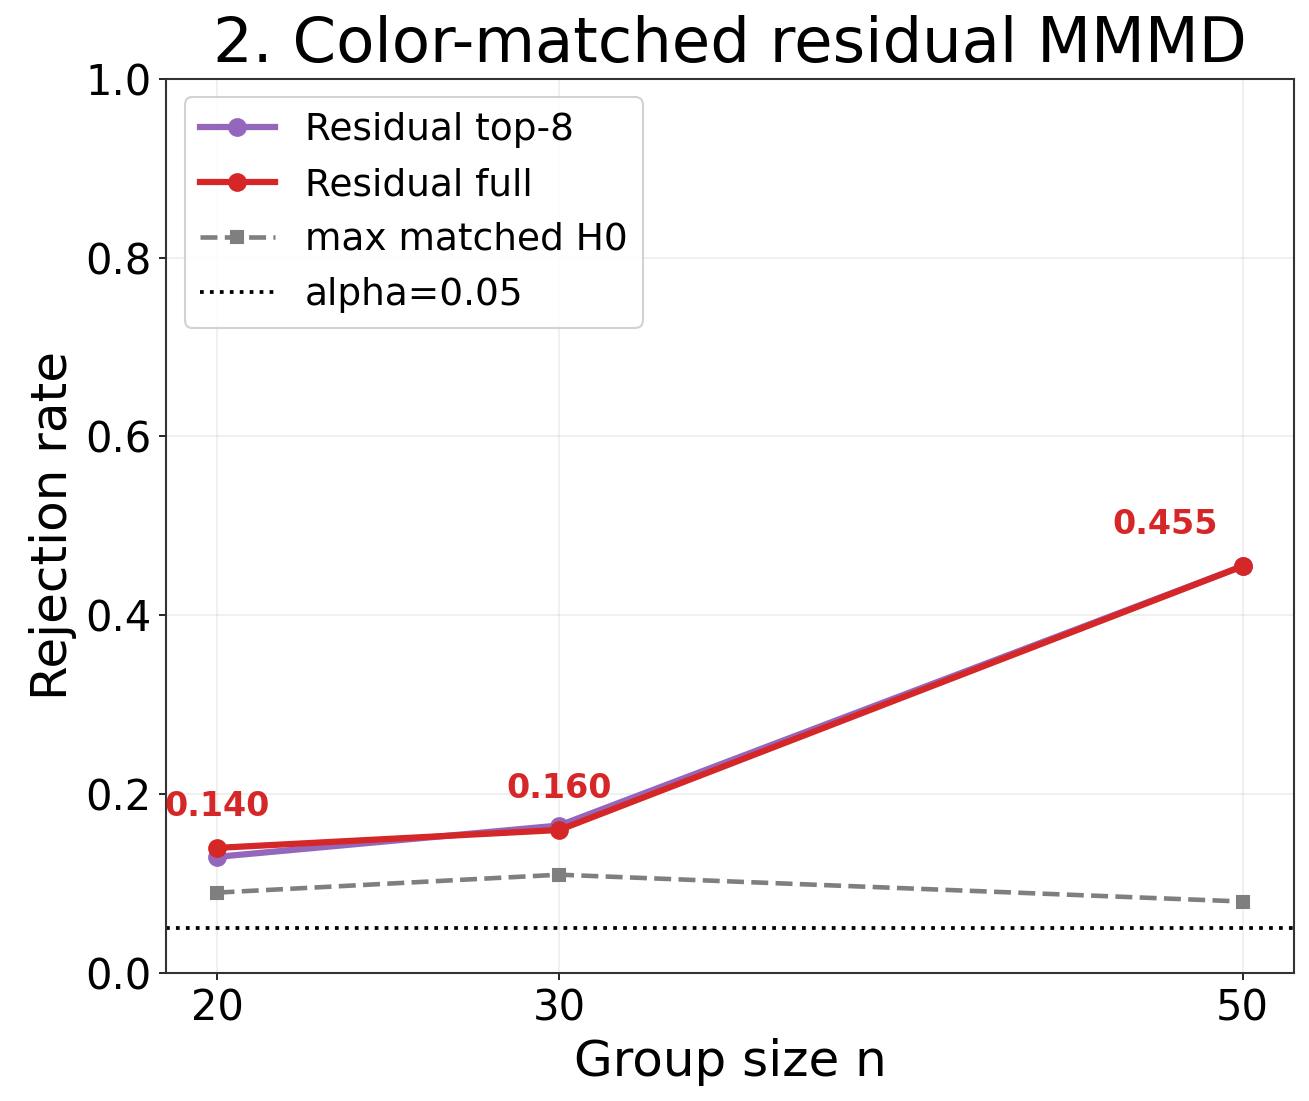
\includegraphics[width=\linewidth]{figures/dechao_color_matched_summary_residual.png}\\[-2pt]
\textbf{(b)} Residual MMMD after color-propensity matching
\end{minipage}
\caption{Direct color controls for label 8. Color summaries alone distinguish source and external images; after color matching, residual rejection is substantially reduced and is compared with the matched internal-null reference.}
\label{fig:app-dechao-color-mmmd}
\end{figure}

\subsection{Scope of the image-level inference}

All PathMNIST analyses are patch-level comparisons. Patient, slide, and scanner identifiers were not available in the packaged data used here, so the repeated-sampling calculations treat image patches as the observational units. Center-shift rejection therefore establishes a difference between the source and external patch distributions; it does not by itself identify a causal center effect or a patient-level biological difference. Likewise, color-score regression and propensity matching are diagnostic adjustments for measured RGB summaries, not a complete stain-normalization or causal mediation analysis.

\clearpage
\section{Detailed representation experiment tables and figures}
\label{app:repr}

\subsection{Datasets, tasks, and implementation details}

The representation experiments use three biomedical image datasets. BloodMNIST-224 contains 17,092 blood-cell images and is used for noise robustness and sample-size studies. PathMNIST-28 contains 107,180 small pathology patches and is used to compare frozen encoders with task-trained CNN baselines from the reproduction pipeline. NCT-CRC contains 100,000 H\&E patches and is used for larger pathology-image sample-size experiments and for the NEW-MMMD testing-layer comparison.

The BloodMNIST mixed alternative compares class-balanced mixtures \((0,1,3)\) and \((0,1,6)\), so the two populations share labels 0 and 1 and differ through labels 3 versus 6. The PathMNIST experiment follows the reproduction-aligned overlapping-mixture setting. The NCT-CRC alternative compares \((\mathrm{NORM}, \mathrm{STR}, \mathrm{LYM})\) with \((\mathrm{TUM}, \mathrm{STR}, \mathrm{LYM})\). These settings are harder than direct binary class tests because only part of the mixture changes.

CLIP and DINOv2 are used as frozen foundation encoders. CLIP is trained by aligning images with natural-language text, so its representation tends to emphasize semantic concepts that are useful for image--text matching. DINOv2 is trained by self-supervised visual learning and is often more sensitive to visual texture, local structure, and morphology. This distinction motivates comparing both encoders rather than treating foundation features as a single category.

The implementation used for this section is organized under \path{code/Biostatistics_fdu_26/yao}. The shared R testing functions are in \path{code/Biostatistics_fdu_26/yao/src/mmmd_functions.R}, and the slide-based experiment narrative is stored under \path{representation_final_package}. Most representation comparisons use GAUSS5; the NEW-MMMD experiment is the main exception because it explicitly changes the testing layer.

\begin{figure}[H]
\centering
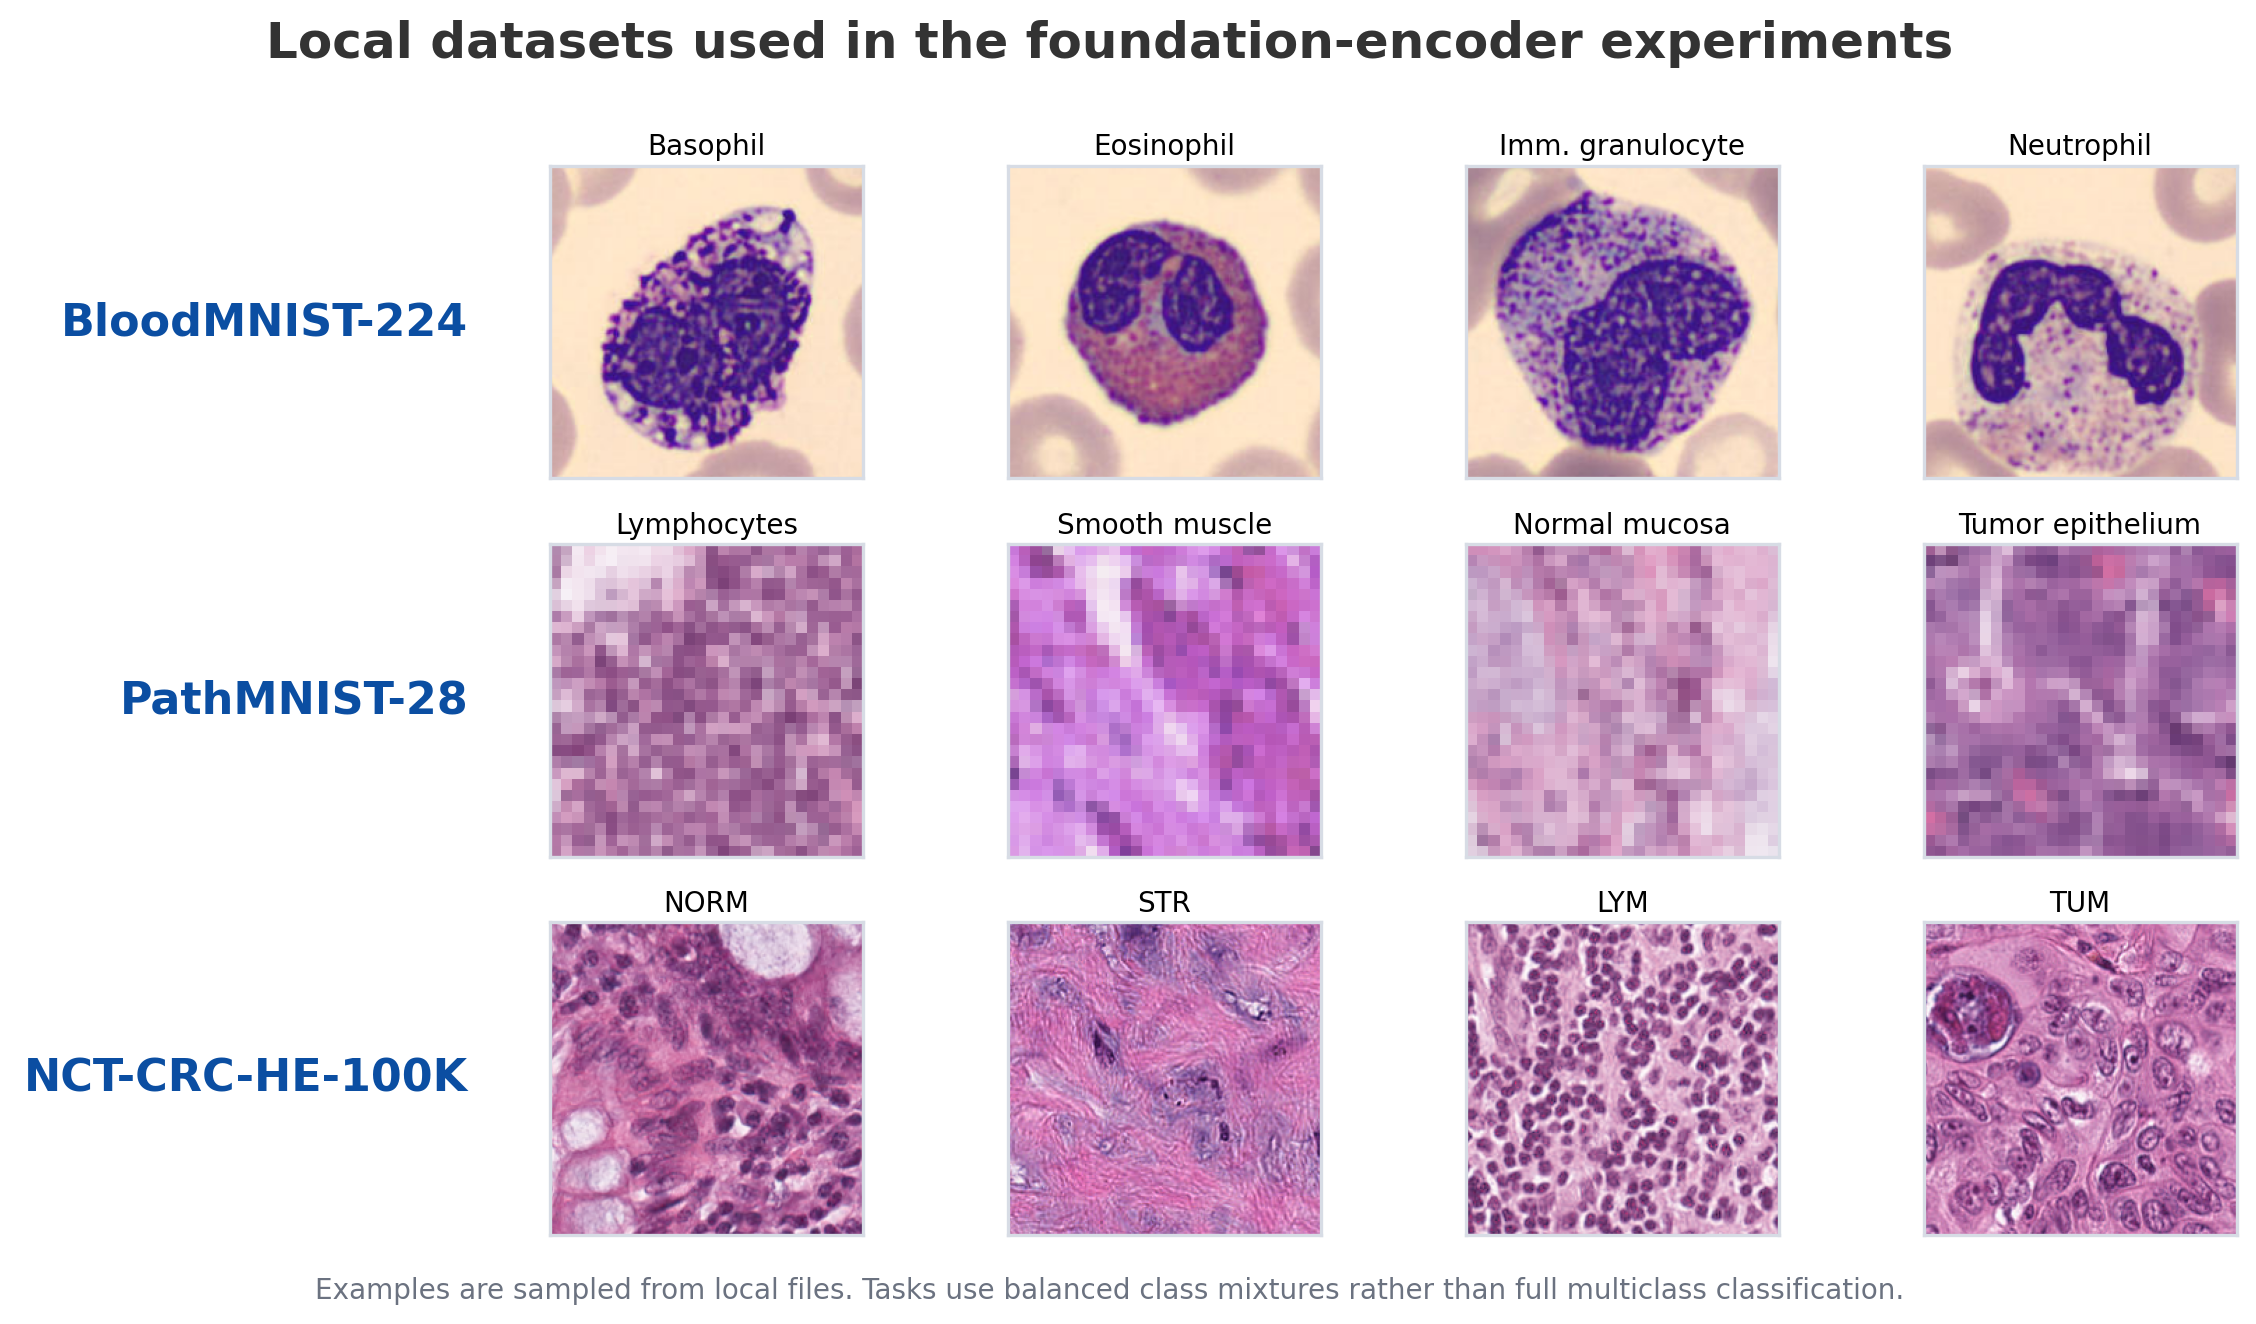
\includegraphics[width=0.88\textwidth]{figures/foundation_dataset_examples.png}
\caption{Biomedical image datasets used in the representation experiments.}
\label{fig:dataset-examples}
\end{figure}

\begin{figure}[H]
\centering
\begin{minipage}[t]{0.49\textwidth}
\centering
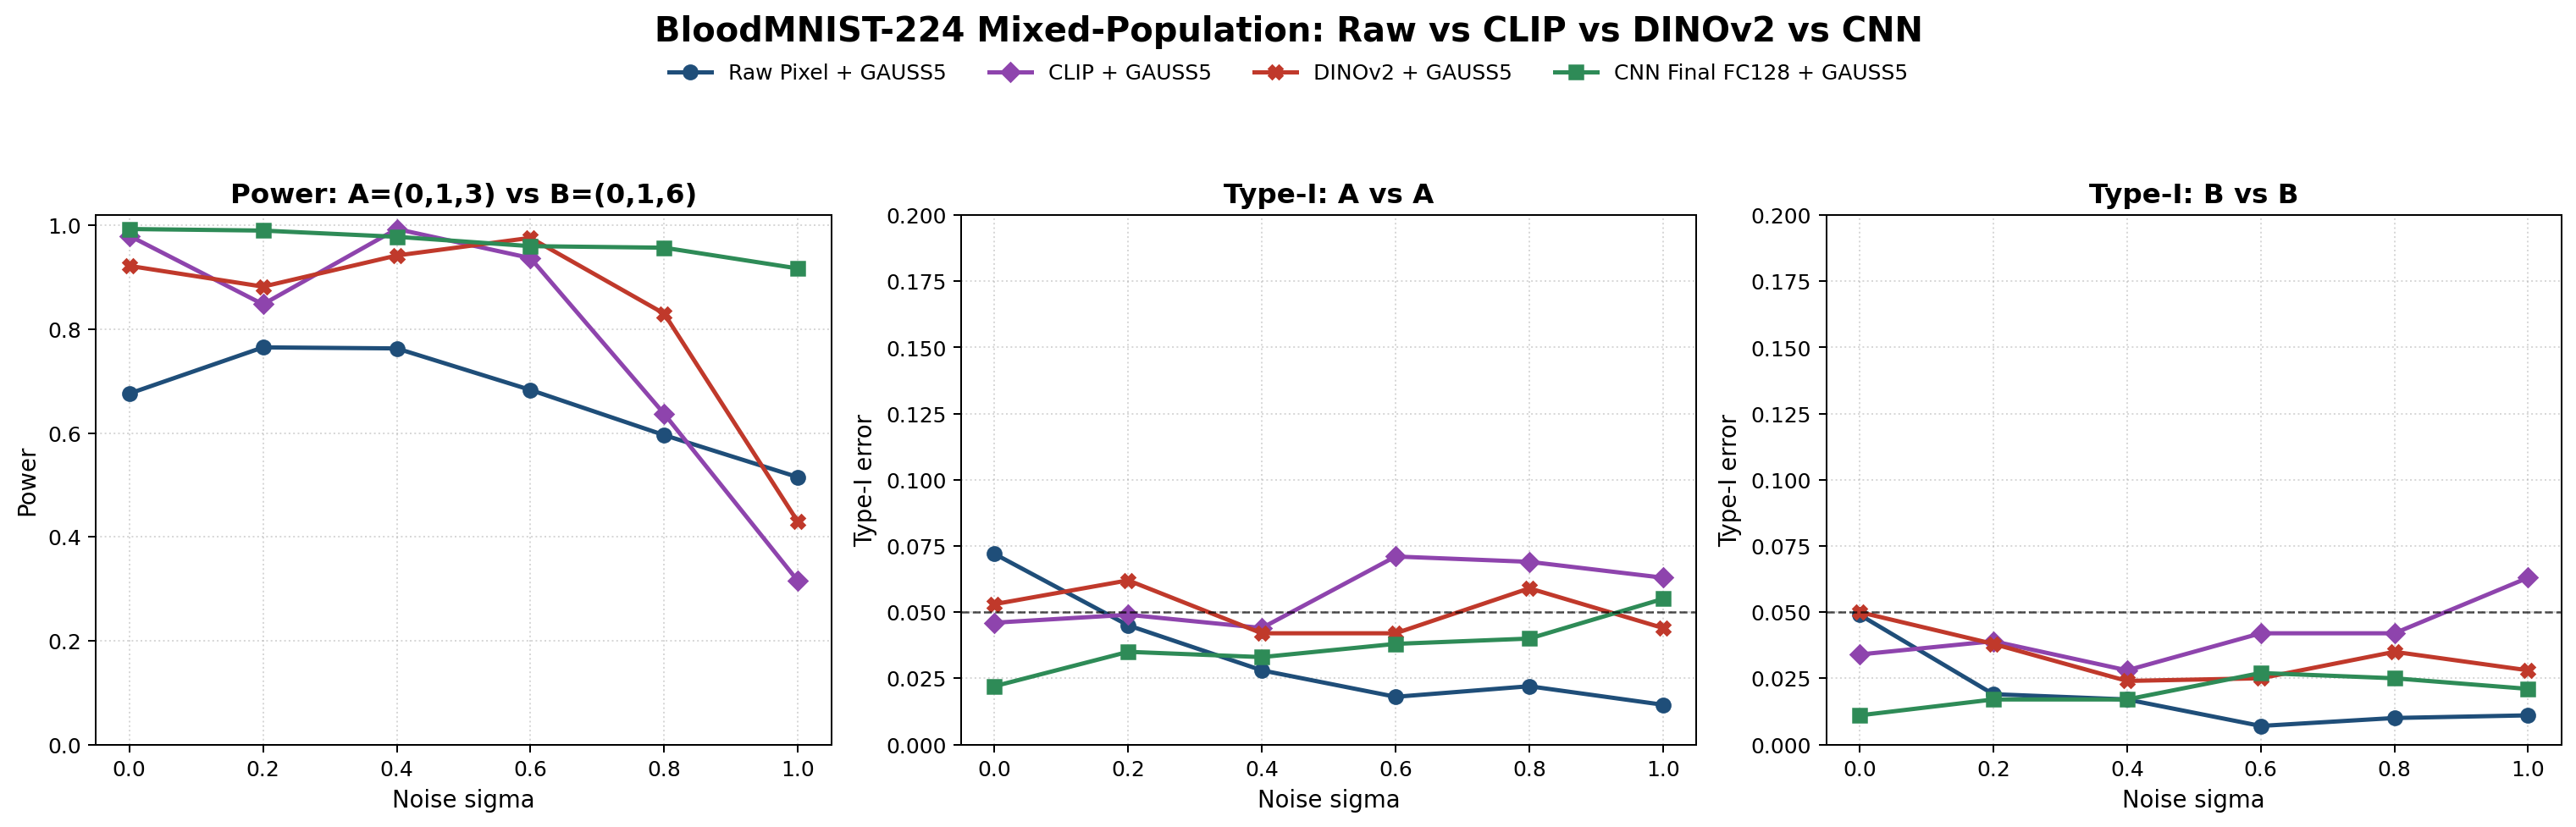
\includegraphics[width=\linewidth]{figures/bloodmnist_mixed_raw_clip_dino_cnn_gauss5.png}
\end{minipage}\hfill
\begin{minipage}[t]{0.49\textwidth}
\centering
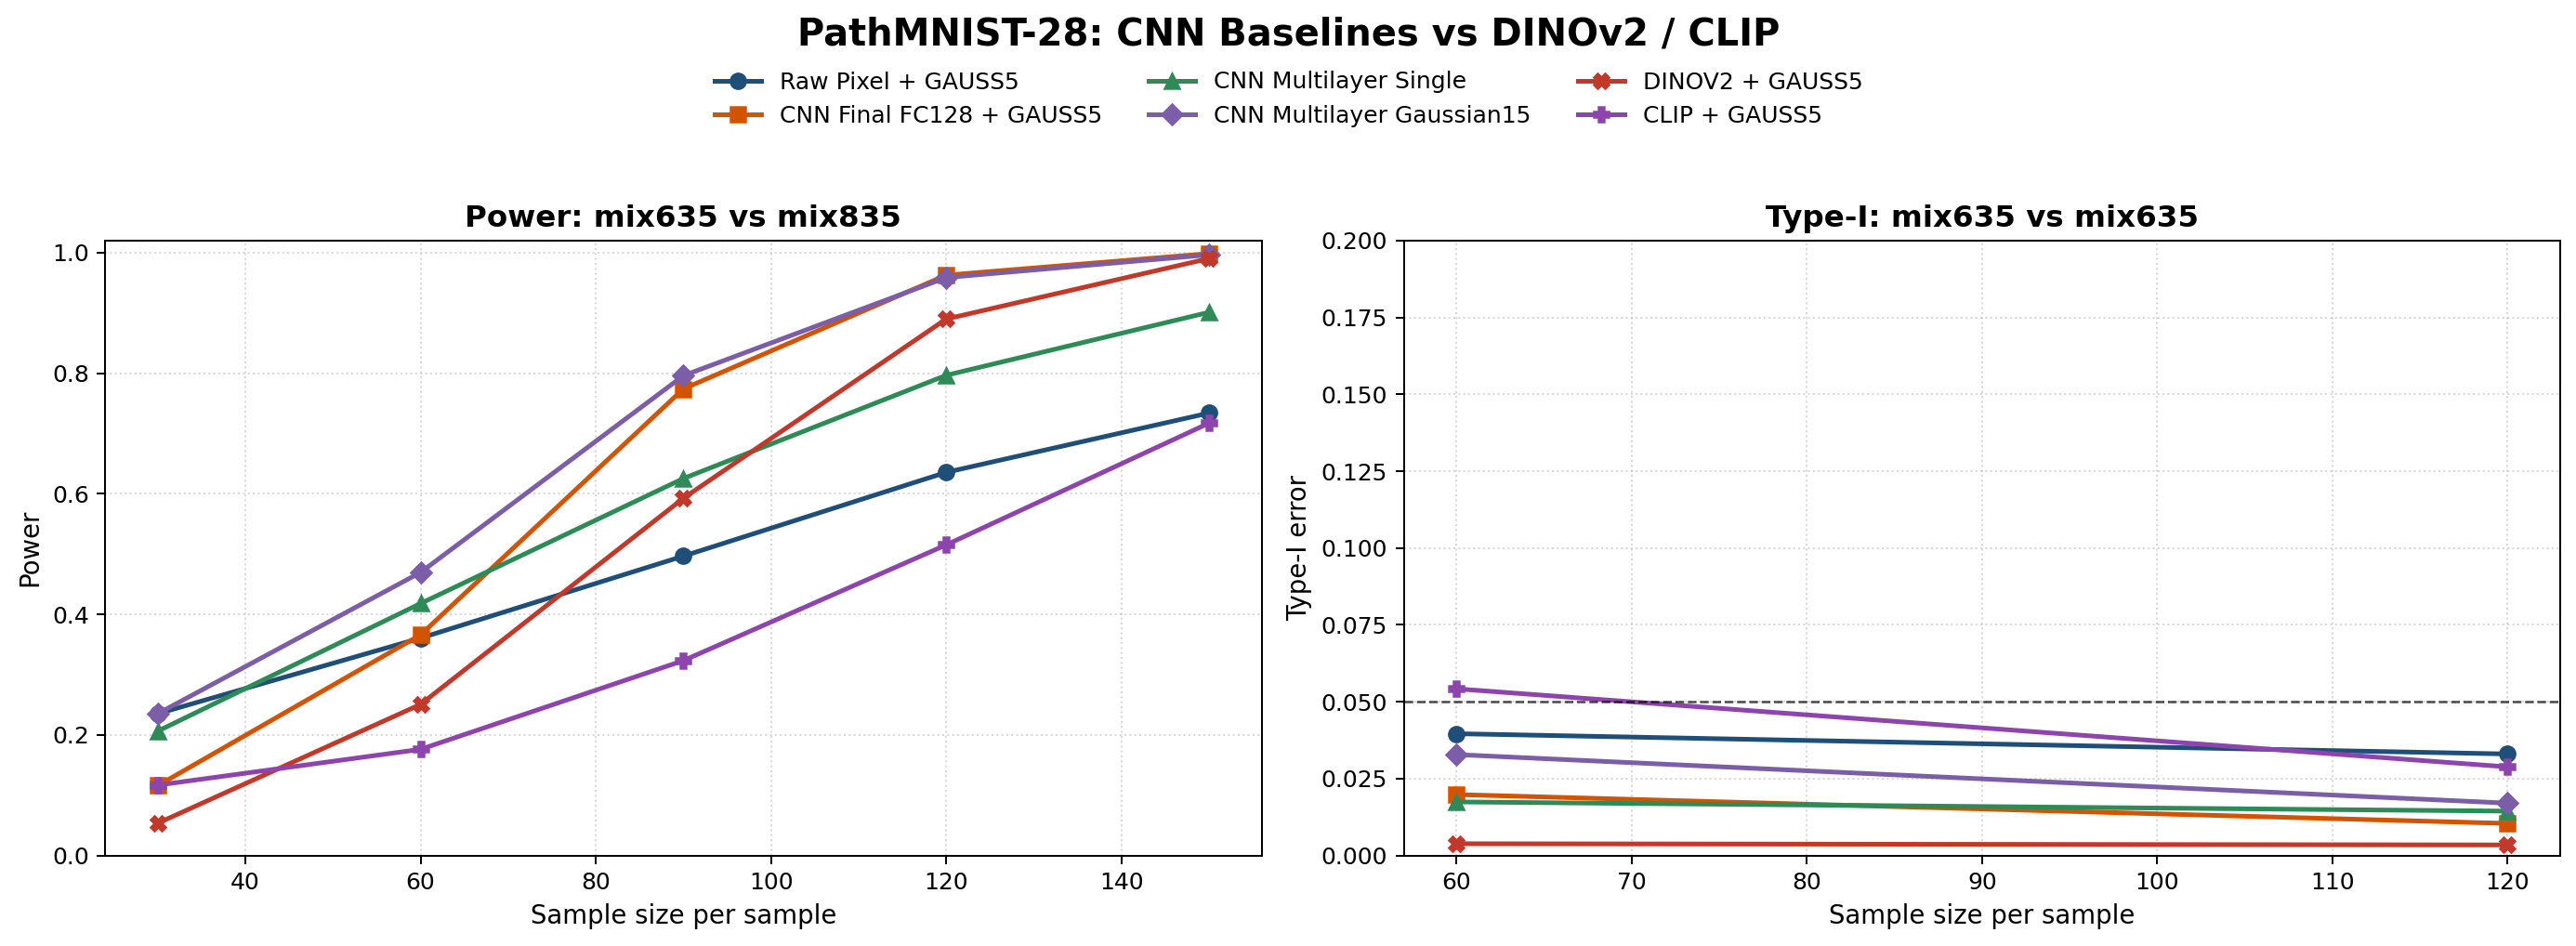
\includegraphics[width=\linewidth]{figures/pathmnist_sample_size_vs_cnn.png}
\end{minipage}
\caption{BloodMNIST and PathMNIST representation experiments.}
\label{fig:blood-path-app}
\end{figure}

\begin{table}[H]
\centering
\caption{BloodMNIST mixed task power at endpoint noise levels.}
\label{tab:blood-endpoints}
\begin{tabular}{lcc}
\toprule
Representation & Power at \(\sigma=0\) & Power at \(\sigma=1\) \\
\midrule
Raw pixels & 0.676 & 0.515 \\
CLIP & 0.980 & 0.315 \\
DINOv2 & 0.922 & 0.429 \\
CNN final FC-128 & 0.993 & 0.917 \\
\bottomrule
\end{tabular}
\end{table}

\begin{figure}[H]
\centering
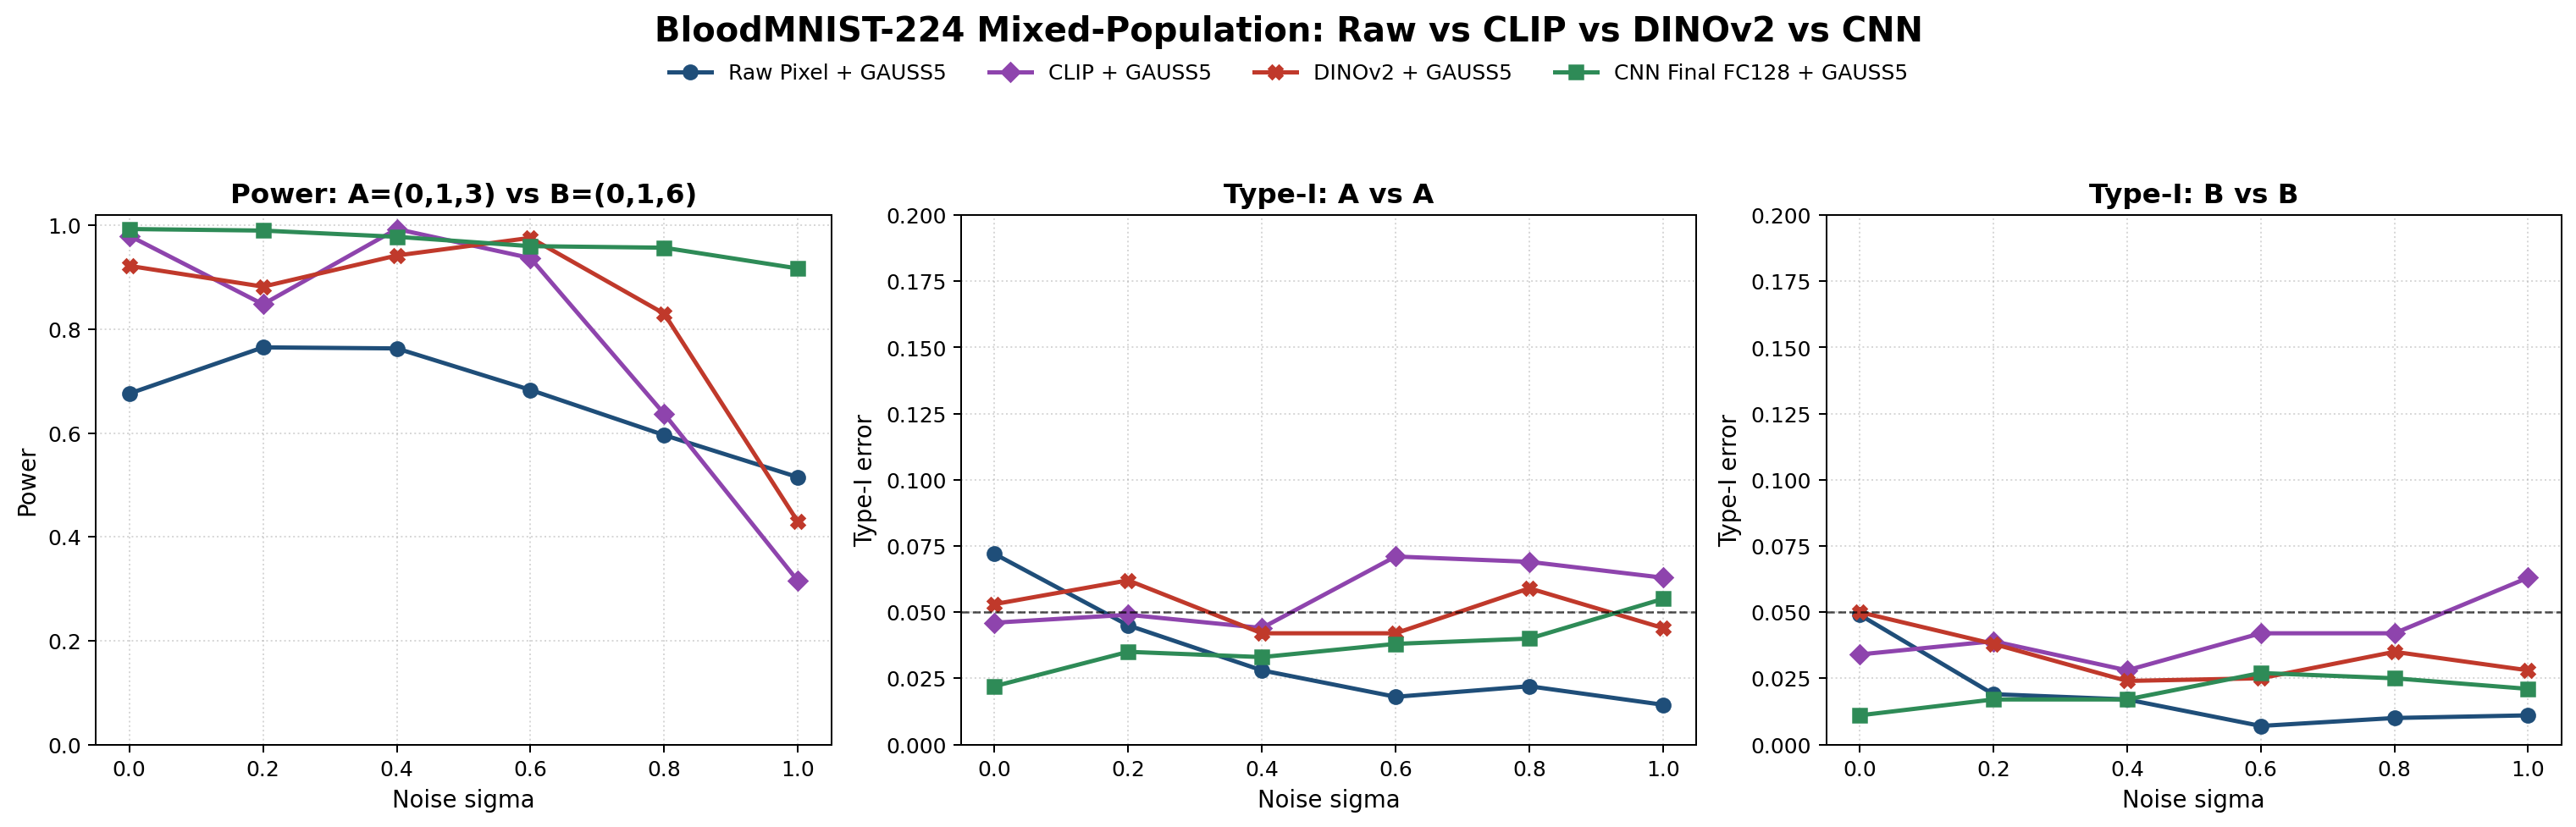
\includegraphics[width=0.74\textwidth]{figures/bloodmnist_mixed_raw_clip_dino_cnn_gauss5.png}
\caption{BloodMNIST mixed-task representation comparison.}
\label{fig:blood-repr}
\end{figure}

\begin{table}[H]
\centering
\caption{BloodMNIST sample-size sweep at fixed \(\sigma=0.6\).}
\label{tab:blood-sample-size}
\begin{tabular}{rrrr}
\toprule
Sample size & Raw pixels & CLIP & DINOv2 \\
\midrule
30 & 0.0625 & 0.5000 & 0.5125 \\
60 & 0.4125 & 0.7750 & 0.8875 \\
90 & 0.7125 & 0.8875 & 0.9625 \\
120 & 0.8875 & 0.9625 & 1.0000 \\
150 & 0.9875 & 1.0000 & 1.0000 \\
\bottomrule
\end{tabular}
\end{table}

\begin{figure}[H]
\centering
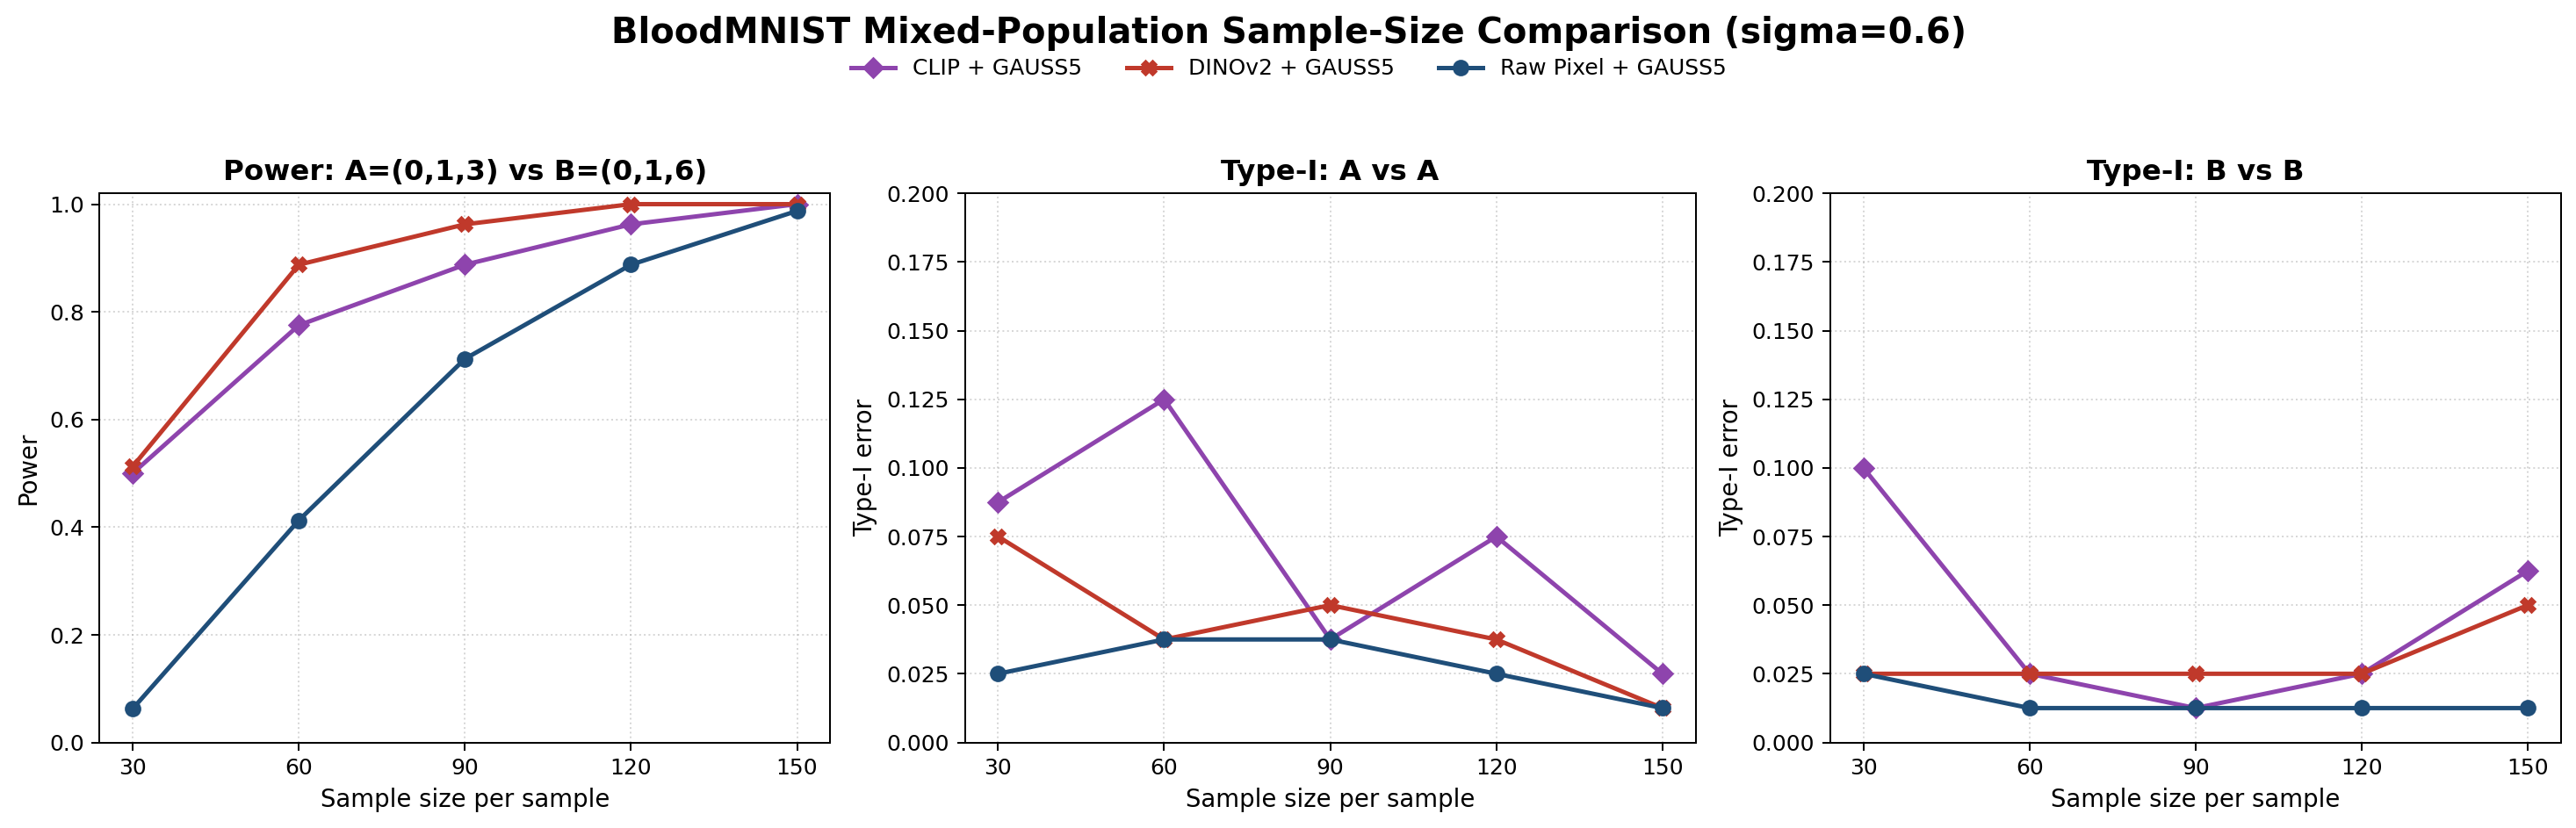
\includegraphics[width=0.74\textwidth]{figures/bloodmnist_mixed_sample_size_comparison.png}
\caption{BloodMNIST sample-size comparison at \(\sigma=0.6\).}
\label{fig:blood-sample}
\end{figure}

\begin{table}[H]
\centering
\caption{PathMNIST frozen-encoder power in the reproduction-aligned overlapping-mixture setting.}
\label{tab:pathmnist}
\begin{tabular}{rrr}
\toprule
Sample size & CLIP & DINOv2 \\
\midrule
30 & 0.1166 & 0.0534 \\
60 & 0.1760 & 0.2506 \\
90 & 0.3232 & 0.5926 \\
120 & 0.5152 & 0.8900 \\
150 & 0.7172 & 0.9904 \\
\bottomrule
\end{tabular}
\end{table}

\begin{figure}[H]
\centering
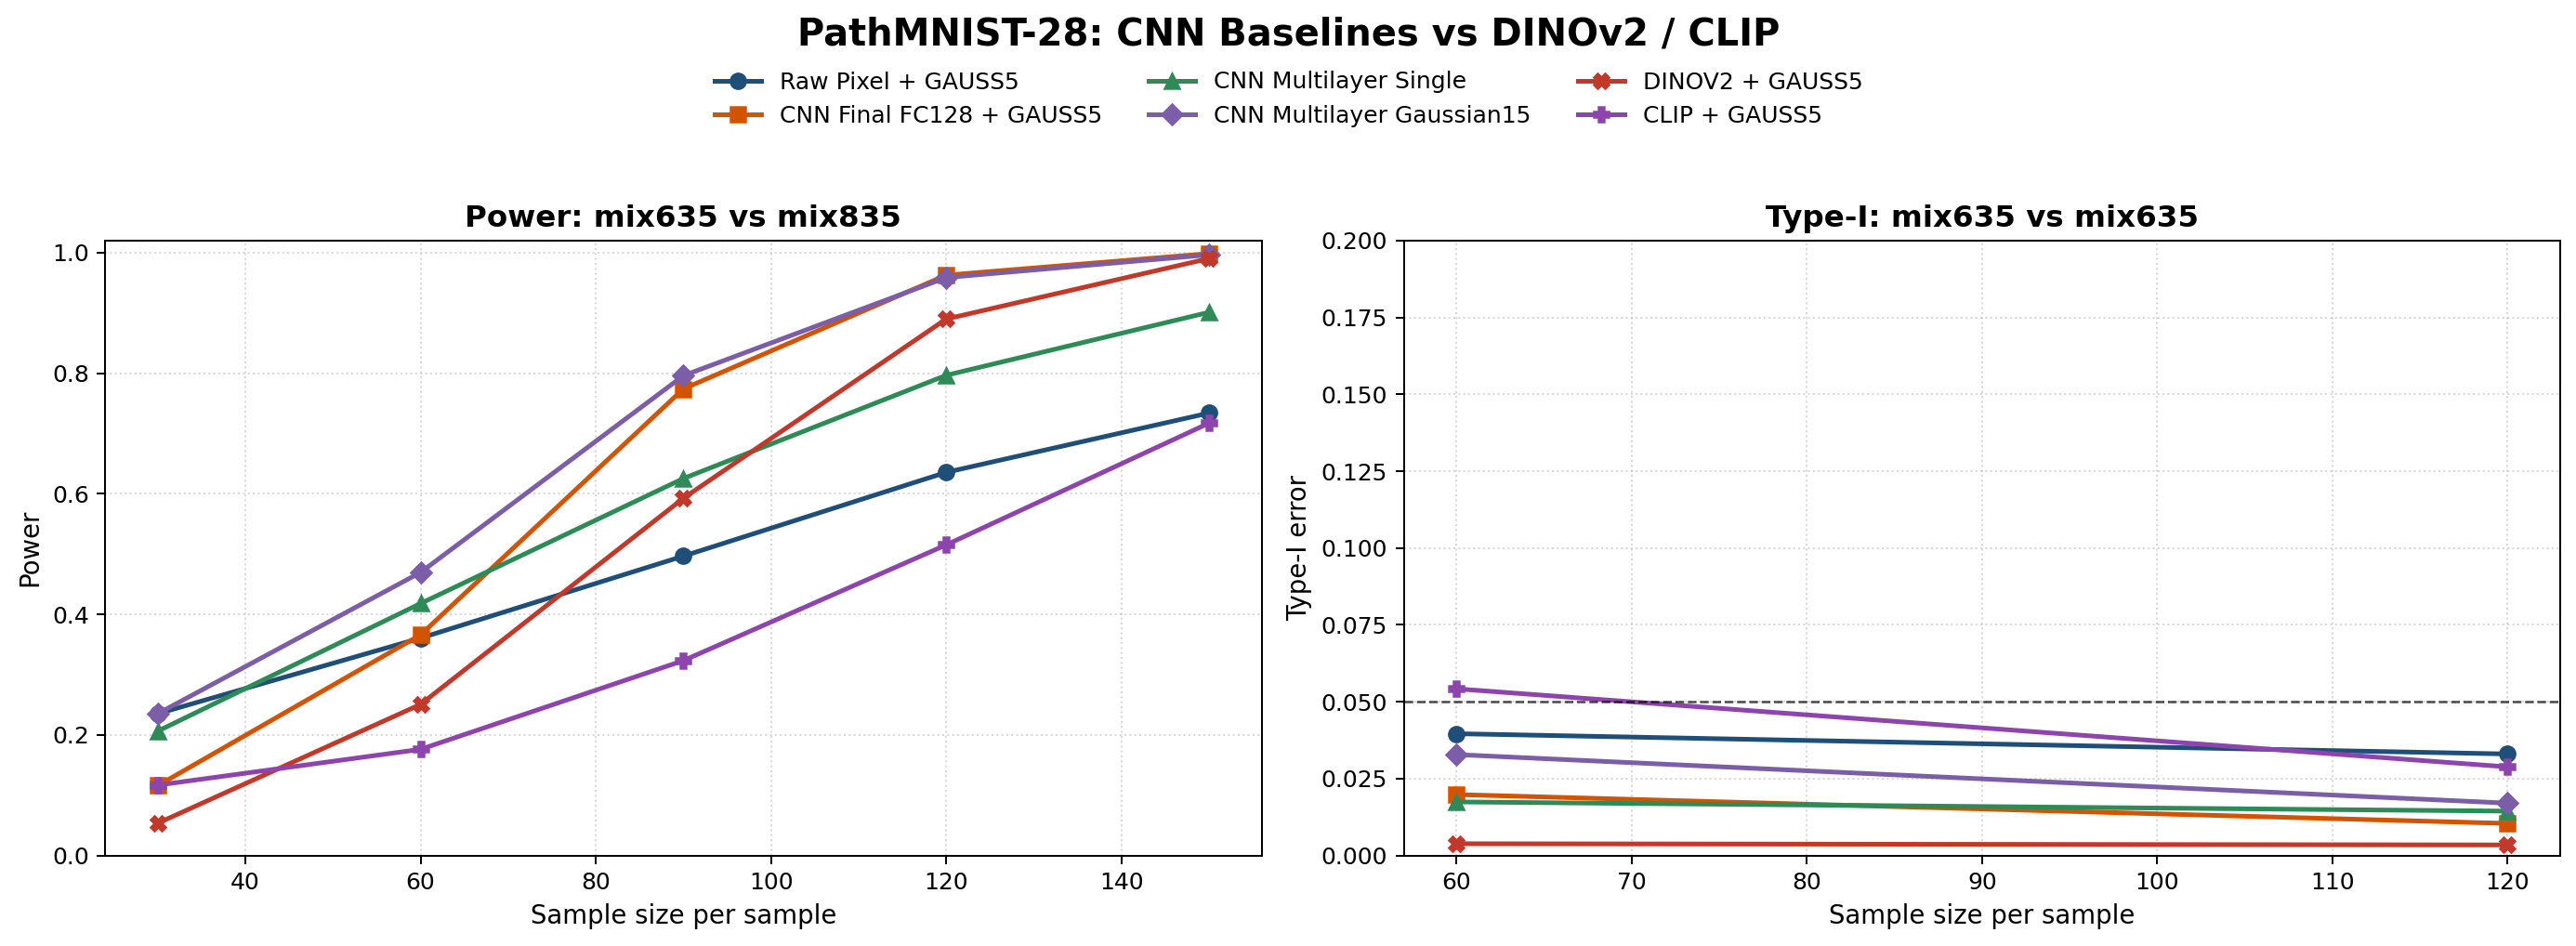
\includegraphics[width=0.74\textwidth]{figures/pathmnist_sample_size_vs_cnn.png}
\caption{PathMNIST frozen encoders compared with trained-CNN baselines.}
\label{fig:pathmnist}
\end{figure}

\begin{table}[H]
\centering
\caption{NCT-CRC representation comparison on \((\mathrm{NORM},\mathrm{STR},\mathrm{LYM})\) versus \((\mathrm{TUM},\mathrm{STR},\mathrm{LYM})\).}
\label{tab:nct}
\begin{tabular}{rrrrr}
\toprule
Sample size & Raw pixels & CLIP & CNN & DINOv2 \\
\midrule
30 & 0.125 & 0.013 & 0.100 & 0.038 \\
60 & 0.113 & 0.063 & 0.288 & 0.188 \\
90 & 0.175 & 0.200 & 0.575 & 0.475 \\
120 & 0.238 & 0.500 & 0.738 & 0.875 \\
150 & 0.300 & 0.750 & 0.875 & 0.988 \\
\bottomrule
\end{tabular}
\end{table}

\begin{figure}[H]
\centering
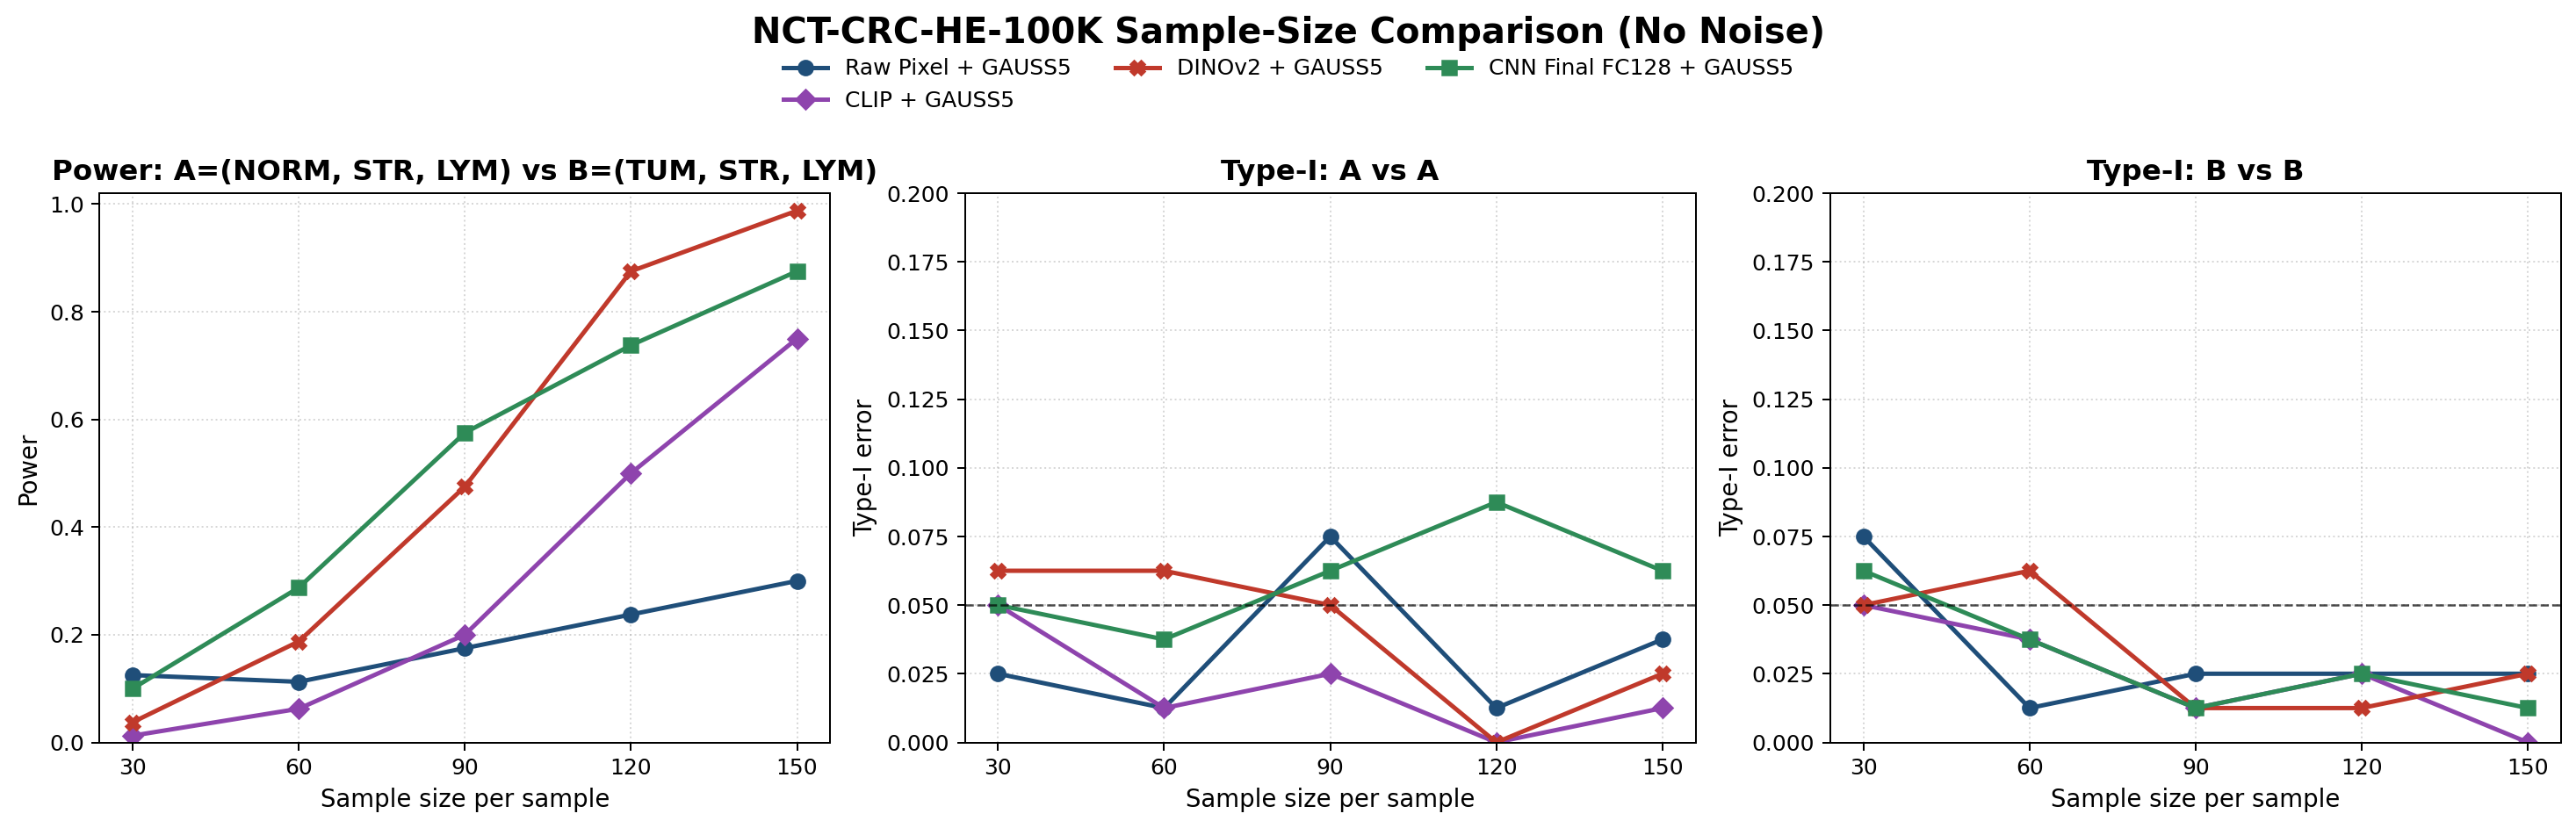
\includegraphics[width=0.74\textwidth]{figures/nctcrc_sample_size_comparison.png}
\caption{NCT-CRC representation comparison across sample sizes.}
\label{fig:nct}
\end{figure}

\begin{table}[H]
\centering
\caption{NCT-CRC DINOv2 testing-layer comparison.}
\label{tab:new-mmmd}
\begin{tabular}{rrr}
\toprule
Sample size & GEXP-5 power & NEW-MMMD power \\
\midrule
30 & 0.1000 & 0.0125 \\
60 & 0.1875 & 0.1500 \\
90 & 0.5625 & 0.5375 \\
120 & 0.9000 & 0.9125 \\
150 & 0.9625 & 0.9750 \\
\bottomrule
\end{tabular}
\end{table}

\begin{figure}[H]
\centering
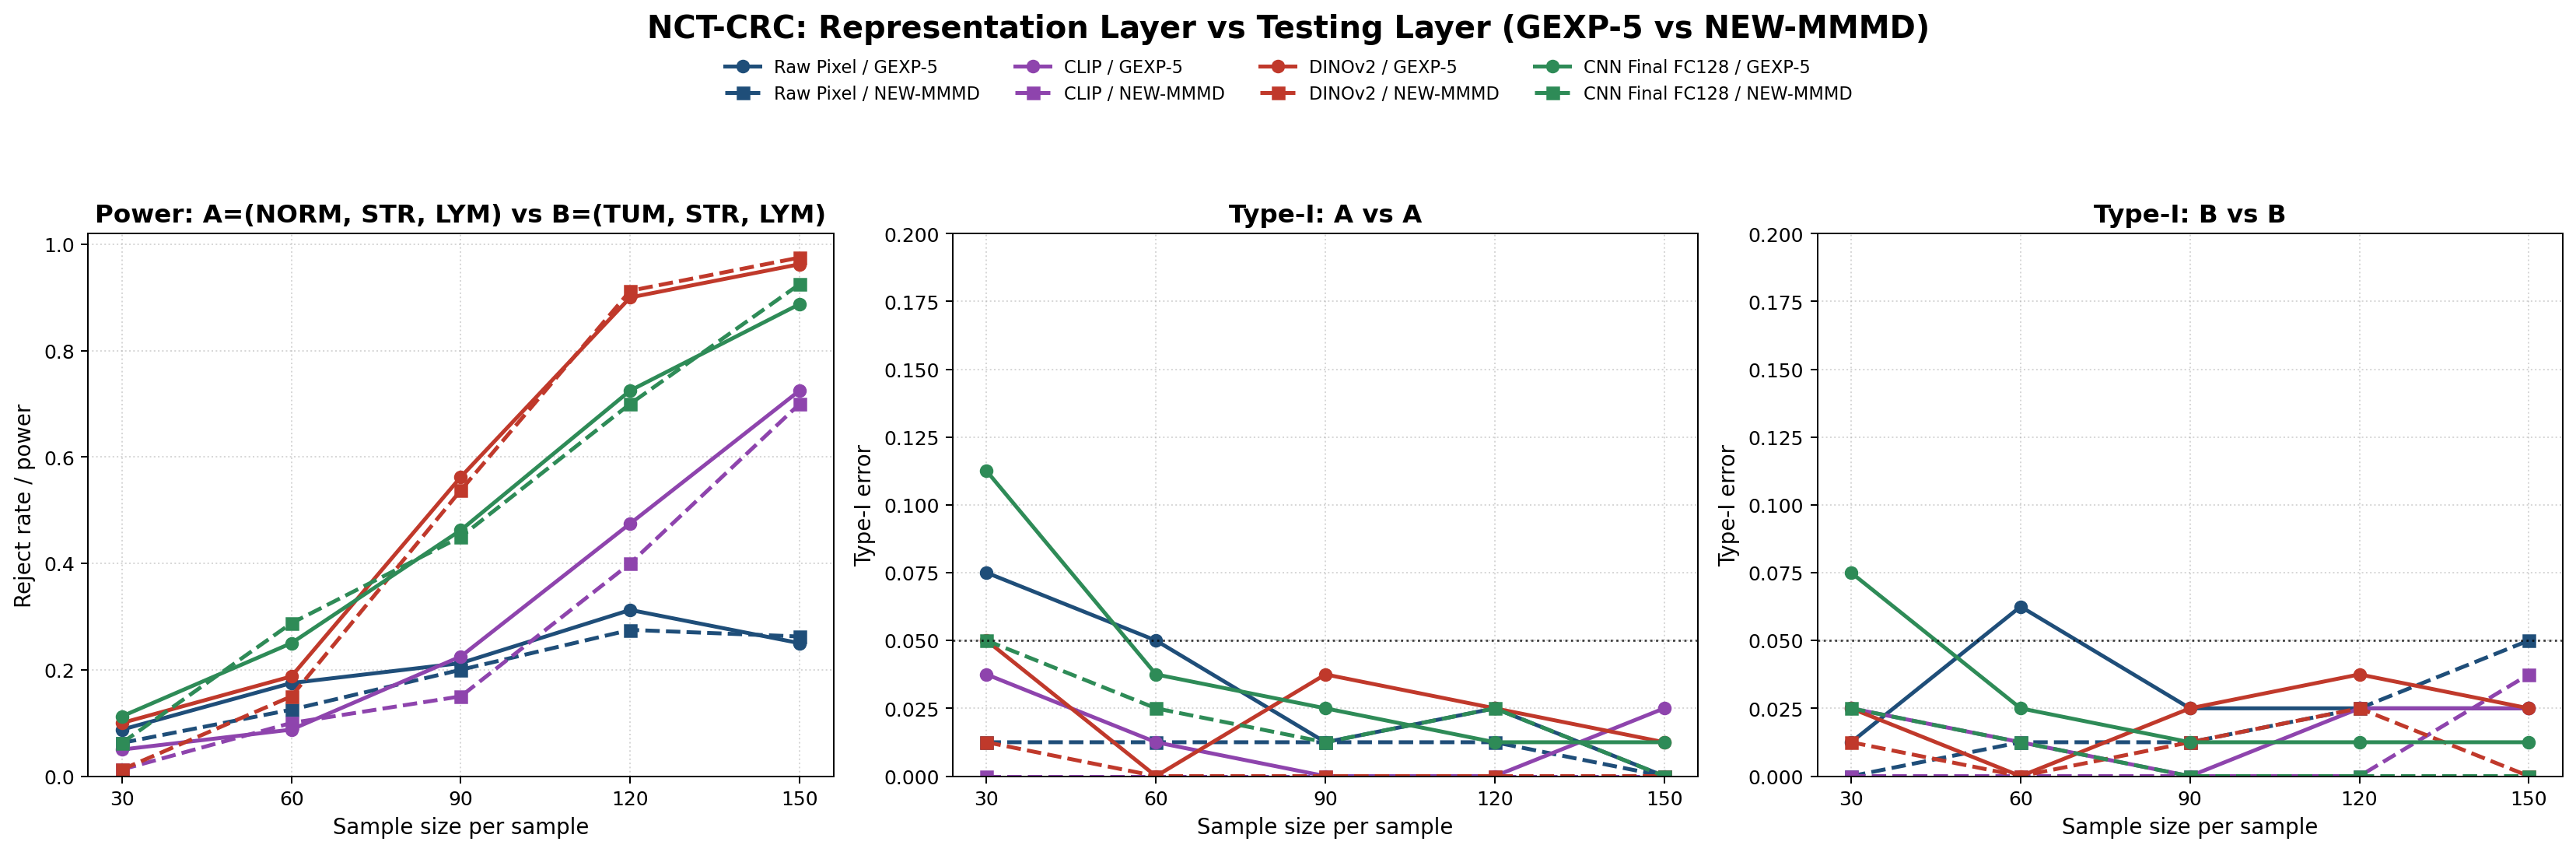
\includegraphics[width=0.74\textwidth]{figures/nctcrc_lrj_all_representations.png}
\caption{NEW-MMMD and GEXP-5 comparison across NCT-CRC representations.}
\label{fig:newmmmd}
\end{figure}

\begin{thebibliography}{9}

\bibitem{banerjee2019}
Banerjee, S., et al. (2019).
Adaptive multivariate two-sample testing for microbiome differential abundance.

\bibitem{chatterjee2025}
Chatterjee, D. and Bhattacharya, B. B. (2025).
Mahalanobis maximum mean discrepancy for boosting the power of kernel two-sample tests.

\bibitem{chernozhukov2013}
Chernozhukov, V., Chetverikov, D., and Kato, K. (2013).
Gaussian approximations and multiplier bootstrap for maxima of sums of high-dimensional random vectors.

\bibitem{friedman1979}
Friedman, J. H. and Rafsky, L. C. (1979).
Multivariate generalizations of the Wald-Wolfowitz and Smirnov two-sample tests.

\bibitem{gretton2012}
Gretton, A., Borgwardt, K. M., Rasch, M. J., Schoelkopf, B., and Smola, A. (2012).
A kernel two-sample test.

\bibitem{harbrecht2012}
Harbrecht, H., Peters, M., and Schneider, R. (2012).
On the low-rank approximation by the pivoted Cholesky decomposition.

\bibitem{liu2020}
Liu, F., Xu, W., Lu, J., Zhang, G., Gretton, A., and Sutherland, D. J. (2020).
Learning deep kernels for non-parametric two-sample tests.

\bibitem{ramdas2015}
Ramdas, A., Reddi, S. J., Poczos, B., Singh, A., and Wasserman, L. (2015).
On the decreasing power of kernel and distance based nonparametric hypothesis tests in high dimensions.

\bibitem{schrab2023}
Schrab, A., Kim, I., Albert, M., Laurent, B., Guedj, B., and Gretton, A. (2023).
MMD aggregated two-sample test.

\bibitem{sejdinovic2013}
Sejdinovic, D., Sriperumbudur, B., Gretton, A., and Fukumizu, K. (2013).
Equivalence of distance-based and RKHS-based statistics in hypothesis testing.

\end{thebibliography}

\end{document}
